%%%%%%%%%%%%%%%%%%%%%
%%%%% PREAMBULE %%%%%
%%%%%%%%%%%%%%%%%%%%%
\documentclass[a4paper,12pt,twoside]{book}
\usepackage{fontspec}

%%%%% Index %%%%%
\usepackage{index}
\usepackage{imakeidx}%pour les index, à charger avant hyperref
\makeindex
\makeindex[name=referentiels, title=Index des noms de référentiels]
\makeindex[name=ina, title=Index des termes concernant l'Institut national de l'Audiovisuel]

\usepackage[pdfusetitle, pdfsubject ={Mémoire TNAH}, pdfkeywords={institut national de l'audiovisuel; référentiel; thésaurus; vocabulaire contrôlé; vocabulaire hiérarchique; ontologie; web de données; Wikidata; liens; alignement}]{hyperref}
\usepackage[english, french]{babel}
\usepackage{morewrites}
\usepackage{tocbibind} %paquet pour mettre index et bib dans la toc

% configurer le document selon les normes de l'école
\usepackage[margin=2.5cm]{geometry}
\usepackage{setspace}
\onehalfspacing
\setlength\parindent{1cm}

\usepackage{lettrine}
\usepackage{minted}

%%%%% Dessin %%%%%
\usepackage{qtree}
\usepackage{pstricks}
\usepackage{tikz} %paquet pour dessiner ; à placer avant graphicx
\usepackage{graphicx} %paquet image
\usepackage{wrapfig}
\usepackage{caption} %pour que la mention de figure n'apparaisse pas dans les légendes de l'image

%%%%% Tableaux %%%%%
\usepackage{csvsimple}
\usepackage{tabularx}
\newcolumntype{C}{>{\centering}X}
\usepackage{longtable}


%%%%% Bibliographie %%%%%
\usepackage[backend=biber, sorting=nyt, style=enc, maxbibnames=3]{biblatex}
\addbibresource{bibliographie/bib.bib}
\nocite{*}
%\defbibnote{intro}{Cette bibliographie contient toutes les références utilisées pour ce cours} %pour des notes introductives dans le début de la biblio

%%%%% Abréviations %%%%%
\usepackage{acro}
\DeclareAcronym{api}{short = API, long = Application Programming Interface}
\DeclareAcronym{bibo}{short = bibo, long = the Bibliographic Ontology}
\DeclareAcronym{cidoccrm}{short = CIDOC-CRM, long = Comité International pour la Documentation - Conceptual Reference Model}
\DeclareAcronym{da}{short = DA, long = Département des Archives Professionnelles}
\DeclareAcronym{ddcol}{short = DDCOL, long = Direction déléguée aux collections}
\DeclareAcronym{dj}{short = DJ, long = Direction juridique}
\DeclareAcronym{dl}{short = DL, long = Dépôt Légal}
\DeclareAcronym{dsi}{short = DSI, long = Direction des systèmes d'information}
\DeclareAcronym{ead}{short = EAD, long = Encoded Archival Description}
\DeclareAcronym{epic}{short = ÉPIC, long = Établissement public à caractère industriel et commercial}
\DeclareAcronym{foaf}{short = FOAF, long = Friend of a Friend}
\DeclareAcronym{frad}{short = FRAD, long = Functional Requirements for Authority Data}
\DeclareAcronym{frbr}{short = FRBR, long = Functional Requirements for Bibliographic Records}
\DeclareAcronym{frsad}{short = FRSAD, long = Functional Requirements for Subject Authority Data}
\DeclareAcronym{gemet}{short = GEMET, long = General Multilingual Environmental Thesaurus}
\DeclareAcronym{http}{short = HTTP, long = HyperText Transfer Protocol}
\DeclareAcronym{idref}{short = IdRef, long = Identifiants et Référentiels pour l'enseignement supérieur et la recherche}
\DeclareAcronym{ina}{short = INA, long = Institut national de l'Audiovisuel}
\DeclareAcronym{isan}{short = ISAN, long = \textit{International Standard Audiovisual Number}}
\DeclareAcronym{isni}{short = ISNI, long = \textit{International Standard Name Identifier}}
\DeclareAcronym{json}{short = JSON, long = JavaScript Object Notation}
\DeclareAcronym{kos}{short = KOS, long = Knowledge Organization Systems}
\DeclareAcronym{lcsh}{short = LCSH, long = Library of Congress Subject Headings}
\DeclareAcronym{led}{short = LED, long = Linked Enterprise Data}
\DeclareAcronym{lod}{short = LOD, long = Linked Open Data}
\DeclareAcronym{marc}{short = MARC, long = MAchine-Readable Cataloging}
\DeclareAcronym{oaipmh}{short = OAI-PMH, long = Open Archive Intiative Protocol for Metadata Harvesting}
\DeclareAcronym{oclc}{short = OCLC, long = Online Computer Library Center}
\DeclareAcronym{ortf}{short = ORTF, long = Office de la radio-télévision française}
\DeclareAcronym{rameau}{short = RAMEAU, long =Répertoire d'autorité-matière encyclopédique et alphabétique unifié}
\DeclareAcronym{owl}{short = OWL, long = Web Ontology Language}
\DeclareAcronym{rda}{short = RDA, long = Resource Description and Access}
\DeclareAcronym{rdf}{short = RDF, long = Resource Description Framework}
\DeclareAcronym{rdfs}{short = RDFS, long = RDF Schema}
\DeclareAcronym{skos}{short = SKOS, long = Simple Knowledge Organization System}
\DeclareAcronym{sparql}{short = SPARQL, long = SPARQL Protocol and RDF Query Language}
\DeclareAcronym{unimarc}{short = UNIMARC, long =UNIversal MAchine-Readable Cataloging}
\DeclareAcronym{viaf}{short = VIAF, long = Virtual International Authority File}


%%%%% Nouvelles commandes %%%%%
\newcommand{\reference}[1]{\autoref{#1}: \nameref{#1}}

\newcommand{\ldd}{\textit{Lac de données~}}

\newcommand{\chaptertoc}[1]{\chapter*{#1}
	\addcontentsline{toc}{chapter}{#1}
	\markboth{\slshape\MakeUppercase{#1}}{\slshape\MakeUppercase{#1}}}

\newcommand{\titreEntete}[1]{\markboth{\slshape\MakeUppercase{#1}}{}}

\newcommand{\nP}[2]{#1 \textsc{#2}}

%%%%% Nouveaux environnements %%%%%
\newenvironment{citationLongue}{\begin{quotation}\og}{\fg{}\end{quotation}}

\author{Maxime Challon - M2 TNAH}
\title{Les référentiels en institutions patrimoniales : évolution des pratiques et repositionnement. L’exemple des référentiels de l’Institut national de l’Audiovisuel.}

%%%%%%%%%%%%%%%%%%%%
%%%%% DOCUMENT %%%%%
%%%%%%%%%%%%%%%%%%%%
\begin{document}
	\renewcommand*\appendixautorefname{Annexe}
	\renewcommand*\chapterautorefname{Chapitre}
	\renewcommand*\partautorefname{Partie}
		
	\frontmatter
	\begin{titlepage}
		\begin{center}
			
			\bigskip
			
			\begin{large}
				\'ECOLE NATIONALE DES CHARTES
			\end{large}
			\begin{center}\rule{2cm}{0.02cm}\end{center}
			
			\bigskip
			\bigskip
			\bigskip
			\begin{Large}
				\textbf{Maxime Challon}\\
			\end{Large}
			\begin{normalsize} \textit{licencié ès histoire}
			\end{normalsize}
			
			\bigskip
			\bigskip
			\bigskip
			
			\begin{Huge}
				\textbf{Les référentiels en institutions patrimoniales : évolution des pratiques et repositionnement}\\
			\end{Huge}
			\bigskip
			\bigskip
			\begin{LARGE}
				\textbf{L’exemple des référentiels de l’Institut National de l’Audiovisuel}\\
			\end{LARGE}
			
			\bigskip
			\bigskip
			\bigskip
			\begin{large}
			\end{large}
			\vfill
			
			\begin{large}
				Mémoire 
				pour le diplôme de master \\
				\og{} Technologies numériques appliquées à l'histoire \fg{} \\
				\bigskip
				2020
			\end{large}
			
		\end{center}
	\end{titlepage}

\thispagestyle{empty}	
\cleardoublepage
	
		\chapter*{Résumé}
	\titreEntete{Résumé}
\addcontentsline{toc}{chapter}{Résumé}
	\medskip
	Ce mémoire, réalisé pour l'obtention du diplôme de Master 2 \og Technologies numériques appliquées à l'histoire\fg{} de l'École nationale des Chartes, retrace l'évolution des pratiques documentaires sur les référentiels en institution patrimoniale à travers l'étude des référentiels de l'\ac{ina} et leurs alignements. Cette étude de l'évolution des formes et des structures des référentiels est liée à l'évolution de la place de ces référentiels au sein des systèmes documentaires, ainsi qu'aux besoins qui leur sont liés.\\
	
	\textbf{Mots-clés~:} institut national de l'audiovisuel; référentiel; thésaurus; vocabulaire contrôlé; vocabulaire hiérarchique; ontologie; web de données; Wikidata; liens; alignement.
	
	\textbf{Informations bibliographiques~:} Maxime Challon, \textit{Les référentiels en institutions patrimoniales : évolution des pratiques et repositionnement. L’exemple des référentiels de l’Institut National de l’Audiovisuel.}, mémoire de master \og{}Technologies numériques appliquées à l'histoire\fg{}, dir. Gautier Poupeau, École nationale des chartes, 2020.
	
		\chapter*{Remerciements}
	\titreEntete{Remerciements}
	\addcontentsline{toc}{chapter}{Remerciements}
	
	\lettrine{M}es remerciements vont tout d'abord à Gautier \textsc{Poupeau}, mon maître de stage, qui m'a accueilli, guidé, conseillé et intégré à son équipe malgré le travail à distance imposé par le contexte actuel. Je souhaite également remercier Axel \textsc{Roche-Dioré} pour ses explications et son soutien dans la réalisation technique de mon stage.\\
	
	J'adresse aussi mes remerciements aux membres du pôle \og Ingénierie de la Donnée\fg{}, Lauryne \textsc{Lemosquet}, Otmane \textsc{Elabboubi} et Akli \textsc{Abdi} pour le temps qu'ils m'ont accordé. \\
	
	Que soit également remercié l'ensemble du département \og Architecture et Innovation\fg{} de l'\ac{ina} pour l'accompagnement fourni tout au long de mon stage, notamment Stanislas \textsc{de Maigret} et Matthieu \textsc{Boricaud} pour le déploiement de l'application, et Olivio \textsc{Ségura} pour la présentation des archives de l'\ac{ina}.
	
	\chaptertoc{Liste des abréviations}
	\printacronyms[heading=none]
	
		\chapter*{\label{introduction_generale}Introduction}
	\titreEntete{Introduction}
\addcontentsline{toc}{chapter}{Introduction}

\begin{citationLongue}
	Toutefois pour ne laisser cette quantité infinie ne la définissant point, [et] aussi pour ne jetter les curieux hors d'espérance et pouvoir acco[m]plir [et] venir à bout de cette belle entreprise, il me semble qu'il est à propos de faire comme les Médecins, qui ordonnent la quantité des drogues suivant la qualité d'icelles, [et] de dire que l'on ne peut manquer de recueillir tous ceux qui auront les qualitez [et] conditions requises pour estre mis dans une Bibliotheque.\footcite[p.41-42]{naude_advis_1627}
\end{citationLongue}


\lettrine{E}n 1627, \nP{Gabriel}{Naudé} compare le médecin au bibliothécaire, semblables par leur nécessité d'ordonner pour sélectionner, de classer pour retrouver, au milieu d'une masse d'objets. Cet ordonnancement, ce classement, passent pas une hiérarchisation de leur connaissance ou de leurs outils, dans le but de faciliter la recherche d'un médicament ou d'un livre pour l'utilisateur final. Cependant, plusieurs siècles plus tard, la hiérarchisation de la connaissance, ayant pour but de référencer une instance de la vie réelle, ne fonctionne plus: l'utilisateur ne part plus que très rarement d'un terme de la hiérarchie pour trouver son document; il utilise le plus souvent un mot ou un concept qui le renverront vers une liste de résultats correspondant à sa requête. Alors, la notion de graphe prend le dessus sur celle de hiérarchie.\\

La notion évoquée de \og quantité infinie \fg{} est aujourd'hui d'autant plus valable avec le web et l'explosion des quantités de données produites et stockées: avec cette mort de la notion de ressource, et par conséquent de celle de référentiel, la donnée structurée est implantée, peut être exploitée à la fois par une machine et par une personne, et est divisible et modulable à l'infini.\\

Cette transition de la ressource à la donnée, des référentiels hiérarchiques aux référentiels en graphe, est observable à l'\ac{ina}. Créé en 1975 suite au démantèlement en sept sociétés de l'\ac{ortf} par la loi du 07 août 1974, l'\ac{ina} est désigné comme un \ac{epic} et \og chargé de la conservation des archives, des recherches de créations audiovisuelles et de la formation professionnelle\fg{}\footcite[art.3]{noauthor_loi_1974}. À ces missions est ajouté à partir de 1992 le dépôt légal de la télévision, de la radio, de la télévision satellite, par câble et numérique. Cette massification continue de documents et de données nécessite un classement et un référencement efficace des collections, ce qui a conduit à la création de plusieurs référentiels dans l'Institut.\\

Face à la croissance de l'utilisation du numérique, à l'accroissement des collections et des données à l'\ac{ina} depuis les numérisations des collections au début des années 2000, aux nouveaux besoins exprimés par les professionnels et le public, une refonte du système documentaire est mise en place à la \ac{dsi} au sein du département \og Architecture et Innovation\fg{}: les données et leurs métadonnées sont extraites des anciens silos de conservation, puis transformées et migrées dans un nouveau système d'information centralisé. Ainsi, les référentiels, descripteurs de chaque document, identificateurs de personnes ou d'instances des collections, subissent également ce traitement pour les uniformiser et permettre une homogénéisation et une meilleure valorisation des données de l'\ac{ina}.\\

Cette migration massive permet d'observer l'évolution des pratiques documentaires de référencement et de description de ces dernières décennies, suivant la même évolution que l'ensemble du milieu bibliothéconomique en France, ainsi que les changements de structure des référentiels utilisés. La diversité de formes et de structures des référentiels montre que ces derniers sont considérés seulement comme des outils à disposition du documentaliste pour décrire ses fonds; périphériques et éclatés, ils ne permettent pas une centralisation uniforme des données de l'\ac{ina}.\\

Le projet du \textit{Lac de données}, débuté en 2014, a pour but de centraliser l'ensemble des données de l'\ac{ina}, les référentiels prenant alors une place centrale dans le nouveau système d'information. Ce projet s'inscrit dans l'évolution des besoins, tant chez les documentalistes que chez les utilisateurs, avec une utilisation désormais massive du web par tous les publics - chercheurs, professionnels des médias, jeunesse, \dots - pour la recherche et la consultation de contenus. Cette éditorialisation croissante et indispensable nécessite de nombreuses données de référence, par lesquelles les contenus sont cherchables et trouvables.\\

Ce mémoire offre une réflexion sur ces évolutions des pratiques et des usages des référentiels à l'\ac{ina}, et plus généralement dans une institution patrimoniale. Au-delà de ces évolutions sensibles, c'est le positionnement du référentiel au sein des systèmes documentaires qu'il est nécessaire d'interroger, de manière à faire face aux nouveaux enjeux et aux nouveaux besoins exprimés ces dernières années: d'un rôle périphérique, pensé comme un outil, le référentiel devient désormais un pivot autour duquel les données documentaires se raccrochent.\\

Mon stage, débuté en mai 2020 et terminé fin août 2020, à la \ac{dsi} de l'\ac{ina}, m'a permis d'intégrr le département \og Architecture et Innovation\fg{} de \nP{Gautier}{Poupeau}, et plus particulièrement le pôle \og Ingénierie de la Donnée\fg{} dirigé par \nP{Axel}{Roche-Dioré}, afin d'effectuer une réflexion sur les méthodes d'alignement de plusieurs référentiels, et de mettre en œuvre ces méthodes. Les échanges avec mes collègues du pôle \og Ingénierie de la Donnée\fg{} et les professionnels de la documentation de la \ac{ddcol} et de la \ac{dj} m'ont permis de naviguer dans les référentiels, d'observer leurs différences, leurs structures, de comprendre les besoins qui leurs étaient associés ainsi que les difficultés impliquées par chaque référentiel dans l'opération d'alignement en vue de leur migration vers le \textit{Lac de données}. Plusieurs missions m'ont ainsi été confiées:
\begin{itemize}
	\item Extraire les fonctions et les occupations de personnes physiques depuis les notes qualité en texte libre du référentiel des personnes physiques et morales de la \ac{ddcol}, puis aligner ces fonctions extraites avec un thésaurus de noms communs propre à la \ac{ddcol}
	\item Aligner les personnes physiques de la \ac{ddcol} avec les entités correspondantes de \href{https://www.wikidata.org/}{Wikidata}
	\item Aligner les fictions et les séries conservées à l'\ac{ina} avec \href{https://www.wikidata.org/}{Wikidata} de manière à récupérer également l'identifiant \ac{isan}
	\item Aligner les référentiels de personnes physiques de la \ac{dj} et de la \ac{ddcol}, puis développer une interface de vérification et de complétion des alignements réalisés automatiquement
\end{itemize}
\bigskip

Ce mémoire retrace l'évolution des usages et des pratiques documentaires concernant les référentiels dans les institutions patrimoniales, en s'appuyant sur l'exemple des référentiels de l'\ac{ina}. Dans un premier temps, dans une période allant jusqu'au début des années 2000, les référentiels sont uniquement considérés comme des fournisseurs de clés entre les données de manière à les contrôler plus facilement. Puis, jusqu'au milieu des années 2010, le web et le web de données permettent une mise en commun des référentiels qui se retrouvent alors liés entre eux. Enfin, depuis le milieu des années 2010, les référentiels sont placés au centre des systèmes d'information: ils sont devenus les pivots des systèmes documentaires.


\thispagestyle{empty}
\cleardoublepage
	
	\mainmatter
	
	\part{\label{controler}CONTRÔLER. A la recherche de clés (années 1960 – fin des années 1990)}
	
	Simple liste de mots ou thésaurus, un référentiel peut être conçu sous différentes formes. Dans un premier temps, son utilisation répond à un unique besoin: contrôler les formes que peuvent prendre les termes de manière à pouvoir les associer à plusieurs reprises à des documents, pour éviter une redondance de la même information à différents endroits. Le référentiel n'a alors qu'une fonction de clé. Cette opération, simple au premier abord, peut se complexifier avec l'intégration de synonymes ou de termes similaires associés au terme principal. L'arbre de classification, modèle du thésaurus, permet de contrôler un ensemble de termes tout en leur apportant du sens.\\
	
	Les référentiels de l'\ac{ina} reflètent cette évolution et les pratiques qui leur sont liées. L'\ac{ina} est pourvu de listes de noms associés à des synonymes ou des variantes pour les noms de personnes, mais les noms communs --- plus difficiles à exprimer de manière contrôlée --- se trouvent eux dans un thésaurus permettant d'établir plus de relations sémantiques entre les termes similaires.
	
	\chapter{\label{I-A}Le référentiel comme clé}
\titreEntete{Le référentiel comme clé}

\lettrine{C}onsidéré comme une simple aide ou outil au service du documentaliste ou de l'utilisateur, le référentiel trouve d'abord sa place comme fournisseur de clés. Son utilisation principale est d'offrir au document décrit des vedettes qui puissent permettre une classification ou une recherche aisée de ce document. Cependant, pour être efficaces, ces vedettes doivent partager un langage contrôlé, des règles de graphie, de syntaxe, \dots~ D'abord conservées sur des fichiers papier en institutions patrimoniales, ces vedettes ont été parmi les premiers éléments rétroconvertis, donnant naissance aux fichiers d'autorité numériques, et permettant une interopérabilité entre les référentiels par le biais des portails numériques.

\section{\label{I-A-1}Du langage libre au langage contrôlé: vers l'indexation}

\section{\label{I-A-2}Une clé entre les données: les vocabulaires contrôlés}
\titreEntete{Une clé entre les données}

Dans les \index[ref]{typologie@Typologie!vocabulaires controles@Vocabulaires contrôlés}vocabulaires contrôlés, les termes servant à la description sont soumis à une normalisation. La maîtrise de la terminologie est l'objectif de ces vocabulaires et ce qui permet à ces derniers d'être une \og colle qui tient l'ensemble du système \footnote{\og Controlled vocabularies have become the glue that holds the system together \fg{} in \cite{rosenfeld_information_2015}}\fg{} pour le rendre cohérent. Ces vocabulaires ne sont pas hiérarchisés et tirent la description de leur terme uniquement par leur graphie et leur désambiguïsation face au langage naturel. Ils permettent d'éviter les erreurs de graphie introduites par le documentaliste --- par conséquent les différences de graphies --- , d'éviter également les redondances de termes similaires et de rendre un système univoque.
Ainsi, les vocabulaires contrôlés deviennent à eux seuls des langages propres à leurs utilisateurs\footnote{Le Centre National de Ressources Textuelles et Lexicales \href{https://www.cnrtl.fr/definition/vocabulaire}{(CNRTL)} définit ainsi un vocabulaire: \og Dictionnaire ne comportant que les mots les plus usuels d'une langue\fg{}}, servant à lutter contre la trop grande richesse du langage naturel humain.
Pour effectuer le contrôle des termes, plusieurs points de contrôle sont introduits: le contrôle de la forme des vedettes, celui de la polysémie et celui de la synonymie. L'exemple des autorités \index[ref]{lod@Linked Open Data (LOD)!rameau@RAMEAU}\index[ref]{autorites@Autorités!rameau@RAMEAU}\ac{rameau}\footcite{bibliotheque_nationale_de_france_rameau_nodate} et des \index[ref]{lod@Linked Open Data (LOD)!lcsh@LCSH}\index[ref]{autorites@Autorités!lcsh@LCSH}\ac{lcsh}\footcite{the_library_of_congress_library_nodate}, bien que comprenant une hiérarchie et des relations complexes, permettent d'observer la formation d'un langage contrôlé.

\subsection{\label{I-A-2-a}Contrôle de la forme des vedettes}
\titreEntete{Contrôle de la forme des vedettes}

La forme des vedettes doit être contrôlée de manière à offrir une graphie uniformisée; plusieurs moyens sont alors utilisés:
\begin{itemize}
	\item Choix d'un mot ou d'une locution en langage libre, le plus général possible, en évitant les ambiguïtés: le \index[ref]{lod@Linked Open Data (LOD)!rameau@RAMEAU}\index[ref]{autorites@Autorités!rameau@RAMEAU}\ac{rameau} a fait le choix de \og \href{https://data.bnf.fr/fr/11933646/television}{Télévision}\fg{}, de même que les \index[ref]{lod@Linked Open Data (LOD)!lcsh@LCSH}\index[ref]{autorites@Autorités!lcsh@LCSH}\href{http://id.loc.gov/authorities/subjects/sh85133456.html}{\ac{lcsh}}
	\item Utilisation d'une langue définie pour l'ensemble du vocabulaire, sauf pour le cas d'emprunts: \ac{rameau} est en français, on y trouve alors la vedette \og \href{https://data.bnf.fr/fr/13318464/droit_d_auteur/}{Droit d'auteur}\fg{} au lieu de \og Copyright\fg{}, alors que les vedettes \ac{lcsh} considèrent l'inverse: \og\href{http://id.loc.gov/authorities/subjects/sh85032446.html}{Copyright} \fg{} avec une variante en français renvoyant vers la vedette \ac{rameau}. Cependant, des variantes linguistiques sont attachées aux vedettes: l'italien \og Televisione\fg{} est ainsi lié à la vedette \og \href{https://data.bnf.fr/fr/11933646/television}{Télévision}\fg{} de \ac{rameau}
	\item Utilisation majoritaire du pluriel pour les noms communs (comme la vedette \ac{rameau} \og \href{https://data.bnf.fr/fr/11932295/livres/}{Livre \fg{}}); le singulier étant utilisé pour les concepts généraux (\og \href{https://data.bnf.fr/fr/11936326/ecriture/}{Écriture}\fg{})
	\item Choix d'une forme plus attestée ou plus usitée qu'une autre: nous pouvons trouver \og \href{https://data.bnf.fr/fr/11960499/radiodiffusion/}{Radiodiffusion}\fg{} et non \og Radio\fg{} dans \index[ref]{lod@Linked Open Data (LOD)!rameau@RAMEAU}\index[ref]{autorites@Autorités!rameau@RAMEAU}\ac{rameau}; de même, nous constatons la présence de \og \href{http://id.loc.gov/authorities/subjects/sh85110448.html}{Radio broadcasting}\fg{} dans \index[ref]{lod@Linked Open Data (LOD)!lcsh@LCSH}\index[ref]{autorites@Autorités!lcsh@LCSH}\ac{lcsh}, la vedette \og \href{http://id.loc.gov/authorities/subjects/sh85110385.html}{Radio}\fg{} étant réservée pour le moyen de communication
\end{itemize}

\subsection{\label{I-A-2-b}Contrôle de la polysémie et de l'homographie}
\titreEntete{Contrôle de la polysémie et de l'homographie}

L'ambiguïté du langage naturel dans la graphie et la polysémie peut induire le documentaliste et l'utilisateur en erreur, et réduire ainsi la puissance et l'utilité du vocabulaire mis en place. Contrôler la polysémie et l'homographie est, par conséquent, indispensable. Une vedette doit alors correspondre à un seul concept: deux actions sont alors possibles pour supprimer les ambiguïtés et améliorer le vocabulaire.
\begin{itemize}
	\item L'ajout d'un qualificatif entre parenthèses peut permettre la levée de cette ambiguïté: \index[ref]{lod@Linked Open Data (LOD)!rameau@RAMEAU}\index[ref]{autorites@Autorités!rameau@RAMEAU}\ac{rameau} utilise les qualificatifs \og \href{https://data.bnf.fr/fr/11935557/iris__plantes_/}{Plantes}\fg{} et \og\href{https://data.bnf.fr/fr/11938389/iris__anatomie_/}{Anatomie}\fg{} pour traiter l'homonymie de \og Iris\fg{}; cette ambiguïté existant également en anglais, \index[ref]{lod@Linked Open Data (LOD)!lcsh@LCSH}\index[ref]{autorites@Autorités!lcsh@LCSH}\ac{lcsh} utilise les mêmes qualificatifs (\og \href{https://id.loc.gov/authorities/subjects/sh85068079.html}{Plants}\fg{} et \og\href{https://id.loc.gov/authorities/subjects/sh85068076.html}{Eye}\fg{})
	\item L'utilisation de l'opposition singulier/pluriel permet de distinguer un concept abstrait d'une réalité concrète: \index[ref]{lod@Linked Open Data (LOD)!rameau@RAMEAU}\index[ref]{autorites@Autorités!rameau@RAMEAU}\ac{rameau} utilise cette opposition de genre pour séparer le \og \href{https://data.bnf.fr/fr/11936118/cinema/}{Cinéma}\fg{} compris comme art, du \og \href{https://data.bnf.fr/fr/11939426/cinemas/}{cinéma}\fg{} compris comme bâtiment où cet art est projeté
\end{itemize}

\subsection{\label{I-A-2-c}Contrôle de la synonymie}
\titreEntete{Contrôle de la synonymie}

Le dernier écueil des vocabulaires contrôlés est la synonymie: source de confusions, elle conduit à la création de nombreuses vedettes qui se rapportent finalement à un même concept. \index[ref]{lod@Linked Open Data (LOD)!lcsh@LCSH}\index[ref]{autorites@Autorités!lcsh@LCSH}\ac{lcsh} et \index[ref]{lod@Linked Open Data (LOD)!rameau@RAMEAU}\index[ref]{autorites@Autorités!rameau@RAMEAU}\ac{rameau} ont fait le choix de créer des termes exclus qui renvoient vers le concept auquel ils sont reliés: ainsi, une recherche du terme \og \href{https://data.bnf.fr/fr/search?term=detenus#Rameau}{Détenus}\fg ~dans \ac{rameau} renvoie vers la vedette \og\href{https://data.bnf.fr/fr/13318775/prisonniers/}{Prisonniers}\fg{}. Les termes exclus peuvent être de différents types:
\begin{itemize}
	\item des synonymes: \og Cameramen \fg{}, \og Cinematographers\fg{}, \og Operating Cameraman\fg{} sont tous des termes exclus et synonymes de \og\href{https://id.loc.gov/authorities/subjects/sh2002011142.html}{Cameraman}\fg{} dans les \ac{lcsh}
	\item des abréviations ou des acronymes: l'abréviation \og ISSN\fg{} est ainsi un terme exclu de l'\og\href{https://id.loc.gov/authorities/subjects/sh85067450.html}{\textit{International Standard Serial Numbers}}\fg{} dans les \ac{lcsh}
	\item des inversions de termes --- qui permettent la mise en avant d'un terme important --- : \index[ref]{lod@Linked Open Data (LOD)!lcsh@LCSH}\index[ref]{autorites@Autorités!lcsh@LCSH}\ac{lcsh} considère comme terme exclu de \og\href{https://id.loc.gov/authorities/subjects/sh2002011142.html}{Cameraman}\fg{} \og Operators, Camera\fg{}
	\item enfin, les termes exclus peuvent être des constructions syntaxiques, permettant de supprimer l'ambiguïté encore présente ou alors de préciser le champ de la vedette: \ac{rameau} précise ainsi l'étendue géographique des vedettes en ajoutant le nom du pays après le concept; la nouvelle vedette ainsi créée devient restrictive et spécifique. C'est le cas notamment de \og\href{https://data.bnf.fr/fr/11979998/chaines_de_television_--_france/}{Chaînes de télévision -- France}\fg{} qui précise la vedette \og\href{https://data.bnf.fr/fr/11936935/chaines_de_television/}{Chaînes de télévision}\fg{} dans \index[ref]{lod@Linked Open Data (LOD)!rameau@RAMEAU}\index[ref]{autorites@Autorités!rameau@RAMEAU}\ac{rameau}.
\end{itemize}
\bigskip
\bigskip

\begin{figure}[!h]
	\centering
\begin{pspicture}(0,1)(9,9)	
	\psdot(5,8)
	\uput[0](3.7,8.5){\textsc{Prisonniers}}	
	\psdot(5,2)
	\uput[-180](6,1.5){Bagnards}	
	\psdot(8,5)
	\uput[0](8.1,5){Détenus}	
	\psdot(2,5)
	\uput[0](0,5){Forçats}	
	\psdot(2.9,2.9)
	\uput[0](0.6,2.9){Galériens}
	\psdot(7.1,2.9)
	\uput[0](7.5,2.9){Personnes détenues}
	\psdot(2.9,7.1)
	\uput[0](-2,7.1){Personnes incarcerées}
	\psdot(7.1,7.1)
	\uput[0](7.3,7.1){Population carcérale}
	
	\uput[0](3,5){\textbf{Vedette \href{https://data.bnf.fr/fr/13318775/prisonniers/}{Prisonniers}}}
	
	\pscircle(5,5){3}
\end{pspicture}
\caption{Anneau de synonymie du terme \og \href{https://data.bnf.fr/fr/13318775/prisonniers/}{Prisonniers}\fg{} de \ac{rameau}}
\label{synonym_ring_rameau}
\end{figure}
\begin{figure}[!h]
	\centering
\begin{pspicture}(0,1)(9,9)
	\psdot(5,8)
	\uput[0](3.7,8.5){\textsc{Prisoners}}	
	\psdot(5,2)
	\uput[-180](6,1.5){Convicts}	
	\psdot(2.4,6.5)
	\uput[0](-1.8,6.5){Incarcerated persons}	
	\psdot(7.6,3.6)
	\uput[0](7.8,3.6){Prison inmates}	
	\psdot(2.4,3.6)
	\uput[0](-1.8,3.6){Imprisoned persons}
	\psdot(7.6,6.5)
	\uput[0](7.8,6.5){Correctional institutions--Inmates}
	
	\uput[0](3,5){\textbf{Vedette \href{https://id.loc.gov/authorities/subjects/sh85106950.html}{Prisoners}}}
	
	\pscircle(5,5){3}
\end{pspicture}
\caption{Anneau de synonymie du terme \og \href{https://id.loc.gov/authorities/subjects/sh85106950.html}{Prisoners}\fg{} de \ac{lcsh}}
\label{synonym_ring_lcsh}
\end{figure}

 Ces termes exclus permettent de multiplier les points d'accès à un concept en prenant en compte la complexité du langage naturel qui désigne souvent par différents termes un même concept. Ainsi, deux utilisateurs cherchant la même vedette mais avec des termes différents pourront plus facilement retrouver cette vedette. Si ces termes ne sont pas obligatoirement des synonymes, leur contexte et le vocabulaire dans lesquels ils se trouvent les font se considérer comme synonymes\footcite{rosenfeld_information_2015}. \nP{Peter}{Morville} et \nP{Louis}{Rosenfeld} nomment ces rapprochements des \og Anneaux de synonymie\fg{}\footnote{\og Synonym rings\fg{} in \cite{rosenfeld_information_2015}. Voir \reference{synonym_ring_rameau} et \reference{synonym_ring_lcsh}.}: ils connectent un ensemble de mots qui sont compris comme équivalents dans leur contexte d'utilisation\footnote{\og Connects a set of words that are defined as equivalent for the purposes of the retrieval.\fg{} in \cite{rosenfeld_information_2015}}.

\section{\label{I-A-3}Une clé entre les jeux de données: l'interopérabilité par les fichiers d'autorité et les portails}
\titreEntete{Une clé entre les jeux de données}

Comme nous l'avons évoqué précédemment (voir \reference{I-A-2}), les vocabulaires contrôlés sont de nouveaux langages, spécifiques et uniformisés, se substituant au langage naturel humain pour un domaine précis. Le vocabulaire est par conséquent un référentiel propre à l'institution qui l'a créée et a pour seul utilisateur cette institution. Seulement, deux institutions aux activités proches créent deux vocabulaires similaires, se distinguant par la complétude de certaines vedettes ou par des variantes de graphies.\\
Le domaine bibliothéconomique a été le premier à informatisé ses vocabulaires et ses fichiers d'autorités en masse, permettant ainsi une amélioration de l'expérience utilisateur et du catalogage, et un partage possible avec des institutions proches.

\subsection{\label{I-A-3-a}La naissance des autorités par rétroconversion}
\titreEntete{Les fichiers d'autorité}

\begin{citationLongue}
	Les fichiers d'autorité appartiennent bien à un	ensemble : fonctionnant comme un tout, avec des règles d’interdépendance et d’interopérabilité de ses constituants, ils permettent le contrôle de	la cohérence des métadonnées bibliographiques.\footcite[p.6]{aymonin_arabesques_2017}
\end{citationLongue}

Avant la naissance du web, chaque ouvrage était décrit dans un catalogue et classé par ordre alphabétique des noms d'auteur. Des catalogues thématiques ont été créés, de même que des fichiers physiques en bibliothèque, permettant la recherche de documents selon un sujet précis. Cependant, l'indexation des documents est réduite au titre, à l'auteur, et à quelques sujets. En effet, la structure même d'un fichier papier en bibliothèque nécessite de dupliquer la notice d'un exemplaire en plusieurs notices qui vont être placées par la suite dans le fichier correspondant au sujet.\\

Ces fichiers physiques des bibliothèques, bien qu'utiles aux lecteurs par leur classement thématique, présentent plusieurs difficultés: d'abord, l'indexation se trouve limitée à quelques mots; ensuite, la création d'un fichier thématique est complexe à réaliser par le choix des vedettes et produit alors un immense silence; enfin, la consultation d'une fiche par un lecteur empêche un second de la consulter dans le même temps.\\

Dès les années 1970, les bibliothèques se sont engagées dans une vaste opération de rétroconversion de leurs notices documentaires. Les fichiers physiques et les notice cartonnées sont alors informatisés et \og reproduits presque à l’identique [\dots] sous forme de bases de données\fg{}\footcite{bermes_1_2013}. L'informatisation des notices et des fichiers permet par conséquent d'améliorer l'indexation des documents, et à l'utilisateur de pouvoir trouver plus de documents correspondant à sa recherche plus rapidement. Ainsi, les autorités \ac{lcsh}, créées en 1914 sous format papier, ont été informatisées; les autorités \ac{rameau} créées dans les années 1980 reprennent celles \ac{lcsh} en les complétant.\\

Cependant, ces fichiers d'autorité comportent, comme nous l'avons évoqué plus haut (\reference{I-A-2-c}), des formes retenues et des formes rejetées des termes, ce qui créé de multiples renvois à l'intérieur du fichier physique ou informatique. L'arrivée des moteurs de recherche dans les années 2000 permet de supprimer ces différences de termes en indexant à la fois les formes retenues et les formes rejetées, permettant de trouver directement la vedette recherchée.

\subsection{\label{I-A-3-b}Partager des vocabulaires: à la recherche de la meilleure interopérabilité}
\titreEntete{Partager des vocabulaires}

La problématique du partage des référentiels entre institutions se pose avant l'informatisation des catalogues et des fichiers des bibliothèques. En effet, le format \ac{marc}, né en 1968 à la Bibliothèque du Congrès, permet l'échange de données entre les institutions et la \og duplication les notices d’un catalogue à un autre\fg{}\footcite{bermes_2_2013}. Malgré de multiples variantes nationales, l'\ac{unimarc} reste aujourd'hui le format d'échange privilégié entre les bibliothèques.\\

Pour partager les fichiers d'autorité et aboutir à une interopérabilité totale des données entre deux institutions par le biais des machines, différents protocoles d'échange ont été utilisés --- ou délaissés en fonction des difficultés imposées par chacun---. Dès les années 1980 est développé le protocole Z39-50. Ce protocole permet d'interroger une base de données de manière synchrone, selon la requête du client, et de récupérer des données en format \ac{marc}\footcite{bibliotheque_nationale_de_france_protocole_nodate}.\\

Ce protocole Z39-50 est destiné aux catalogueurs qui peuvent ainsi \og repérer puis télécharger une notice dans un catalogue distant plutôt que d’avoir à la saisir \textit{ex nihilo}\fg{}\footcite{bermes_2_2013}. Le partage, \og par conversion et copie\fg{}\footnote{\cite{bermes_2_2013}. Voir \reference{annexe_types_interop}}, n'est alors qu'une simple copie de données, dont la mise à jour est difficile. L'existence de ce protocole, bien que destiné aux professionnels de la documentation, a suscité la création de portails de consultation de notices documentaires ou de fichiers d'autorité, interrogeant de manière synchrone les bases de données: cette utilisation orientée utilisateur du protocole Z39-50 permet à la Bibliothèque nationale de France d'offrir différents services(intégration des notices dans \ac{oclc}, recherche dans le Catalogue Collectif de France (CCFR), \dots\footcite{bibliotheque_nationale_de_france_protocole_nodate}). Cependant, face aux temps de réponses importants et aux résultats appauvris retournés par la requête, les portails se sont révélés décevants et peu efficaces. De plus, l'utilisation d'un portail nécessite de la part de l'utilisateur qu'il connaisse précisément ce qu'il cherche de manière à se connecter au portail correspondant (sui lui-même doit être connu de cet utilisateur)\footcite{dalbin_approches_2011}.\\

La multiplication des formats d'échanges --- \ac{marc} et \ac{unimarc} pour les bibliothèques, \ac{ead} pour les archives ---, ainsi que la volonté d'offrir au public lien entre les différentes bases de données patrimoniales, ont conduit à la création d'un nouveau protocole, \ac{oaipmh}. Ce protocole asynchrone repose sur deux acteurs: le fournisseur qui met à disposition ses données dans un \og entrepôt\fg{}, et le moissonneur qui collecte ces données pour les intégrer à son système\footcite{bibliotheque_nationale_de_france_protocole_nodate-1}.\\

Cependant, si les performances du protocole sont améliorées avec \ac{oaipmh}, les documents et les fichiers d'autorité ne peuvent pas être sélectionnés et filtrés: un format d'échange simple, minimal, est nécessaire. Ce format est le Dublin Core\footcite{noauthor_dublin_nodate} comprenant quinze champs d'informations.
Ce partage de données et de métadonnées entre les institutions permet une \og interopérabilité par le plus petit dénominateur commun\fg{}\footnote{\cite{bermes_2_2013}. Voir \reference{annexe_types_interop}}, où ce dénominateur est le Dublin Core. Ce dénominteur commun peut néanmoins présenter un appauvrissement des données puisque les champs sont très réduits, ou au contraire permettre de grandes différences au sein d'un même champ.

\bigskip
\bigskip
\bigskip
Auteurs, catalogueurs et bibliothécaires ont très vite ressenti le besoin de se dégager du langage naturel de manière à renvoyer rapidement vers des passages de leur texte ainsi qu'à décrire le plus précisément possible les documents, pour faciliter la lecture ou la recherche de l'utilisateur final. D'abord effectuées sur des supports papier, ces opérations de descriptions ont été informatisées et ont permis le partage de données et de métadonnées entre les institutions: les notices et les fichiers d'autorité disponibles sont la source constante d'interrogations quant au meilleur moyen de les mettre à disposition, tant pour le professionnel que pour le public. L'ouverture de ces vocabulaires a permis une amélioration des descriptions et une uniformisation des pratiques d'indexation.\\

Cependant, ces vocabulaires contrôlés restent peu précis et sont limités à leur terminologie pour en tirer le sens: il ne comprennent pas de terminologie sémantique, qui permettrait alors d'améliorer davantage la description effectuée, en se référerant aux termes parents, frères ou fils. L'anneau de synonymie évoqué (\reference{I-A-2-b}) permet la prise en compte des synonymes, mais ne donne pas de sens supplémentaire à la vedette.
	\chapter{\label{I-C}L'arbre, un vocabulaire contrôlé hiérarchique}
\titreEntete{L'arbre, un vocabulaire contrôlé hiérarchique}

Nous l'avons évoqué (\reference{I-C-2}), le contexte d'un terme de vocabulaire peut lui donner un sens complémentaire ou différent. La hiérarchisation des vocabulaires permet un ajout de contexte à chaque terme, mais également un accroissement de la précision de la définition donnée à ce terme. Le vocabulaire hiérarchique contrôlé le plus fréquent est le thésaurus: la diversité de ses relations et de ses caractéristiques lui permet une adaptation à chaque vocabulaire. Cependant, la hiérarchie n'offre plus assez d'autorités pour décrire précisément les données de l'\ac{ina}.

\section{\label{I-C-1}L'arbre de Porphyre: origines et influences}
\titreEntete{L'arbre de Porphyre: origines et influences}

%intro
La définition d'un terme est une réflexion millénaire, et la recherche d'un référentiel, d'un dictionnaire pur n'est toujours pas abouti --- l'intelligence artificielle nécessitant des référentiels solides, la réflexion sur la pureté du dictionnaire utilisé est constante. \nP{Umberto}{Eco} considère que le dictionnaire \og ne devrait comporter, pour la définition d'un  terme, que les propriétés nécessaires et suffisantes pour distinguer ce concept d'un autre\fg\footcite[chap.1]{eco_arbre_2010}. Ces propriétés nécessaires à la définition du terme ne doivent pas être une connaissance du monde, mais bien des propriétés analytiques: \og Animal\fg{} est une propriété analytique de \og Chien\fg{} alors que l'aboiement est une connaissance.\\

La théorisation du dictionnaire remonte à l'Antiquité et a eu de nombreuses influences dans les systèmes classificatoires jusqu'à nos jours: les vocabulaires utilisés en institutions patrimoniales sont pour la plupart des hiérarchies de termes.

\subsection{\label{I-C-1-a}L'arbre de Porphyre}
\titreEntete{L'arbre de Porphyre}

La pensée aristotélicienne considère la définition d'un terme comme la forme substantielle, c'est à dire les attributs essentiels: l'\og homme\fg{} est un \og Animal rationnel mortel\fg{}\footcite[chap.1]{eco_arbre_2010}. L'assemblage de ces propriétés essentielles créé une définition, mais chacune de ces propriétés peut s'appliquer à d'autres entités. \\

Le commentateur des \textit{Catégories} d'Aristote au \textsc{III}\textsuperscript{ème}siècle, Porphyre, établit des arbres pour décrire le monde: celui des \og Substances\fg{} a le plus de postérité en étant \og un ensemble hiérarchisé et fini de genres et de substances\fg{}\footcite[chap.1]{eco_arbre_2010}, partant du \textit{Summus genus}, la Substance, pour atteindre une espèce indivisible, définie uniquement par ses attributs analytiques appelés genres\footnote{Voir \reference{arbre_porphyre_analytique}}. Un arbre de Porphyre est par conséquent une succession de genres divisés en espèces qui deviennent elles-mêmes des genres.\\

\begin{figure}[!h]
	\centering
	\Tree[.\textsc{Substance} 
		Incorporelle
		[.Corporelle 
			{Non vivante}
			[.Vivante 
				{Non animale}
				[.Animale 
					[.\textbf{Homme/Cheval} ]]]]]
	
	\caption[Arbre porphyrien de l'homme avec les seuls attributs analytiques]{Arbre porphyrien de l'homme avec les seuls attributs analytiques [d'après \cite{eco_arbre_2010}]}
	\label{arbre_porphyre_analytique}
\end{figure}

L'impossibilité de la distinction entre l'homme et le cheval impose de tenir compte des différences qui ne sont pas des attributs analytiques: \og La rationalité est la différence de l'homme\fg{}\footcite[chap.1]{eco_arbre_2010}. Ainsi, ces différences vont s'ajouter aux genres des espèces. Ces différences deviennent elles-mêmes divisibles et constitutives: elles deviennent genre. Ces différences sont essentielles pour distinguer une espèce d'une autre (voir \reference{arbre_porphyre_differences}).\\

\begin{figure}[!h]
	\centering
	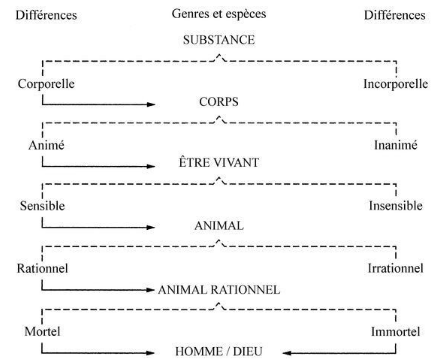
\includegraphics[width=12cm]{images/arbre_porprhyre_differences.png}
	\caption[Arbre porphyrien prenant en compte les différences]{Arbre porphyrien prenant en compte les différences [Source: \cite[chap.1]{eco_arbre_2010}]}
	\label{arbre_porphyre_differences}
\end{figure}

Cependant, si la prise en compte des différences permet de différencier l'homme du cheval, elles ne permettent pas de distinguer le cheval de l'âne par exemple. Un même genre doit donc être utilisé plusieurs fois dans l'arbre, ce qui le rend infini, et l'établissement d'un dictionnaire impossible à réaliser (voir \reference{arbre_porphyre_boucle}).\\

\begin{figure}[!h]
	\centering
	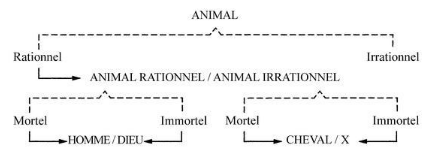
\includegraphics[width=12cm]{images/arbre_porphyre_boucle.png}
	\caption[Infinitude de l'arbre de Porphyre]{Infinitude de l'arbre de Porphyre [Source: \cite[chap.1]{eco_arbre_2010}]}
	\label{arbre_porphyre_boucle}
\end{figure}

Face à cette impossibilité de décrire le monde avec des divisions uniques dans un seul arbre, c'est à dire d'établir un dictionnaire universel, absolu et global, la seule solution paraît être la création d'un nombre d'arbres infini, composés de propriétés s'articulant selon le contexte et le domaine d'utilisation de l'arbre: d'un seul arbre insaisissable, une forêt réorganisable à l'envi et à l'infini est apparue, laissant le choix à l'utilisateur de l'arbre utilisé selon le sujet.

\subsection{\label{I-C-1-b}L'encyclopédisme (Antiquité - Moyen-Âge): la recherche d'un arbre global mimant le monde réel}
\titreEntete{L'encyclopédisme}

L'utopie de saisie totale du monde se retrouve dans l'encyclopédisme, dès l'\textit{Historia naturalis} de \nP{Pline}{l'Ancien}. Sur le même principe que l'arbre porphyrien, la hiérarchie de l'index de cette encyclopédie de 37 volumes part de l'original vers le dérivé, du naturel à l'artifice: \og Une encyclopédie, pour s’organiser, tente de suivre le modèle de l’arbre --- qui est toujours plus ou moins consciemment celui de la subdivision binaire d’un arbre porphyrien\fg{}\footnote{\cite[chap.1]{eco_arbre_2010}. Voir \reference{index_pline}}. Cependant, l'index d'une encyclopédie se distingue des termes d'un arbre porphyrien en ce qu'il est défini dans un autre développement --- un article d'encyclopédie ---, alors que les termes de l'arbre de Porphyre ne peuvent pas être définis par la suite.

\begin{figure}[!h]
	\centering
	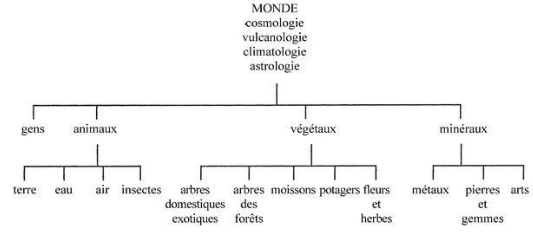
\includegraphics[width= 13cm]{images/index_pline.png}
	\caption{Extrait de l'arborescence de l'index de \nP{Pline}{l'Ancien}}
	\label{index_pline}
\end{figure}

Avec le passage au christianisme, l'encyclopédisme doit décrire les textes sacrés et non plus le monde. Ainsi, des éléments moralisateurs et allégoriques se retrouvent dans les index, devant les éléments matériels du monde\footnote{La tradition moralisatrice encyclopédique naît avec le \textit{Physiologos} d'un auteur grec et s'inspire de l'œuvre de \nP{Pline}{l'Ancien}, et se poursuit tout au long du Moyen-Âge avec les \textit{Étymologies} d'\nP{Isidore}{de Séville} notamment.}. À partir du \textsc{XIII}\textsuperscript{ème}siècle, les encyclopédies montrent l'ordre qui les dirige: cela conduit à \textit{L'arbre de science} de \nP{Raymond}{Lulle} qui créé seize arbres représentant l'Être, chacun représentant un savoir différent en se divisant en sept parties (racines, tronc, branches, rameaux, feuilles, fleurs, fruits)\footcite[chap.10]{eco_arbre_2010}. Contrairement à l'arbre de Porphyre qui est un arbre vide que l'on peut remplir selon le contexte, les arbres que propose \nP{Raymond}{Lulle} sont pleins et ont pour vocation de décrire et de classer le monde, la Grande Chaîne de l'Être.

\subsection{\label{I-C-1-c}Influences: une diversité de référentiels hiérarchiques}
\titreEntete{Influences: une diversité de référentiels hiérarchiques}

La pensée aristotélicienne puis le commentaire porphyrien ont produit une tradition de hiérarchisation du monde qui s'est poursuivie pendant plus d'un millénaire, sans cesse confrontée à l'impossibilité d'une description totale de ce monde. La multiplicité des arbres est, chez \nP{Umberto}{Eco} puis dans celle de \nP{Raymond}{Lulle}, la conclusion de leur réflexion. L'influence de cette tradition de description est sensible jusqu'à aujourd'hui, notamment dans le domaine de l'indexation et de la bibliothéconomie.\\

En effet, une diversité de référentiels est apparue, chacun étant dérivé d'un arbre. Des schémas de classification sont définissables à l'infini, emboîtant les genres, les espèces et les différences\footnote{\og Un simple artifice classificatoire consiste à emboîter des genres, des espèces et des différences sans en expliquer le \textit{definiendum}\fg{} in \cite[chap.1]{eco_arbre_2010}}. La taxonomie naît de ce modèle d'arbre: la taxonomie n'a pas pour but de dire comment repérer le concept décrit, elle permet seulement de classer en renvoyant, pour chaque nœud, vers un autre chapitre où l'on décrit ces propriétés. La taxonomie, bien qu'historiquement appliquée aux sciences de la terre, a été reprise par \nP{Melvil}{Dewey} dans sa classification décimale \index[referentiels]{dewey@Dewey} en 1876.\\

Définie comme un \og classement hiérarchique de termes préférentiels\fg{} par \nP{Louis}{Rosenfeld} et \nP{Peter}{Morville}\footcite{rosenfeld_information_2015}, la taxonomie ne veut pas définir, mais simplement permettre l'utilisation correcte et logique du terme par l'attribution de catégories et l'utilisation exclusive de relations hiérarchiques.\\

Les \textit{thesauri}\footnote{Ils sont décrits comme une \og liste organisée de termes contrôlées et normalisés (descripteurs et non-descripteurs) servant à l’indexation des documents et des questions dans un système documentaire\fg{} dans \cite{degez_thesauroglossaire_2001}. Peu formels, ils sont néanmoins le vocabulaire le plus utilisé pour l'indexation. L'un des \textit{thesauri} les plus utilisés est le \ac{gemet}(\cite{noauthor_general_nodate}). Le \index[referentiels]{gemet@GEMET} est disponible en plus de trente langues et diffusé par l'Agence européenne de l'Énergie. Voir \reference{I-C-2}.} utilisent plus de relations et de types de termes, de manière à indexer des contenus avec des mots-clés et à faciliter la recherche. Ce vocabulaire contrôlé hiérarchique reste proche du langage naturel en y intégrant les variantes, les synonymes, les descriptions, les traductions et les équivalences.\\

Pour avoir une plus grande formalisation du thésaurus, il faut utiliser une ontologie. Cette ontologie est la spécification formelle d'un espace de noms, d'un domaine particulier de la connaissance\footnote{L'une des ontologies les plus utilisées, notamment dans le web sémantique, est \ac{foaf}. \index[referentiels]{foaf@FOAF} permet la description précise des personnes. Voir \cite{noauthor_foaf_nodate}}. Elle identifie alors les objets à décrire, leurs relations au sein de ce domaine ainsi que leurs propriétés. L'ontologie n'est pas utilisée directement dans l'indexation ou la recherche, elle est d'abord utilisée pour instancier et raisonner, en s'éloignant du langage naturel avec l'utilisation d'identifiants techniques.\\

Les taxonomies, les \textit{thesauri} ainsi que les ontologies héritent tous du modèle de l'arbre, la description ou la classification par la hiérarchie étant la plus efficace pour ces besoins. Ces vocabulaires sont les plus complexes par les relations qui les composent. \nP{Louis}{Rosenfeld} et \nP{Peter}{Morville}\footnote{\cite{rosenfeld_information_2015}. Voir \reference{frise_voca}} considèrent l'anneau de synonymie comme le plus simple des vocabulaires, avec des relations d'équivalence, alors que les fichiers d'autorité et les taxonomies, fonctionnant sur la hiérarchie, sont plus complexes. Les \textit{thesauri} et les ontologies sont plus complexes encore puisqu'ils sont constitués de relations hiérarchiques et associatives.

\begin{figure}[!h]
	\centering
	
	\begin{pspicture}(0,2)(10,8)
		\psline[linewidth=1.5pt]{->}(0,5)(10,5)
		\uput[0](-2.5,5){\textsc{Simple}}
		\uput[0](10.5,5){\textsc{Complexe}}
		\uput[0](3,3){\textbf{\textsc{Type de relations}}}
		\uput[0](2.5,7){\textbf{\textsc{Type de vocabulaire}}}
		\uput[0](0,4){Équivalence}
		\uput[0](3.8,4){Hiérarchique}
		\uput[0](7.6,4){Associative}
		\uput[0](-1,6.3){Anneau de synonymie}
		\uput[0](2.5,5.5){Fichiers d'autorité}
		\uput[0](5,6.1){Taxonomies}
		\uput[0](7,5.5){Thésaurus}
		\uput[0](9,6.3){Ontologies}
	\end{pspicture}
	
	\caption[Classification des vocabulaires selon leur complexité]{Classification des vocabulaires selon leur complexité [d'après \cite{rosenfeld_information_2015}]}
	\label{frise_voca}
\end{figure}

\section{\label{I-C-2}Le \textit{thésaurus}, vocabulaire contrôlé hiérarchique le plus fréquent}
\titreEntete{Le thésaurus}

Né dans les années 1950 aux États-Unis, le \index[ref]{typologie@Typologie!thesaurus@Thésaurus}thésaurus n'a été adopté massivement qu'avec l'apparition de l'informatique. C'est un langage combinatoire, une liste organisée de termes normalisés et contrôlés, qui permet de faire le lien entre le langage naturel de l'homme et le nécessaire besoin d'avoir un langage contrôlé pour les ressources. La sélection d'un terme lors de l'indexation permet de sélectionner un concept lui-même décrit par plusieurs termes (synonymes, équivalents, traductions). Ainsi, les institutions patrimoniales se sont emparées de cet outil, adaptable au domaine de chacune: l'\ac{ina} possède un thésaurus orienté vers l'audiovisuel, la Cinémathèque française un \href{http://www.cineressources.net/thesaurus/}{thésaurus orienté vers le cinéma}.

\subsection{\label{I-C-2-a}Types de structure}
\titreEntete{Types de structure}

Le type de \index[ref]{typologie@Typologie!thesaurus@Thésaurus}thésaurus le plus utilisé est celui constitué d'une hiérarchie simple\footnote{La typologie des \textit{thesauri} décrite par la suite est présente chez \cite{rosenfeld_information_2015}.}. L'\ac{ina} possède un thésaurus de noms communs formé sur cette hiérarchie simple à unique ascendance\footnote{Voir \reference{annexe_thesaurus}}, c'est à dire qu'un terme est nécessairement descendant d'une seule classe, il ne peut pas hériter de deux caractéristiques différentes, ce qui le rapproche de la \index[ref]{typologie@Typologie!taxonomie@Taxonomie}taxinomie\footnote{Voir \reference{modele_taxo} et \reference{modele_thes_simple}.}.

\begin{figure}[!h]
	\begin{minipage}[c]{.46\linewidth}
			\centering
			\begin{pspicture}(0,2.5)(6.5,7)
				\psframe[fillstyle=solid,fillcolor=lightgray](0,6)(1.5,6.5)
				\psframe[fillstyle=solid,fillcolor=lightgray](1.5,5)(3,5.5)
				\psframe[fillstyle=solid,fillcolor=lightgray](3,4)(4.5,4.5)
				\psframe[fillstyle=solid,fillcolor=lightgray](4.5,3)(6,3.5)
				\psline{->}(0.75,6)(0.75,5.2)(1.5,5.2)
				\psline{->}(2.25,5)(2.25,4.2)(3,4.2)
				\psline{->}(3.75,4)(3.75,3.2)(4.5,3.2)
			\end{pspicture}
			\caption{Le modèle taxonomique}
			\label{modele_taxo}
	\end{minipage}
	\begin{minipage}[c]{.46\linewidth}
			\centering
			\begin{pspicture}(0,1.5)(7,7)
			\psframe[fillstyle=solid,fillcolor=lightgray](3,6.5)(4.5,7)
			\psline{->}(3.75,6.5)(3.75,5.5)
			\psframe[fillstyle=solid,fillcolor=lightgray](3,5)(4.5,5.5)
			\psline(3.75,5)(3.75,4.5)
			\psframe[fillstyle=solid,fillcolor=lightgray](1.5,3.5)(3,4)
			\psline{->}(3.75,4.5)(2.25,4.5)(2.25,4)
			\psframe[fillstyle=solid,fillcolor=lightgray](4.5,3.5)(6,4)
			\psline{->}(3.75,4.5)(5.25,4.5)(5.25,4)
			\psframe[fillstyle=solid,fillcolor=lightgray](0.75,2)(2.25,2.5)
			\psline{->}(2.25,3.5)(2.25,3)(1.5,3)(1.5,2.5)
			\psline(5.25,3.5)(5.25, 3)
			\psframe[fillstyle=solid,fillcolor=lightgray](3.5,2)(5,2.5)
			\psline{->}(5.25, 3)(4.25,3)(4.25,2.5)
			\psframe[fillstyle=solid,fillcolor=lightgray](5.5,2)(7,2.5)
			\psline{->}(5.25, 3)(6.25,3)(6.25,2.5)
			\end{pspicture}
			\caption{Le modèle du thésaurus simple}
			\label{modele_thes_simple}
	\end{minipage}
	\medskip
	\\
	\caption*{Comparaison entre le modèle taxonomique et celui du thésaurus à hiérarchie simple [d'après \cite{rosenfeld_information_2015}]}
\end{figure} 

De manière à exprimer la descendance depuis plusieurs caractéristiques, un thésaurus polyhiérarchique existe. Il permet de définir et d'accepter plus de termes contrôlés que le thésaurus simple. En effet, par la combinaison des termes ascendants, un même terme peut avoir deux ascendances différentes. \nP{Peter}{Morville} et \nP{Louis}{Rosenfeld} prennent un exemple médical pour illustrer ce type particulier de thésaurus.

\begin{figure}[!h]
	\begin{minipage}[c]{.46\linewidth}
			\centering
			\begin{pspicture}(0,1.75)(7,8.75)
			\psframe[fillstyle=solid,fillcolor=lightgray](1.5,8)(3,8.5)
			\psline{->}(3.75,7.5)(3.75,7)
			\psline(3.75,7.5)(2.25,7.5)(2.25,8)
			\psframe[fillstyle=solid,fillcolor=lightgray](4.5,8)(6,8.5)
			\psline(3.75,7.5)(5.25,7.5)(5.25,8)
			\psframe[fillstyle=solid,fillcolor=lightgray](3,6.5)(4.5,7)
			\psline{->}(3.75,6.5)(3.75,5.5)
			\psframe[fillstyle=solid,fillcolor=lightgray](3,5)(4.5,5.5)
			\psline(3.75,5)(3.75,4.5)
			\psframe[fillstyle=solid,fillcolor=lightgray](1.5,3.5)(3,4)
			\psline{->}(3.75,4.5)(2.25,4.5)(2.25,4)
			\psframe[fillstyle=solid,fillcolor=lightgray](4.5,3.5)(6,4)
			\psline{->}(3.75,4.5)(5.25,4.5)(5.25,4)
			\psframe[fillstyle=solid,fillcolor=lightgray](0.75,2)(2.25,2.5)
			\psline{->}(2.25,3.5)(2.25,3)(1.5,3)(1.5,2.5)
			\psline(5.25,3.5)(5.25, 3)
			\psframe[fillstyle=solid,fillcolor=lightgray](3.5,2)(5,2.5)
			\psline{->}(5.25, 3)(4.25,3)(4.25,2.5)
			\psframe[fillstyle=solid,fillcolor=lightgray](5.5,2)(7,2.5)
			\psline{->}(5.25, 3)(6.25,3)(6.25,2.5)
			\end{pspicture}
			\caption{Le modèle polyhiérarchique}
			\label{modele_polyh}
		\end{minipage}
	\begin{minipage}[c]{.46\linewidth}
	\centering
	\begin{pspicture}(0,1.75)(5,6)
		\psframe[fillstyle=solid,fillcolor=lightgray](1.75,5)(3.25,5.5)
		\psline(2.5,5)(2.5,4.5)
		\uput[0](1.75,5.25){Décès}
		\psframe[fillstyle=solid,fillcolor=lightgray](0.75,3.5)(2.25,4)
		\psline{->}(2.5,4.5)(3.5,4.5)(3.5,4)
		\uput[0](0.75,3.75){Virus}
		\psframe[fillstyle=solid,fillcolor=lightgray](2.75,3.5)(4.25,4)
		\psline{->}(2.5,4.5)(1.5,4.5)(1.5,4)
		\uput[0](2.6,3.75){\scriptsize{Respiration}}
		\psframe[fillstyle=solid,fillcolor=lightgray](1.75,2)(3.25,2.5)
		\uput[0](1.6,2.25){\scriptsize{Pneumonie}}
		\psline(1.5,3.5)(1.5,3)(2.5,3)
		\psline(3.5,3.5)(3.5,3)(2.5,3)
		\psline{->}(2.5,3)(2.5,2.5)
	\end{pspicture}
	\caption{Application du modèle polyhiérarchique}
	\label{application_polyh}
\end{minipage}
\medskip
\\
\caption*{Le modèle du thésaurus polyhiérarchique [d'après \cite{rosenfeld_information_2015}]}
\end{figure}

Enfin, comme nous l'avons évoqué précédemment\footnote{Voir \reference{I-C-1}.}, le seul arbre possible est un arbre multiple, adapté à son contexte. Ainsi, des \textit{thesauri} à facettes existent, reflétant les multiples dimensions thématiques que peuvent contenir les documents ou les éléments: un terme se retrouve alors dans plusieurs arbres, multipliant les points d'accès. Plusieurs \index[ref]{typologie@Typologie!thesaurus@Thésaurus}\textit{thesauri} simples sont par conséquent créés, permettant la description de l'ensemble de ces dimensions.

\subsection{\label{I-C-2-b}Relations entre les termes}
\titreEntete{Relations entre les termes}

La force du \index[ref]{typologie@Typologie!thesaurus@Thésaurus}thésaurus ne réside pas seulement dans l'enchaînement d'ascendances et de descendances. Les relations établies entre les termes sont essentielles pour permettre le lien entre le langage humain naturel et le besoin de contrôle imposé par l'indexation et la recherche: un thésaurus est \og un vocabulaire contrôlé dans lequel les relations d'équivalence, de hiérarchie et d'association sont correctement identifiées de manière à permettre une meilleure récupération\fg{}\footcite{rosenfeld_information_2015}.\\

Les relations créées précisent le sens de chaque vedette par comparaison aux vedettes de sens voisin, elles permettent de naviguer entre ces vedettes pour affiner sa recherche, l'élargir ou bien la réorienter. La hiérarchisation et l'établissement de liens permettent de passer à une navigation sémantique, alors que les simples vocabulaires contrôlés évoqués au \reference{I-A} ne permettaient qu'une navigation par mots.\\

La première relation est la relation d'équivalence.
\begin{wrapfigure}{L}{4cm}
	\centering
	\begin{pspicture}(0,0)(2.6,2.6)
	\pscircle(1.3,1.3){1.3}
	\uput[0](0.5,1.3){A~=~B}
\end{pspicture}
	\caption{Relation d'équivalence}
	\label{relation_equivalence}	
\end{wrapfigure} Elle connecte le terme préférentiel --- le terme principal de la vedette --- à ses variantes: les synonymes, les acronymes, les abréviations, les variantes lexicales ou les différences de graphie sont ainsi incorporés au thésaurus comme variantes. Cette relation\footnote{Voir \reference{relation_equivalence}} est une relation horizontale, d'égalité, comme dans l'anneau de synonymie. Dans l'\reference{annexe_thesaurus}, le terme \og Cadreur\fg{}, qui est le terme préférentiel, a deux variantes --- ou termes \og Employés pour\fg{}, \og Cameraman\fg{} et \og Opérateur de prise de vue\fg{}.\\

Le second type de relation est la relation associative. \begin{wrapfigure}{R}{5cm}
	\centering
	\begin{pspicture}(0,0)(4.6,2.6)
	\pscircle(1.3,1.3){1.3}
	\uput[0](0.6,1.3){A}
	
	\pscircle(3.2,1.3){1.3}
	\uput[0](3,1.3){B}
\end{pspicture}
	\caption{Relation d'association}
	\label{relation_association}	
\end{wrapfigure} Comme la relation d'équivalence, elle est horizontale. Elle permet d'exprimer la proximité sémantique entre deux termes: dans \index[ref]{lod@Linked Open Data (LOD)!rameau@RAMEAU}\index[ref]{autorites@Autorités!rameau@RAMEAU}\ac{rameau}, la vedette \href{https://data.bnf.fr/fr/11933646/television/}{\og Télévision\fg{}} possède quarante relations d'association avec d'autres vedettes, comme \href{https://data.bnf.fr/fr/12648926/industrie_de_la_television/}{\og Industrie de la télévision\fg{}}. L'association\footnote{Voir \reference{relation_association}.} n'est pas une relation de stricte égalité, elle indique le partage sémantique d'une partie de leur définition. Cette relation permet l'élargissement d'une recherche depuis une vedette.\\

Le dernier type de relation est hiérarchique. Il est le plus utilisé car il permet l'expression de nombreuses relations du langage naturel: \begin{wrapfigure}{L}{5cm}
	\centering
	\begin{pspicture}(0,0)(2.6,2.6)
	\pscircle(1.3,1.3){1.3}
	\uput[0](0.6,1.6){A}
	
	\pscircle(1.5,1){0.5}
	\uput[0](1.1,1){B}
\end{pspicture}
	\caption{Relation de hiérarchie}
	\label{relation_hierar}	
\end{wrapfigure}
\begin{itemize}
	\item la relation génétique --- la plus fréquente --- peut ainsi être exprimée. Le sens du terme générique est inclus dans celui du terme spécifique: la vedette \index[ref]{lod@Linked Open Data (LOD)!rameau@RAMEAU}\index[ref]{autorites@Autorités!rameau@RAMEAU}\ac{rameau} \href{https://data.bnf.fr/fr/11960499/radiodiffusion/}{\og Radiodiffusion\fg{}} est l'un des termes génériques de  \href{https://data.bnf.fr/fr/11933646/television/}{\og Télévision\fg{}} qui est elle-même terme générique de \href{https://data.bnf.fr/fr/11936935/chaines_de_television/}{\og Chaînes de télévision\fg{}} notamment. Chacune de ces vedettes est décrite par son ascendance et sa descendance.
	\item la relation d'appartenance --- ou de regroupement --- est possible;
	\item la relation partitive
\end{itemize}
La définition de cette relation hiérarchique\footnote{Voir \reference{relation_hierar}.} permet l'expression de caractéristiques et de relations infinies du langage naturel. La recherche d'une vedette peut alors être affinée --- quand l'utilisateur passe d'une vedette générique à une vedette spécifique --- ou bien élargie --- quand il passe d'une vedette spécifique à une vedette générique.\\

Alors, chaque terme devient le centre de son propre réseau et construit un nouvel arbre, entièrement né de son contexte.


\subsection{\label{I-C-2-c}Utiliser la précoordination pour les relations complexes}
\titreEntete{Utiliser la précoordination pour les relations complexes}

L'inconvénient du \index[ref]{typologie@Typologie!thesaurus@Thésaurus}thésaurus comme évoqué précédemment est l'impossibilité pour l'utilisateur de feuilleter \index[ref]{typologie@Typologie!index@Index}l'index: \og Télévision\fg{} et \og Chaînes de télévision\fg{}, bien qu'étant proches, ne seraient pas au même endroit dans l'index. Pour faciliter la navigation de l'utilisateur, les mots-clés sont coordonnés avant l'utilisation par l'utilisateur pour former une vedette-matière construite (comme dans le cas de \index[ref]{lod@Linked Open Data (LOD)!rameau@RAMEAU}\index[ref]{autorites@Autorités!rameau@RAMEAU}\ac{rameau}): une vedette principale constitue la tête de la vedette, puis des subdivisions la complètent\footnote{Dans \og \href{https://data.bnf.fr/fr/11977461/plantes-hotes/}{Plantes -- Parasites -- Plantes-hôtes}\fg{}, \og Plantes\fg{} est la tête de vedette, complétée par deux subdivisions.}. Une vision globale est ainsi offerte et permet une précision du sujet des facettes ainsi qu'une limitation du bruit: \href{https://data.bnf.fr/fr/11977461/plantes-hotes/}{Plantes -- Parasites -- Plantes-hôtes}\fg{} est ainsi séparée de \href{https://data.bnf.fr/fr/12397201/plantes_parasites/}{\og Plantes parasites\fg{}}.\\

\bigskip
\bigskip
Les différentes structures de \index[ref]{typologie@Typologie!thesaurus@Thésaurus}\textit{thesauri} et leurs multiples relations permettent un modèle de classification, de combinaison et de description efficace des termes, à la fois proche du langage naturel mais en s'en éloignant par le formalisme et le contrôle des termes. Chaque vedette est le centre de son propre référentiel, dirigeant vers des variantes, des vedettes proches ou en relation.

\begin{figure}[!h]
	\centering
	
	\begin{pspicture}(0,0)(15,7.6)
		\psline{->}(7.5,3)(7.5,3.5)
		\psframe[fillstyle=solid,fillcolor=lightgray](0,0)(3,1)
		\uput[0](0.8,0.8){Terme}
		\uput[0](0.9,0.3){relatif}
		\psline{->}(1.5,2)(1.5,1)
		\uput[0](0.3,2.8){Relation d'}
		\uput[0](0.3,2.3){association}
		\psline(2.5,3)(7.5,3)
		\psframe[fillstyle=solid,fillcolor=lightgray](6,0)(9,1)
		\uput[0](6.8,0.8){Terme}
		\uput[0](6.5,0.3){spécifique}
		\psline{->}(7.5,1.5)(7.5,1)
		\uput[0](6.6,2.3){Relation}
		\uput[0](6.3,1.8){hiérarchique}
		\psline(7.5,3)(7.5,2.5)
		\psframe[fillstyle=solid,fillcolor=lightgray](12,0)(15,1)
		\uput[0](12.8,0.8){Terme}
		\uput[0](12.9,0.3){relatif}
		\psline{->}(13.5,2)(13.5,1)
		\uput[0](12.5,2.8){Relation d'}
		\uput[0](12.3,2.3){association}
		\psline(12,3)(7.5,3)
		
		\psframe[fillstyle=solid,fillcolor=lightgray](0,3.5)(3,4.5)
		\uput[0](0.5,4){Variante}
		\psline{->}(3.5,4)(3,4)
		\uput[0](3.5,4.2){Relation d'}
		\uput[0](3.5,3.8){équivalence}
		\psline{->}(5.5,4)(6,4)
		\psframe[fillstyle=solid,fillcolor=lightgray](6,3.5)(9,4.5)
		\uput[0](6.8,4.2){Terme}
		\uput[0](6.5,3.8){préférentiel}
		\psframe[fillstyle=solid,fillcolor=lightgray](12,3.5)(15,4.5)
		\uput[0](12.5,4){Variante}
		\psline{->}(9.5,4)(9,4)
		\uput[0](9.5,4.2){Relation d'}
		\uput[0](9.5,3.8){équivalence}
		\psline{->}(11.5,4)(12,4)
		
		\psframe[fillstyle=solid,fillcolor=lightgray](6,6.5)(9,7.5)
		\uput[0](6.8,7.2){Terme}
		\uput[0](6.5,6.7){générique}
		\psline{->}(7.5,5)(7.5,4.5)
		\psline{->}(7.5,6)(7.5,6.5)
		\uput[0](6.6,5.6){Relation}
		\uput[0](6.3,5.2){hiérarchique}
	\end{pspicture}
	\caption[Modélisation d'une vedette de thésaurus]{Modélisation d'une vedette de thésaurus [d'après \cite{rosenfeld_information_2015}]}
	\label{modelisation_thes}
\end{figure}

\section[Passer du texte libre à un vocabulaire contrôlé: aligner des notes qualités et un thésaurus de noms communs]{\label{I-C-3}Passer du texte libre à un vocabulaire contrôlé}
\titreEntete{Passer du texte libre à un vocabulaire contrôlé}

Dans la description de documents audiovisuels --- comme dans celle d'autres documents patrimoniaux ---, désigner des personnes est indispensable. Pour enrichir le seul état civil de la personne, plusieurs moyens peuvent être utilisés:
\begin{itemize}
	\item rédiger un texte libre décrivant les caractéristiques de la personne, ses fonctions, ses dates de naissance et de mort, \dots. Cette solution pose la problématique de la structuration des données: un texte libre n'est pas lisible par une machine; son accès est par conséquent restreint.
	\item utiliser un \index[ref]{typologie@Typologie!vocabulaires controles@Vocabulaires contrôlés}vocabulaire contrôlé et sélectionner les termes correspondant à la personne. Cependant, en fonction du niveau de précision souhaité, ce vocabulaire doit être plus ou moins précis, rendant, dans le cas d'une grande précision, la description longue et fastidieuse.
	\item définir des champs essentiels à la description de cette personne, et rédiger un texte libre pour les informations supplémentaires. De même que dans le premier cas, le texte libre appauvrit l'effort de structuration de la description.
\end{itemize}
Face à ces difficultés, les documentalistes de la \ac{ddcol} à l'\ac{ina} ont créé des vedettes de personnes selon une succession de champs (sexe, date de naissance, date de mort, \dots) et de notes, dont une note qualité qui est régie par un guide de rédaction. Cette note qualité a pour but de décrire en quelques mots les fonctions de la personne et le lieu d'exercice. Cette note n'étant pas un point d'accès, elle peut être structurée et rédigée en texte libre.\\

Dans le cadre de la migration des données de la \ac{ddcol} dans le \ldd, un alignement de ces notes qualités est nécessaire avec le \index[ref]{typologie@Typologie!thesaurus@Thésaurus}thésaurus des noms communs qui existe parallèlement, notamment pour enrichir le thésaurus des fonctions des notes qualités qui n'y existent pas.

\subsection{\label{I-C-3-a}Contrôler du texte libre}
\titreEntete{Contrôler du texte libre}

La note qualité est rédigée selon des règles définies au préalable par les documentalistes. Cependant, la rédaction en texte libre conduit à l'apparition d'erreurs humaines, comme les erreurs de graphie, de grammaire ou de ponctuation. En effet, une note qualité peut avoir deux formes:
\begin{itemize}
	\item Fonction1, fonction2, \dots~. Pays
	\item Homonymes: 1 - Fonction1, fonction2, \dots~. Pays1, Pays2, \dots; 2 - Fonction1, fonction2, \dots~. Pays 
\end{itemize}
Ainsi, l'oubli d'une ponctuation, ou son inversion, conduit à rendre la note qualité non conforme aux règles et, par conséquent, à rendre son traitement plus difficile voire impossible. De plus, les différences de graphie liées au masculin et au féminin, ainsi qu'au singulier et au pluriel, rendent ces notes qualités très différentes.\\

De manière à pouvoir les aligner avec le \index[ref]{typologie@Typologie!thesaurus@Thésaurus}thésaurus des noms communs, un premier traitement est nécessaire, pour extraire et normaliser les fonctions. Le logiciel ETL (\textit{Extract Transform Loaad})\footnote{Un ETL permet de migrer des données depuis une source vers une cible, en leur appliquant des traitements avant de les charger dans la cible.} \href{https://www.talend.com/fr/products/big-data/}{Talend Big Data Platform} permet ce premier traitement.\\

La première étape consiste à scinder chaque note selon les fonctions et les pays: le point sépare ces deux éléments et permet cette scission. Ainsi, la fonction extraite de \og Historien, musicologue. France\fg{} est \og Historien, musicologue\fg{} alors que la note qualité \og Journaliste, France\fg{} ne peut pas être scindée correctement. Une seconde scission intervient par la suite de manière à récupérer chaque fonction une à une, passant de \og Historien, musicologue\fg{} à \og Historien\fg{} et \og musicologue\fg{}.\\

Quand les fonctions sont récupérées, le contrôle des termes peut avoir lieu selon plusieurs choix à effectuer en amont:
\begin{itemize}
	\item le choix du genre doit être effectué pour éviter les termes équivalents dans le sens mais différents en graphie
	\item le choix du nombre
	\item la gestion de la ponctuation propre aux fonctions comme les traits d'union
	\item la gestion de l'accentuation
\end{itemize}
Pour normaliser le plus possible, le choix du masculin singulier, de la suppression de toute la ponctuation et de l'accentuation ont été effectué. Pour les choix du genre, le nombre des exceptions comme \og musée\fg{}, portant une terminaison du féminin, étant plus faible que le nombre de tous les féminins, le choix du masculin s'est imposé pour normaliser le maximum de fonctions. La \autoref{exemple_realisateur_NQ} montre une dernière normalisation à effectuer: la suppression des \textit{stopwords}, effectuée en \autoref{exemple_realisateur_NQ2}.
\begin{table}[!h]
	\centering
	\csvautotabular[separator=semicolon]{images/dessinateur_fonctions.csv}
	\caption{Données d'exemple de notes qualités avec la fonction de Réalisateur}
	\label{exemple_realisateur_NQ}
\end{table}
\begin{table}[!h]
	\centering
	\csvautotabular[separator=semicolon]{images/dessinateur_fonctions2.csv}
	\caption{Données d'exemple de notes qualités avec la fonction de Réalisateur, après normalisation des fonctions}
	\label{exemple_realisateur_NQ2}
\end{table}
\bigskip

Après la normalisation, les fonctions sont suffisamment contrôlées et proches des règles d'un \index[ref]{typologie@Typologie!thesaurus@Thésaurus}thésaurus pour être alignées. Cependant, nous pouvons observer que les erreurs humaines de graphie, comme l'oubli d'un \og s\fg{} dans \og dessinateur\fg{}, restent et ne permettront pas, par conséquent, d'être alignées. Le traitement correct de l'ensemble des notes en texte libre reste impossible suite aux erreurs introduites par l'homme.\\

Enfin, les notes qualités de l'\ac{ina} comprennent également des qualités ne décrivant pas directement la personne, mais définissant cette personne par un lien avec un fait. C'est le cas des faits divers, des attentats, des affaires judiciaires dans lesquels une personne peut être impliquée comme victime, accusée, témoin, \dots; c'est le cas également des indications de filiation et de généalogie avec lesquelles une personne est seulement désignée, sans apporter de précisions sur ses véritables fonctions\footnote{Voir \reference{exemple_NQ_sans_fonctions}.}. Ces parties de notes qualités --- ou bien la totalité de ces notes --- ne décrivant pas la fonction de la personne et n'allant pas trouver d'équivalent dans le \index[ref]{typologie@Typologie!thesaurus@Thésaurus}thésaurus, elles sont écartées du traitement.
\begin{table}[!h]
	\centering
	\csvautotabular[separator=semicolon]{images/affaires_attentat.csv}
	\caption{Données d'exemple de notes qualités sans fonctions}
	\label{exemple_NQ_sans_fonctions}
\end{table}

\subsection{\label{I-C-3-b}Aligner les extractions en langage naturel avec un thésaurus de noms communs}
\titreEntete{Aligner avec un thésaurus de noms communs}

Avec le premier traitement de normalisation des fonctions, les notes qualités sont sorties du langage naturel de manière à pouvoir être contrôlées dans un vocabulaire plus strict. L'alignement avec le \index[ref]{typologie@Typologie!thesaurus@Thésaurus}thésaurus de noms communs peut alors être réalisé\footnote{De manière à avoir la même normalisation de chaque côté de l'alignement, le thésaurus a subi le même traitement que les notes qualité, avec l'application des mêmes règles.}. Ce thésaurus est classé dans un ordre hiérarchique, mais l'accès par des termes ascendants est difficile pour l'alignement: les termes génériques sont souvent des noms qui ne sont pas des fonctions, ce qui rend leur alignement impossible. Ainsi, le terme \og Dessinateur\fg{} a pour ascendance \og \$art et culture/arts plastiques/dessin\fg{}: \og Dessin\fg{} ou \og Arts plastiques\fg{} ne sont pas des fonctions. L'ensemble des alignements est par conséquent réalisé avec les termes préférentiels les plus bas dans l'arborescence. Le thésaurus contenant également des synonymes\footnote{Voir les termes \textit{Employés pour} dans l'\reference{annexe_thesaurus} (\reference{thesaurus_cadreur}).}, ces derniers sont utilisés dans l'alignement de manière à réduire encore l'impact du langage naturel des notes qualités sur la qualité de l'alignement.\\

Cette phase d'alignement est également réalisée avec Talend grâce à une succession de jointures\footnote{Ici, les jointures sont des \textit{inner join} pour aligner sur la similarité entre les deux côtés --- fonctions issues de la note qualité, et termes du thésaurus --- , ou bien des comparaison effectuées à partir du début de la fonction issue des notes qualités --- \og Illustrateur de presse\fg{} pourra ainsi correspondre au terme \og Illustrateur\fg{} du thésaurus.}. Les fonctions strictement égales au terme préférentiel du thésaurus sont ainsi alignées, ainsi que celles qui commencent par un terme du thésaurus. Cette étape de l'alignement montre les difficultés posées par l'utilisation du texte libre dans la description ainsi que la gestion impossible des coquilles, bien que parfois très proche du terme exact\footnote{Voir l'exemple de l'alignement du terme \og Journaliste\fg{} \reference{annexe_alignement_journaliste}.}.\\

Face à ces difficultés et au nombre peu élevé des alignements qui résultent de cette étape, l'utilisation des synonymes peut apporter des résultats supplémentaires: l'entrée \og Cuisinier\fg{} du \index[ref]{typologie@Typologie!thesaurus@Thésaurus}thésaurus de noms communs comprend un synonyme, \og Chef de cuisine\fg{}. Cependant, le nombre des synonymes est réduit, et des alignements sont ici aussi non réalisés\footnote{Voir \reference{alignement_cuisinier}}.
\begin{table}[!h]
	\centering
	\csvautotabular[separator=semicolon]{images/alignement_cuisinier.csv}
	\caption{Utilisation des synonymes pour l'alignement du terme \og Cuisinier\fg{}}
	\label{alignement_cuisinier}
\end{table}

Enfin, le cas de \og Chef cuisinier\fg{} montre la nécessité d'utiliser le second terme de l'expression de la fonction\footnote{Voir \reference{alignement_cuisinier_polysemie}}: cette dernière étape de l'alignement permet l'alignement des fonctions commençant par des termes polysémiques comme \og Chef\fg{}, \og Directeur\fg{}, \og Maître\fg{},\dots
\begin{table}[!h]
	\centering
	\csvautotabular[separator=semicolon]{images/alignement_cuisinier_polysemie.csv}
	\caption{Gestion de la polysémie dans l'alignement du terme \og Cuisinier\fg{}}
	\label{alignement_cuisinier_polysemie}
\end{table}

\subsection{\label{I-C-3-c}Classer selon le thésaurus}
\titreEntete{Classer selon le thésaurus}

L'utilisation des relations d'association a permis d'aligner les fonctions avec les termes du \index[ref]{typologie@Typologie!thesaurus@Thésaurus}thésaurus. Les relations de hiérarchie avec les termes génériques permettent de classer ces fonctions. Ainsi, elles sont utilisées pour définir huit catégories de rattachement dans les fonctions extraites des notes qualité, de manière à les classer selon le thésaurus. Dans le thésaurus des noms communs, huit termes permettent de rattacher l'ensemble des termes spécifiques, souvent avec des niveaux intermédiaires de hiérarchie\footnote{Ces huit catégories sont: \og Art et culture\fg{}, \og communication diffusion traitement information\fg{}, \og sciences\fg{}, \og sciences humaines\fg{}, \og sport\fg{}, \og vie économique\fg{}, \og vie quotidienne habitat alimentation et loisirs\fg et \og vie sociale\fg{}.}. Ces termes de catégorisation sont des facettes: ils ne sont pas attribuables directement à un concept à indexer, ils permettent le seul classement.\\

Cette opération de classement des fonctions des notes qualités selon l'arborescence du thésaurus permet, au-delà de l'ajout sémantique sur les termes alignés, de repérer les termes qui n'ont pas été alignés et d'en comprendre les raisons:
\begin{itemize}
	\item Des noms communs ne correspondant pas à des fonctions sont présents dans les notes qualité. Ainsi, des termes comme \og cirque pinder\fg{} ou \og clip
	\fg{} ne trouveront pas d'équivalence dans le thésaurus.
	\item Des noms trop spécifiques ne sont également pas présents: \og chemisier\fg{} est une fonction spécifique que les documentalistes pourront créer si nécessaire grâce à ce repérage dans les notes qualité.
	\item Des erreurs introduites par accident par l'homme empêchent certains alignements: c'est le cas par exemple de \og chercher\fg{} qui a un équivalent \og chercheur\fg{} dans le thésaurus. Il est difficile de repérer et de corriger ces erreurs automatiquement.
	\item La présence d'une documentation d'aide au catalogage et à l'indexation permet d'introduire de nouvelles règles dans la classification automatique: ainsi, \og designer interieur\fg{} peut être classifié dans la facette \og Art et culture\fg{} car la documentation l'indique; cependant, le terme \og designer\fg{} étant absent du \index[ref]{typologie@Typologie!thesaurus@Thésaurus}thésaurus, il ne peut pas être aligné.
\end{itemize}



%conclu
\bigskip
\bigskip
\bigskip
Aligner du texte libre avec un thésaurus nécessite plusieurs étapes et la prise en compte des différences de langage --- l'un étant un contrôle minimal du langage humain naturel, l'autre un vocabulaire contrôlé natif --- :
\begin{itemize}
	\item normaliser chaque côté de l'alignement selon les mêmes règles
	\item aligner selon l'exactitude avec le terme préférentiel
	\item aligner selon l'exactitude avec une variante du terme préférentiel
	\item aligner selon l'exactitude du commencement de la fonction avec le terme préférentiel
	\item aligner selon l'exactitude du commencement de la fonction avec une variante du terme préférentiel
	\item aligner selon l'exactitude du deuxième terme non polysémique de la fonction avec le terme préférentiel
\end{itemize}
	\chapter{\label{I-B}Les référentiels à l’INA}
\titreEntete{Les référentiels à l’INA}
	
	Le référentiel, tel que présenté dans les chapitres précédents, n'a pour destination que l'institution qui l'a créé, dans un unique but qui est de répondre à ses propres besoins selon ses activités. Cependant, nous l'avons évoqué, une même institution peut disposer de plusieurs référentiels, parfois similaires mais structurés différemment. Ces référentiels prennent la forme de liste de termes, ou de \textit{thesauri}, qui offrent des clés et des termes normalisés aux documents décrits. L'interopérabilité entre les bases de données n'est pas recherchée, comme celle avec des référentiels externes: le lien n'apparaît pas encore comme essentiel.\\
	
	Ainsi, le référentiel comme fournisseur de clés et de termes contrôlés n'a qu'un usage interne et spécifique; il n'est pas utilisable autre part comme le montre la \reference{schema_general_controler}.
	\begin{figure}[!h]
	\centering
	
	\begin{pspicture}(0,0)(14,7)		
		\uput[0](0.8,6.4){Entrepôt de documents A}
		\uput[0](7.8,6.4){Entrepôt de documents B}
		%cercles globaux
		\pscircle(3,3){3}
		\pscircle(10,3){3}
		%cercles du A
		\pscircle(4.8,3.4){0.6}
		\pscircle(3,4.2){0.6}
		\pscircle(1.5,3.2){0.6}
		\pscircle(2.2,1.6){0.6}
		\pscircle(3.8,1.4){0.6}
		%cercles du B
		\pscircle(9.2,3.9){0.6}
		\pscircle(11.4,2.8){0.6}
		\pscircle(9.2,1.6){0.6}
		%labels du A
		\uput[0](2.6,4.2){D1}
		\uput[0](3.4,1.4){D2}
		\uput[0](1,3.2){D3}
		\uput[0](4.4,3.4){R1}
		\uput[0](1.7,1.6){R2}
		%labels du B
		\uput[0](8.8,1.6){D1}
		\uput[0](10.9,2.8){D2}
		\uput[0](8.8,3.9){R1}
		%lignes du A
		\psline(4,2)(4.6,2.8)
		\psline(4.2,3.8)(3.6,4)
		\psline(3,3.6)(2.4,2.1)
		\psline(1.6,2.6)(1.85,2.25)
		%lignes du B
		\psline(9.2,2.2)(9.2,3.3)
		\psline(9.8,3.8)(10.95,3.3)
	\end{pspicture}
	
	\caption[Utilisation principale des référentiels conçus comme fournisseurs de clés]{Utilisation principale des référentiels conçus comme fournisseurs de clés (R: Référentiel; D: Document)}
	\label{schema_general_controler}
\end{figure}
	
	\part{\label{relier}RELIER. Vers le partage de référentiels communs (début des années 2000 – milieu des années 2010)}
	
	%intro
	Avec la naissance du Web à la fin du \textsc{XX}\textsubscript{ème}siècle, le référentiel voit ses usages étendus et multipliés; sa place en est modifiée. Les différents types de référentiels ont du s'adapter aux nouvelles technologies qui ont alors été offertes. Cependant, ces nouvelles technologies, accompagnées de nouveaux formats, de nouveaux standards et de nouveaux protocoles, ont conduit à la progressive disparition de la notion de référentiel: le référentiel a été divisé en données. Le lien entre ces données devient alors essentiel afin de leur (re)donner du sens entre elles. Mais ces liens peuvent ne pas être seulement présents pour établir une liaison entre deux données: ils peuvent permettre de relier deux jeux de données, et notamment un jeu de données d'une institution avec celui d'une autre. Si le lien n'était présent que dans les \textit{thesauri} pour définir le type de relations, il est désormais l'enjeu principal de l'utilisation d'un autre référentiel ou jeu de données: il permet l'enrichissement de ses propres donnés avec des données externes.\\
	
	Le Web de données a permis cet éclatement du référentiel et des jeux de données, et , par sa structure, a nécessité la création de ces liens. Cependant, un type de référentiel, l'ontologie, est toujours indispensable sur le Web car il offre un vocabulaire pour la description du monde réel. L'ontologie permet aussi l'établissement d'un grand nombre de liens entre les données, et permet à une institution de n'utiliser plus un, mais autant de référentiels qu'elle le souhaite.\\
	
	C'est pourquoi le milieu bibliothéconomique s'est très tôt intéressé au Web de données et participe aux nombreuses réflexions qui l'animent. Les référentiels sont partagés sur ce Web de données et sont repris par d'autres institutions. Si le lien entre les institutions n'est pas l'enjeu principal de la réutilisation de ces référentiels, il est néanmoins créé, et permet la naissance de référentiels de rang supérieur, aggrégateurs de données.
	
	\chapter{\label{II-A}Le web de données: une exposition commune des référentiels}
\titreEntete{Le web de données: une exposition commune des référentiels}

\begin{citationLongue}
	Le web de données, en proposant une forme d'interopérabilité basée sur des standards du Web et sur des liens entre les ressources, semble à même de faciliter l'accès à des données structurées, stockées dans des bases telles que les catalogues de bibliothèques, les inventaires d'archives ou les bases culturelles des musées.\footcite[p.45]{dalbin_approches_2011}
\end{citationLongue}
\medskip
Le domaine bibliothéconomique, et plus généralement celui culturel, est l'un des premiers à s'être intégré dans le Web de données. Les avantages apportés par le Web, tels que le partage et la mise en commun de référentiels et de données, ont permis une large adoption des standards et formats du web de données. Cependant, les pratiques individualistes qui étaient celles des institutions auparavant se retrouvent dans le développement de ce web de données et ont conduit à une efficacité limitée à ses débuts.\\

Malgré ces difficultés des premiers temps, les institutions patrimoniales se sont désormais emparées de ce web de données, devenu un lieu de partage de liens et un fournisseur d'identifiants que les institutions peuvent stocker en vue d'enrichir leurs propres données\footnote{Un premier exemple a été étudié précédemment avec l'achat de ressources extérieures à l'\ac{ina}. Voir \reference{I-B-3}.}.\\

Plus encore que le partage de liens, le web de données est également un apport considérable dans l'expérience de l'utilisateur qui recherche des données spécifiques sans savoir vers quelle institution se tourner. Il peut, avec les technologies du Web, naviguer de lien en lien, d'institution en institution, rebondir de document en document, sans se rendre compte des frontières techniques ou institutionnelles\footnote{\og Sur le Web, un utilisateur a la possibilité de naviguer d'un site à un autre sans avoir connaissance des moyens techniques utilisés pour publier les données, ni même avoir conscience des ruptures ou des frontières entre chacun des sites. \fg{} in \cite[p.45]{dalbin_approches_2011}.}. Le Web permet un affranchissement des frontières, à la fois pour l'utilisateur final que pour les machines.\\

Enfin, les technologies du Web, utilisées dans le web de données, proposent de nouveaux formats et de nouvelles modélisations de données, conduisant à la disparition progressive de la notion de référentiel. De plus, la massification des données du web de données posent la problématique de leur accès rapide pour l'utilisateur.

\section{\label{II-A-1}Le Web de données: naissance et principes}
\titreEntete{Le Web de données: naissance et principes}

La recherche d'un protocole et d'un format d'échange de données entre les institutions est constante. Nous avons évoqué précédemment\footnote{Voir \reference{I-C-2}.} les difficultés rencontrées avec les protocoles Z039-50 et \ac{oaipmh}. Ces derniers sont insuffisants pour permettre un partage massif de données et de référentiels, mais ils ont permis l'évolution de la réflexion sur l'interopérabilité. Le grand bouleversement est survenu au milieu des années 2000 avec le Web de données qui ne crée pas de protocole nouveau, mais s'appuie sur un autre largement répandu et utilisé, \ac{http}. Les règles édictées ont permis sa bonne utilisation pour créer le web de données et la naissance d'un format d'échange, \ac{rdf}.

\subsection{\label{II-A-1-a}Créer un modèle de données nativement compatible avec le Web: le Web de données}
\titreEntete{Un modèle de données nativement compatible avec le Web}

\subsubsection{\label{II-A-1-a-i}Naissance du Web de données}
\titreEntete{Naissance du Web de données}

Dès 1989, \nP{Tim}{Berners-Lee} propose un \index[ref]{typologie@Typologie!graphe@Graphe de nœuds et de liens}\og espace d'information commun\fg{}\footnote{\og pool of information\fg{} in \cite{berners-lee_information_1989}.} où les textes seraient liés par des liens\footnote{\og a web of notes with links\fg{} in \cite{berners-lee_information_1989}}. Il propose ainsi un modèle de nœuds et de liens qui permet d'entrer n'importe quel type d'informations: grâce aux liens, une ressource peut être trouvée sans avoir eu à la chercher. Cependant, plusieurs difficultés demeurent encore: il est nécessaire, comme dans un arbre, d'avoir des nœuds uniques; la modélisation du monde réel est impossible, et le modèle de nœuds et de liens se heurte aux mêmes réflexions que Porphyre et les encyclopédistes quant à la possibilité de représenter le monde en un seul arbre. Pour y faire face, \nP{Tim}{Berners-Lee} propose comme solution le lien hypertexte.\\

En 1994, \nP{Tim}{Berners-Lee} continue la réflexion sur le Web et les liens hypertexte\footcite{berners-lee_plenary_1994}. En 1989, seuls les documents étaient mis sur le Web et \nP{Tim}{Berners-Lee} décrivait la manière de les relier entre eux. En 1994, il propose d'intégrer au Web des données du monde réel qui seraient reliées par des liens hypertexte, comme les documents, toujours sous la forme de nœuds et de liens. Cette proposition est le déclencheur de la réflexion sur le Web de données. Cependant, la réalité n'est pas compréhensible par une machine, et les liens ne peuvent se comprendre que par leur contexte: l'ajout de valeurs aux relations permet de donner du sens au Web --- c'est le \index[ref]{typologie@Typologie!graphe@Graphe de nœuds et de liens}Web sémantique. \nP{Tim}{Berners-Lee} se fait ainsi le promoteur de la donnée structurée à la fois pour la machine et pour l'humain.\\

Une feuille de route est par conséquent écrite par \nP{Tim}{Berners-Lee} en 1998\footcite{berners-lee_semantic_1998}. Il y évoque pour la première fois le terme \og Web de données\fg{}\footnote{\og web of data\fg{} in \cite{berners-lee_semantic_1998}}, mais la feuille de route n'est pas appliquée et il faut attendre 2006 et la publication \textit{Linked data}\footcite{berners-lee_linked_2006} pour que les recommandations du Web sémantique soient expliquées et adoptées. Fondamentale, cette publication évoque les principes du Web de données actuel en décrivant les bonnes pratiques à adopter. Le Web est ainsi perçu comme une \og base de données globale\fg{}\footcite[§29]{bermes_convergence_2013} où les données sont reliées de la même manière que les documents HTML avec des liens hypertexte.\\

Cette interopérabilité basée sur les liens, théorisée notamment par \nP{Tim}{Berners-Lee}, est à l'origine du \index[ref]{typologie@Typologie!graphe@Graphe de nœuds et de liens}Web de données et de l'actuel partage de données et de référentiels entre les institutions patrimoniales. Le lien apparaît comme essentiel et permet de décloisonner chaque institution pour les faire communiquer ensemble de manière à améliorer la recherche de données et de documents par l'utilisateur final\footnote{L'utilisateur final n'est pas seulement le grand public, il peut être chercheur, professionnel dans une institution, consommateur commercial, \dots}.

\subsubsection{\label{II-A-1-a-ii}Principes généraux}
\titreEntete{Principes généraux}

La publication de 2006 de \nP{Tim}{Berners-Lee} décrit précisément les principes du Web de données qu'il est nécessaire de développer pour comprendre l'évolution des pratiques documentaires des institutions depuis le milieu des années 2000. Ces principes s'appuient sur l'architecture du Web existant et ne visent pas la création d'un Web: l'interopérabilité des données doit passer par une interopérabilité des protocoles et des formats utilisés avec ceux du Web, qui connaît une utilisation croissante en 2006.\\

Le premier principe évoqué est celui de l'utilisation des Uniform Resource Identifier (URI) comme clé unique d'une ressource: en cas de non utilisation du standard des URIs, le \index[ref]{typologie@Typologie!graphe@Graphe de nœuds et de liens}Web sémantique n'est plus possible\footnote{\og If it doesn't use the universal URI set of symbols, we don't call it Semantic Web\fg{} in \cite{berners-lee_linked_2006}.}. En effet, une URI possède une syntaxe précise qu'il convient de respecter et d'adopter: \textit{scheme:autorité/chaîne\_de\_caractères}\footcite[§40]{bermes_convergence_2013}.\\

Le second principe est celui de l'utilisation du protocole du WorldWideWeb, \index[ref]{echanges@Échanges!protocoles@Protocoles!http@HTTP}\ac{http}.\\

Le troisième principe impose le renvoi d'informations et de données dans des formats standards du Web, en \index[ref]{echanges@Échanges!formats@Formats!rdf@RDF}\ac{rdf}/XML, ou en N3 ou Turtle\footcite{berners-lee_linked_2006}. Tous ces formats acceptent le langage de requête \index[ref]{echanges@Échanges!protocoles@Protocoles!sparql@SPARQL}SPARQL.\\

Enfin, le quatrième principe est celui de la création de liens entre les ressources --- donc les URIs --- sans lesquels les efforts réalisés avec les trois premiers principes sont vains. Ainsi, un Web fiable, sans frontières, est créé\footnote{\og serious, unbounded web in which one can find al kinds of things, just as on the hypertext web we have managed to build\fg{} in \cite{berners-lee_linked_2006}}; l'utilisateur peut y naviguer facilement grâce aux liens hypertextes. Le \index[ref]{typologie@Typologie!graphe@Graphe de nœuds et de liens}Web de données est par conséquent moins une base de données qu'un lieu où les liens donnent de la valeur aux ressources liées: plus une ressource possède de liens, plus celle-ci a une description précise et fiable, plus elle devient visible à l'utilisateur.\\

Nous l'aurons remarqué, depuis le début de cette description du Web de données, la notion de référentiel semble s'estomper au profit de ressources et de données liées. En effet, un référentiel n'est qu'une mise en forme spécifique d'un jeu de données selon une structure propre à son producteur. Cette spécificité de chaque jeu de données n'est pas valable dans le Web de données: un retour à la donnée est nécessaire, les liens qui lui seront affectée permettront alors de représenter son ancienne structure dans le référentiel. \nP{Tim}{Berners-Lee} décrit la nécessité de se dégager de ses propres formats sur le Web pour évoluer vers des formats compréhensibles par une machine: il crée l'échelle des cinq étoiles, le \index[ref]{echanges@Échanges!formats@Formats!rdf@RDF}\ac{rdf} étant la meilleure des solutions d'exposition des données.

\subsection{\label{II-A-1-b}Inventer un format d'échange compatible avec ce modèle de données: RDF}
\titreEntete{Inventer un format d'échange compatible avec ce modèle de données}

\index[ref]{echanges@Échanges!protocoles@Protocoles!http@HTTP}\ac{http} est le protocole utilisé pour le Web de données; le format d'échange est \index[ref]{echanges@Échanges!formats@Formats!rdf@RDF}\ac{rdf}. C'est un standard, développé pour le Web, capable d'assurer l'interopérabilité des données. Seules des URIs peuvent constituer des ressources. Ces ressources sont ensuite reliées par un lien typé dû au formalisme offert par \ac{rdf}. \ac{rdf} ne permet pas, comme cela est le cas avec les encodages XML archivistiques ou codicologiques, un schéma prédéfini, mais un modèle logique de description des ressources.\\

Avec \ac{rdf}, deux ressources ne peuvent être reliées directement, seule leur relation peut être typée afin que la machine puisse interpréter la nature de leur lien, peu importe la localisation des deux ressources. Ainsi, la forme d'un triplet \index[ref]{echanges@Échanges!formats@Formats!rdf@RDF}\ac{rdf} reflète cette distinction: le \og sujet\fg est nécessairement une ressource --- par conséquent une URI ---, il est suivi d'un \og prédicat\fg{} qui défini la nature de la relation avec le troisième élément du triplet, l'\og objet\fg{}, qui peut être une ressource ou un littéral. Le triplet est donc une simple phrase sujet-verbe-complément compréhensible par une machine. Une ressource pouvant être à la fois sujet dans un triplet, prédicat dans un autre, ou objet dans d'autres; un graphe se construit alors. L'information est donc totalement déconstruite pour un humain, mais elle devient compréhensible par une machine, qui permet ensuite la reconstruction de l'information par des \index[ref]{echanges@Échanges!protocoles@Protocoles!sparql@SPARQL}requêtes efficaces sur ces triplets --- cette reconstruction pouvant être personnalisée selon la requête effectuée.

\bigskip
\bigskip
Avec l'apparition du Web de données, un changement d'échelle des référentiels a lieu: ils cessent d'être utilisés par leur seul créateur dès lors qu'ils sont transformés puis envoyés dans le Web de données, ils peuvent désormais être partagés et réutilisés grâce aux URIs. L'utilisation d'un protocole existant, ainsi que d'un nouveau format d'échange, a permis de s'éloigner des modèles d'interopérabilité par conversion et copie, ou par le plus petit dénominateur commun: les référentiels sont des nœuds autour desquels les jeux de données sont rattachés\footnote{C'est l'intéropérabilité de la \og roue et de l'essieu\fg{}, ou\og hub and spoke\fg{}, décrite dans \cite{bermes_convergence_2013}. Voir \reference{annexe_types_interop} (\reference{hub_spoke})}. 
\section{\label{II-A-2}La mise en commun de référentiels au service des institutions}
\titreEntete{La mise en commun de référentiels au service des institutions}

\begin{citationLongue}
	Le travail d’alignement, c’est-à-dire de mise en relation, des référentiels entre eux dans l’objectif de créer du lien (et donc de l’interopérabilité) entre les bases et au-delà entre les institutions, initié dans le cadre de la réflexion autour du Web de données, va se poursuivre pour faciliter le maintien du référentiel et son enrichissement.\footcite{poupeau_reflexions_2018}
\end{citationLongue}
\medskip
La mise en commun de référentiels est essentielle pour créer de l'interopérabilité. Une mise en commun de référentiels au sein même d'une institution est possible de manière à créer du lien entre ses données, mais l'utilisation de plusieurs référentiels externes permet souvent d'exprimer plus de relations et de propriétés que la simple utilisation de référentiels internes.\\

C'est pourquoi les institutions patrimoniales et culturelles se sont engagées dans le Web de données très tôt et ont permis l'émergence de référentiels internationaux qui font aujourd'hui autorité. Pour accroître encore la puissance de ces référentiels, des passerelles sont créées entre les référentiels, de manière à créer plus de liens.

\subsection{\label{II-A-2-a}L'adoption du Web de données en institutions patrimoniales}
\titreEntete{L'adoption du Web de données en institutions patrimoniales}

\nP{Tim}{Berners-Lee}, dans sa feuille de route pour le Web sémantique en 1998, plaide pour le Web de données. Seulement, sa publication de 2006 rappelle les avantages de ce Web de données ainsi que les pratiques qui y sont liées. En effet, ces technologies étant nouvelles au début des années 2000, elles sont utilisées principalement pour de la recherche: les pratiques du Web sémantique sont par conséquent individuelles et peut conformes aux recommandations de \nP{Tim}{Berners-Lee} pour le Web sémantique. La finalité n'étant pas la publication sur le Web, ces données sont peu exploitables et parfois non accessibles\footnote{\nP{Tim}{Berners-Lee} dans la publication de 2006 se plaint de cette production conséquente de triplets non accessibles dans le Web sémantique: \og Many research and evaluation projects in the few years of the Semantic Web technologies produced ontologies, and significant data stores, but the data, if available at all, is buried in a zip archive somewhere, rather than being accessible on the web as linked data.\fg{}. Voir \cite{berners-lee_linked_2006}.}.\\

À la suite des travaux d'un groupe de travail du W3C, le Semantic Web Education and Outreach Interest Group (SWEO)\footnote{\url{https://www.w3.org/blog/SWEO/}}, destiné à promouvoir les technologies du Web sémantique, l'initiative \og Linking Open Data\fg{}\footnote{Cette initiative est aujourd'hui omniprésente dans le Web de données: en juillet 2020, 1260 jeux de données sont présents dans le \textit{Linked Open Data Cloud}. Leur représentation graphique, guidée par les liens entre ces jeux de données, devient au fil des années un exercice de plus en plus complexe face à l'augmentation constante des jeux de données présents. Voir \url{https://www.lod-cloud.net/}. Voir \reference{annexe_lod}} naît pour encourager à la publication de données dépourvues de droits. La publication de DBpédia \footnote{\url{fr.dbpedia.org}} a permis, à partir des pages Wikipédia, de créer des triplets \ac{rdf} pouvant servir de support aux initiatives des institutions\footcite{bermes_convergence_2013} et d'améliorer la qualité des triplets existants en créant de nouveaux liens.\\

Quatre ans après la mise en œuvre du Linked Open Data, le nombre de jeux de données disponibles a été multiplié par vingt\footnote{12 en 2007, 203 en 2010: voir \url{https://www.lod-cloud.net/}.}. Pour évaluer l'efficacité du Web de données et les perspectives à venir dans le milieu bibliothéconomique, un nouveau groupe de travail du W3C est lancé en 2010, le \textit{Library Linked Data Incubator Group} (LLD-XG). dans son rapport final\footcite{baker_rapport_2012}, le groupe préconise d'accentuer encore la coopération entre les institutions, et de faire participer davantage les bibliothèques dans la réflexion du Web de données et l'élaboration de nouveaux standards. Aujourd'hui, l'essor du Web de données en bibliothèque se réalise autour de référentiels faisant autorité.\\

Le groupe LLD-XG a permis aux institutions patrimoniales de se concentrer davantage sur la publication des données. Ainsi, la Bibliothèque nationale de France (BNF) inaugure \href{data.bnf.fr}{la plateforme Data BNF} en 2011 pour ouvrir son catalogue ainsi que les données d'autorité au format \ac{rdf}.

\subsection{\label{II-A-2-b}Utiliser des vocabulaires de valeurs}
\titreEntete{Utiliser des vocabulaires de valeurs}

Au-delà de l'interopérabilité souhaitée entre les institutions patrimoniales, les référentiels publiés dans le Web sémantique permettent une utilisation dans des domaines différents: l'utilisateur peut ainsi utiliser plusieurs référentiels du Web de données pour décrire ses données. Ces référentiels deviennent des référentiels de valeurs, compris comme un \og ensemble de termes organisés en système de connaissance\fg{}\footcite[p.47]{dalbin_approches_2011}. Ils sont l'essieu de cette interopérabilité de la roue et de l'essieu. Les autorités \ac{lcsh} de la Library of Congress sont un de ces référentiels de valeurs\footnote{Voir \reference{I-A-1}.}. \ac{rameau}, les autorités de la BNF, sont créées à partir de \ac{lcsh} et des données de la BNF. Elles permettent d'être utilisées dans plusieurs catalogues, celui de la BNF, mais également celui du Système universitaire de documentation (SUDOC).\\

À partir d'un seul référentiel commun et partagé, que chaque utilisateur --- institution --- peut mettre à jour, plusieurs jeux de donnés peuvent être décrits et indexés. Cependant, la publication de référentiels dans le Web de données n'est pas la priorité des institutions ni leur objectif initial; cette publication n'intervient qu'après l'opération de catalogage qui aura nécessité la création de nouvelles vedettes.

\subsection{\label{II-A-2-c}Créer des passerelles entre les référentiels}
\titreEntete{Créer des passerelles entre les référentiels}

Le parcours de liens de ressources en ressources, ainsi que l'alignement des référentiels entre eux, permet la création de passerelles et un enrichissement infini de chaque référentiel. Le lien, une nouvelle fois, est essentiel.\\

D'abord, le parcours de liens permet des rebonds entre les référentiels. Cette interopérabilité par parcours de liens \footnote{\og follow your nose\fg{} in \cite{bermes_convergence_2013}. Voir \reference{annexe_types_interop} (\reference{interop_follow_nose}).} conduit à la découverte de nouvelles ressources que l'utilisateur n'aurait pas trouvées de lui-même. Ainsi, les vedettes \ac{lcsh} renvoient vers les vedettes identiques ou similaires d'autres référentiels, tels que \ac{rameau} ou \ac{oclc}. De même que pour les liens entre les vedettes de \ac{lcsh} selon le type de relations, ces liens externes sont également séparés selon la relation de la vedette avec les vedettes visées par les liens\footnote{Voir \reference{lcsh_liens}.\\USDA: the National Agricultural Library's Agricultural Thesaurus. Voir \url{https://agclass.nal.usda.gov/}.\\
YSO: Yleinen suomalainen ontologia. Voir \url{}.https://finto.fi/yso/fi/}.
\begin{figure}[!h]
	\centering
	\begin{pspicture}(0,0.8)(16,15.2)
		%cercle central
		\pscircle(8.2,8){1.3}
		\uput[0](7.4,8.6){Vedette}
		\uput[0](7.2,8){\href{https://id.loc.gov/authorities/subjects/sh85133456.html}{television}}
		\uput[0](7.2,7.4){de \ac{lcsh}}
		
		%rectangles de légende
		\psframe[fillstyle=solid,fillcolor=lightgray](11,13)(15.5,14.5)
		\uput[0](11,14){Correspondance exacte}
		\uput[0](11.4,13.4){entre les vedettes}
		
		\psframe[fillstyle=solid,fillcolor=lightgray](11,1)(14.5,2)
		\uput[0](11,1.5){Vedettes proches}
		
		\psframe[fillstyle=solid,fillcolor=lightgray](1,5)(4,6)
		\uput[0](1,5.5){Vedettes filles}
		
		%3 barres de séparation
		\psline[linewidth=0.1](7.2,7.2)(1.1,1.1)
		\psline[linewidth=0.1](9.4,7.5)(15,5.5)
		\psline[linewidth=0.1](8.2,9.3)(8.2,15)
		
		%bulles de liens
		\pscircle(13,10){1.3}
		\uput[0](12,10.5){\href{http://lod.nal.usda.gov/nalt/51607}{television}}
		\uput[0](12.6,10){de}
		\uput[0](12,9.5){l'USDA}
		
		\pscircle(11.6,4.4){1.3}
		\uput[0](10.5,4.8){\href{http://data.bnf.fr/ark:/12148/cb119336465}{Télévision}}
		\uput[0](11.2,4.3){de}
		\uput[0](10.8,3.8){la BNF}
		\pscircle(9,2.5){1.3}
		\uput[0](8,3){\href{http://id.worldcat.org/fast/1146535}{Television}}
		\uput[0](8.6,2.5){de}
		\uput[0](8.1,2){l'\ac{oclc}}
		\pscircle(6,3.5){1.3}
		\uput[0](5.2,4){\href{http://www.yso.fi/onto/yso/p5759}{televisio}}
		\uput[0](5.7,3.5){de}
		\uput[0](5.3,3){l'YSO}
		
		\pscircle(3.5,8){1.3}
		\uput[0](3.2,8){\dots}
		\pscircle(2,12){1.3}
		\uput[0](0.9,12.7){\href{http://id.worldcat.org/fast/1146565}{Television}}
		\uput[0](0.8,12.2){\href{http://id.worldcat.org/fast/1146565}{-- Influence}}
		\uput[0](1.7,11.7){de}
		\uput[0](1.2,11.2){l'\ac{oclc}}
		\pscircle(6,11.4){1.3}
		\uput[0](4.9,12.1){\href{http://id.worldcat.org/fast/1146614}{Television}}
		\uput[0](4.8,11.6){\href{http://id.worldcat.org/fast/1146614}{-- Research}}
		\uput[0](5.6,11.1){de}
		\uput[0](5.2,10.6){l'\ac{oclc}}
		
		%liens
		\psline(9.4,8.5)(11.8,9.4)
		\psline(9.1,7.1)(10.7,5.3)
		\psline(8.4,6.75)(9,3.8)
		\psline(6.5,4.6)(7.7,6.8)
		\psline(6.9,8)(4.8,8)
		\psline(3,11.2)(7,8.6)
		\psline(6.8,10.4)(7.6,9.2)
	\end{pspicture}
	\caption[Modélisation des liens vers des référentiels externes présents dans la vedette \og television\fg{} de \ac{lcsh}]{Modélisation des liens vers des référentiels externes présents dans la vedette \og \href{https://id.loc.gov/authorities/subjects/sh85133456.html}{television}\fg{} de \ac{lcsh}}
	\label{lcsh_liens}
\end{figure}

Ensuite,des fichiers d'autorité sont nés d'alignements avec d'autres fichiers d'autorités. En effet, la redondance de certaines autorités dans plusieurs référentiels n'est pas opportune dans le Web de données: cela créé de la dissonance et empêche la naissance d'une autorité globale regroupant l'ensemble des informations et des données des autorités existantes. Dans ce but, plusieurs fichiers d'autorité comme le \ac{viaf}\footnote{\url{http://viaf.org/}} fusionnent les fichiers d'autorités de bibliothèques nationales du monde entier. Ce projet a été initié dès 2003 par la Library of Congress, la Deutsche Nationalbibliothek, la Bibliothèque nationale de France et \ac{oclc} Research\footcite{bermes_les_2013}, et compte aujourd'hui plusieurs dizaines de bibliothèques partenaires.\\

L'agrégation de multiples vedettes d'autorités identiques provenant de diverses institutions permet la création d'une \textit{super} fiche d'autorité dans \ac{viaf}, créée à partir de liens et n'affichant que des liens\footnote{L'autorité personne de \href{http://viaf.org/viaf/108762210/}{\nP{Jean-Luc}{Godard}} montre bien cette structuration des notices de \ac{viaf}: un graphe permet la modélisation des multiples institutions de récupération des notices d'autorité, et les thèmes et sujets liés à \nP{Jean-Luc}{Godard} sont listés dans la suite de la page de cette vedette.}. En raison de l'origine bibliothéconomique de \ac{viaf}, les formes retenues sont exprimées avec leur code \ac{marc} 100 ou 200 et celles similaires avec le code 400, de même que les sujets qui y sont liés avec les codes 5XX.\\


\bigskip
\bigskip
Les référentiels propres à chaque institution ont été transformés de manière à pouvoir être intégrés au Web sémantique. Avec cette augmentation de ressources, identifiées par des URIs et échangées par \ac{rdf}, de nombreux liens ont pu être créés entre les référentiels. Les données et les autorités ont ainsi été partagé et quelques référentiels jouent désormais un rôle central dans le Web de données grâce à leur taille et aux nombre de liens qui y renvoient, ou qu'ils renvoient.
\section{\label{II-A-3}Vers la fin de la notion de référentiels?}
\titreEntete{Vers la fin de la notion de référentiels?}

L'éclatement du document en données sur le Web a permis de grandes avancées pour les institutions patrimoniales qui partagent non plus des notices bibliographiques ou d'autorités, mais des données liées au travers d'URIs. Elles ont trouvé avec le Web de données un protocole ainsi qu'un format d'échange standardisés et utilisés par tous les utilisateurs. Cependant, ce règne de la donnée sur le Web conduit à de nouvelles réflexions quant à la définition des référentiels: personnes, lieux et sujets sont considérés comme des données de référence; pourquoi alors ne pas considérer une œuvre comme une donnée de référence elle aussi? Cette conceptualisation de la réalité conduit ainsi à repenser les modèles de données dans les institutions ainsi que les formats de description des documents afin de partager des formats et des standards sur le Web pour profiter au plus grand nombre.

\subsection{\label{II-A-3-a}Quand tout devient un potentiel référentiel}
\titreEntete{Quand tout devient un potentiel référentiel}

D'un référentiel qui était une liste de mots contrôlés et hiérarchisés avec les \textit{thesauri}, le Web de données le fait passer vers une nouvelle définition et de nouveaux usages: un référentiel est désormais un ensemble d'informations qui sont susceptibles d'être partagées puis réutilisées dans divers systèmes documentaires afin de créer du lien\footcite[§49]{bermes_les_2013}. Ces informations ne sont plus spécifiquement des termes choisis et contrôlés par des documentalistes: tout peut devenir information et par conséquent référentiel s'il y a des relations établies.\\

Dès la fin du \textsc{XX}\textsuperscript{ème} siècle, deux modèles voient le jour pour repenser la structure de la donnée et la place des référentiels. En 1996, la réflexion autour de la description des collections muséales aboutit à la création du modèle du \ac{cidoccrm}\footcite{noauthor_cidoc-crm_nodate} qui est un modèle orienté document -- objet --- permettant de pouvoir décrire les interactions de chaque objet avec d'autres entités.\\

En parallèle de ce modèle destiné aux descriptions de collections de musées, les bibliothèques mènent également une réflexion similaire entre 1992 et 1997, ce qui conduit à l'élaboration des modèles \ac{frbr}\footnote{Plusieurs modèles \ac{frbr} spécifiques ont vu le jour: les \ac{frad} (pour les données d'autorité; voir \cite{federation_internationale_des_associations_de_bibliothecaires_et_de_bibliotheques_fonctionnalites_2010}) et les \ac{frsad} (pour les sujets; voir \cite{federation_internationale_des_associations_de_bibliothecaires_et_de_bibliotheques_fonctionnalites_2010-1}), destinés à modéliser les relations et les entités des points d'accès.}. 
Il est nécessaire de s'attarder sur ces \ac{frbr} afin de mieux comprendre la structure du \textit{Lac de données} de l'\ac{ina} expliquée par la suite\footnote{Voir \reference{III-B}.}, bien que celle-ci ne soit pas exactement similaire aux \ac{frbr}.
Trois groupes sont distingués dans les \ac{frbr}\footnote{Le rapport détaillé des \ac{frbr} indique l'ensemble des groupes et des relations possibles, ce que nous ne développerons pas ici. Voir \cite{federation_internationale_des_associations_de_bibliothecaires_et_de_bibliotheques_fonctionnalites_2012}}: l'un correspond à la notice bibliographique elle-même, les deux autres aux points d'accès.\\

La notice bibliographique est, avec les \ac{frbr}, divisé en quatre sections, partant des caractéristiques propres de l'exemplaire décrit --- l'item ---, suivies par les caractéristiques de la publication auquel le document appartient --- la manifestation --- et par celles de son contenu --- l'expression ---, pour terminer avec celles de la création abstraite auquel le document appartient --- l'œuvre.\\

Le premier point d'accès est le groupe des personnes et des collectivités qui permettent de décrire les responsabilités de chacun --- auteur, producteur, ayant-droit, \dots ~ ---, de l'œuvre à l'item. Le second point d'accès permet la description du contenu, le sujet de l'activité intellectuelle ou artistique à travers des concepts, des objets, des événements ou des lieux.\\

La création de liens entre les différents groupes et les différentes entités permet une description fine des contenus, des responsabilités et des œuvres; la liaison entre des entités conformément au Web de données; la création infinie de référentiels avec une œuvre pouvant être sujet d'une autre œuvre par exemple\footnote{Voir \reference{annexe_nvx_modeles} (\reference{frbr}).}.\\

Avec ces nouveaux modèles --- \ac{cidoccrm} et \ac{frbr} --- , toutes les notions peuvent devenir des référentiels: les œuvres, les expressions, les sujets, les familles, \dots~. Leur avantage est leur partage désormais possible avec d'autres métiers, et plus largement sur le Web de données puisqu'une exposition en \ac{rdf} est possible et réalisée. Plusieurs institutions peuvent alors utiliser les données modélisées selon les \ac{frbr} afin de créer plus de liens que si elles ne s'étaient appuyées uniquement sur les référentiels communs, tels que \ac{lcsh} ou \ac{rameau}, pour établir la description de leur objet.

\subsection{\label{II-A-3-b}Vers une uniformisation internationale de la donnée sur le Web et l'adoption de \ac{rdf} comme format de production}
\titreEntete{Uniformisation de la donnée sur le Web et adoption de RDF}

L'apparition des nouveaux modèles centrés sur les entités, dans lesquels toutes les entités sont potentiellement partageables et utilisables par d'autres pour servir de référentiel, favorise de nouvelles réflexions sur le catalogage des documents: la finalité devenant de plus en plus souvent la publication des données sur le Web sémantique, est-il toujours nécessaire de cataloguer dans un format pour ensuite convertir les données en \ac{rdf}?

La nécessité d'améliorer les règles de catalogage dans les pays anglo-saxons dans les années 2000 a conduit à l'utilisation des nouveaux modèles \ac{frbr} dans le code \ac{rda} publié en 2010. Ce changement majeur est testé à partir de 2011 à la Library of Congress, puis adopté en 2013 dans les pays anglo-saxons; la France et ses agences bibliographies ABES et BNF tente d'intégrer ces nouvelles règles.\\

En effet, \ac{rda} est nativement pensé autour du Web de données et de l'utilisation en ligne des données de manière à pouvoir ensuite exprimer les entités et leurs relations sous la forme de triplets \ac{rdf} grâce à l'attribution d'un identifiant à chaque élément ou valeur\footnote{Les vocabulaires \ac{rda} ont fait l'objet d'un groupe de travail après la création du code de catalogage \ac{rda}.}. Ce code de catalogage a vocation à être internationalement utilisé, de manière à uniformiser les données produites et favoriser ainsi les échanges.\\

En adoptant \ac{rda}, le format \ac{marc} est délaissé et semble ne plus pouvoir répondre aux changements impliqués par le Web. Cependant, \ac{rda}, publié et utilisé, subit déjà des évolutions et un nouveau modèle de données, nativement centré sur \ac{rdf}, est créé en 2012: Bibframe\footcite{library_of_congress_overview_2016}. Le format \ac{marc} est abandonné au profit d'un modèle pensé autour de \ac{rdf}, et par conséquent des usages numériques des utilisateurs. Le modèle de données de Bibframe est semblable à celui des \ac{frbr} avec les \textit{work}, les \textit{instance} et les \textit{item}. Seulement, \ac{rdf} n'apparaît plus comme un format de sortie des données après leur catalogage; il est désormais le format natif de catalogage. Ainsi, chaque donnée, chaque entité, devient un référentiel en ce qu'elle est nativement liée à d'autres ressources.

%conclu
\bigskip
\bigskip
L'impact du Web de données sur la notion de référentiel s'étend au-delà de la réflexion sur la définition et la structure d'un référentiel: toute la modélisation des données des institutions est remise en question. Ces dernières doivent s'adapter et tenter de trouver de nouveaux modèles de données qui puissent répondre à la fois à leurs besoins internes de description et de signalement des collections, et à la fois aux besoins croissants des utilisateurs sur le Web de pouvoir trouver des ressources en pouvant s'affranchir des barrières technologiques et institutionnelles. Ainsi, il n'y a plus de référentiels dans lesquels l'utilisateur peut aller, les catalogues des institutions ouverts en \ac{rdf} sont eux-mêmes ces référentiels.

%conclu
	\chapter{\label{II-B}Partager des structurations similaires de jeux de données par les classes et les propriétés : les ontologies, grammaires communes mais spécifiques}
\titreEntete{Les ontologies, grammaires communes mais spécifiques}

%intro
\lettrine{L}'éclatement des référentiels dans le Web de données conduit à la création, ou au renforcement, de liens entre eux, ainsi qu'entre leurs données. Ces liens doivent porter une valeur sémantique de manière à ce que l'éclatement ait lieu sans perdre d'informations. Il faut alors que le sens des relations soit contrôlé et partagé par le plus grand nombre: les ontologies permettent cela. Ainsi, si le référentiel présenté sous la forme de liste ou de thésaurus disparaît au profit du Web de données, de nouveaux référentiels, adaptés au Web sémantique, prennent le relais.\\

Souvent confondues avec les systèmes organisés de connaissances\footnote{Ils sont fréquemment nommés KOS pour \textit{Knowledge Organization Systems}.}, les ontologies diffèrent par leur formalisme. La \reference{controler} a montré qu'une interopérabilité par les référentiels est possible et que les arbres de classification portent difficilement du sens, l'arborescence permettant essentiellement d'effectuer une classification; avec les ontologies, une interopérabilité sémantique peut avoir lieu.\\

De même qu'avec le Web de données, le milieu bibliothéconomique a été l'un des premiers à adopter massivement les ontologies afin de pouvoir typer les relations entre les entités: l'ontologie est essentielle au Web sémantique.\\

\section{\label{II-B-1}L'ontologie, un vocabulaire structurant}
\titreEntete{L'ontologie, un vocabulaire structurant}

%intro
Dans le chapitre précédent\footnote{Voir \reference{II-A}.}, nous avons évoqué un premier type de référentiel --- les vocabulaires de valeurs --- présent dans le Web de données. De manière à pouvoir décrire ces ressources\footnote{\og L'une des fonctions des ontologies est de permettre de définir la nature des ressources\fg{} in \cite[§49]{bermes_convergence_2013}.}, d'autres référentiels sont nécessaires, les ontologies, en fournissant les classes et les propriétés utiles aux descriptions. Au-delà de l'apport de ces éléments, l'ontologie permet également une description formelle par des axiomes et des règles de raisonnement, visibles dans le Web de données avec \ac{rdfs} et \ac{owl}.\\

L'\index[ref]{typologie@Typologie!ontologie@Ontologie}ontologie informatique est un concept récent, né à la fin du \textsc{XX}\textsuperscript{ème}siècle comme le Web. Plusieurs types d'ontologies existent, reflétant leur caractère universel ou non, leur domaine de description; leur structuration et leur formation doivent cependant répondre à des critères précis de manière à structurer le plus efficacement possible des référentiels.

\subsection{\label{II-B-1-a}Origines de l'ontologie informatique}
\titreEntete{Origines de l'ontologie informatique}

\begin{citationLongue}
	[Les ontologies sont] des vocabulaires de termes --- classes, relations, fonctions, constantes d'objet --- avec des définitions communes, sous la forme d'un texte compréhensible par les humains et applicable à la machine, de contraintes déclaratives dans leur forme la mieux formée.\footnote{\og vocabulaires of representational terms --- classes, relations, functions, object constants ---  with agreed-upon definitions, in the form of human-readable text and machine-enforceable, declarative constraints on their well formed use\fg{} in \cite[p.2]{gruber_role_1991}}
\end{citationLongue}

\index[ref]{typologie@Typologie!ontologie@Ontologie}L'ontologie est d'abord une science philosophique, née avec les \textit{Catégories} d'Aristote, étudiant la réalité des entités, les relations qu'elles entretiennent --- hiérarchie, similarité --- pour trouver les similarités et les différences présentes dans le monde. Au \textsc{XIX}\textsuperscript{ème}siècle, le siècle de la \index[ref]{typologie@Typologie!taxonomie@Taxonomie}taxonomie, cette science philosophique devient l'étude de l'ensemble des connaissances existantes dans le monde\footcite{welty_supporting_2011}.\\

Ce n'est qu'en 1991\footcite{gruber_role_1991}, puis 1993\footcite{gruber_toward_1993}, que \nP{Thomas R.}{Gruber}, souhaitant améliorer l'intelligence artificielle et l'indexation structurée, évoque l'ontologie informatique, pensée comme un ensemble déclaratif d'entités, destinée au partage des connaissances entre les machines: \og Une ontologie est une spécification explicite d’une conceptualisation\fg{}\footnote{\og An ontology is an explicit specification of a conceptualization. \fg{} in \cite[p.1]{gruber_toward_1993}.}. Cette définition, donnée très tôt par \nP{Thomas R.}{Gruber}, permet d'observer deux principes de l'ontologie: premièrement, elle est une conceptualisation d'un domaine, par conséquent elle est un choix de description sur un domaine précis; deuxièmement, cette conceptualisation est spécifiée, c'est à dire qu'elle a une description formelle.\\

\nP{Rudi}{Studer} apporte des précisions en 1998\footcite{studer_knowledge_1998} en proposant une nouvelle définition plus spécifique de \index[ref]{typologie@Typologie!ontologie@Ontologie}l'ontologie: \og Une ontologie est
une spécification formelle et explicite d’une conceptualisation partagée\fg{}\footnote{\og An ontologyis a formal, explicit specification of a shared conceptualization\fg{} in \cite{studer_knowledge_1998}}. Une ontologie est formelle de manière à pouvoir être comprise par une machine; elle est une spécification explicite par la déclarativité de ses concepts, de ses propriétés, \dots~; elle est partagée car elle prend l'ensemble des connaissances d'une communauté, d'un domaine; enfin, la conceptualisation renvoie au domaine décrit par cette ontologie.\\

\index[ref]{typologie@Typologie!ontologie@Ontologie}L'ontologie est un référentiel de classes et de propriétés, ne s'appliquant qu'à un seul domaine particulier de la connaissance, mais permettant de le structurer. Son fort développement a permis une application dans le Web de données et dans le milieu bibliothéconomique qui considère les ontologies comme \og des éléments de description de métadonnées\fg{}\footcite{baker_rapport_2012}.

\subsection{\label{II-B-1-b}Des ontologies différentes}
\titreEntete{Des ontologies différentes}

Il existe une grande diversité \index[ref]{typologie@Typologie!ontologie@Ontologie}d'ontologies. Certaines sont plus importantes que d'autres du fait du nombre d'utilisations qu'elles entraînent et de leur généralité; d'autres, plus spécifiques, paraissent moins importantes par le faible nombre de liens qu'elles suscitent. Les ontologies peuvent également être classées selon les usages qui en sont faits, que leur finalité soit une publication sur le Web sémantique ou simplement une utilisation interne à une institution.\\

Au plus haut niveau se trouvent des ontologies \og noyaux\fg{}\footcite[p.4]{isaac_les_2012} qui modélisent les connaissances communes,, partageables et réutilisables d'un domaine à un autre: le modèle \index[ref]{modelisation@Modélisation!cidoc@CIDOC-CRM}\ac{cidoccrm} des musées propose ainsi une ontologie réutilisée dans \index[ref]{relier@Relier!rdfs@RDFS}\ac{rdfs} notamment\footnote{Voir \reference{annexe_onto} (\reference{onto_crm}).}. Son vocabulaire correspond aux événements, aux objets, aux moments, \dots ~ ce qui en fait un vocabulaire générique pour d'autres ontologies de plus bas niveau.\\

Au niveau inférieur se trouvent les \index[ref]{typologie@Typologie!ontologie@Ontologie}ontologies de domaine, propres à un domaine en particulier: elles modélisent les connaissances de ce domaine uniquement; elles offrent des concepts et des relations permettant de décrire les activités et les vocabulaires du domaine en question. Les concepts de ces ontologies de domaine sont souvent des spécialisations\footnote{Ainsi que le faisait remarquer \nP{Rudi}{Studer} en 1998 in \cite{studer_knowledge_1998}.} d'ontologies de plus haut niveau. L'ontologie \index[ref]{modelisation@Modélisation!frbr@FRBR}\index[ref]{relier@Relier!frbr@FRBR}\ac{frbr}\footnote{Décrite dans la \reference{II-B-3}.} peut être considérée comme une de ces ontologies de domaine car elle utilise \ac{rdfs}, les \index[ref]{relier@Relier!dcterms@DC Terms}\textit{Dublin Core Terms} (DC Terms), et d'autres ontologies de haut niveau\footnote{Voir \reference{annexe_onto} (\reference{onto_frbr})}.\\

Plus bas encore, il existe des ontologies utilisées, par un petit nombre d'utilisateurs, dans l'unique cadre d'utilisations applicatives. Elles ne modélisent par conséquent que les termes et les relations nécessaires à l'application, en utilisant principalement des ontologies de plus haut niveau, notamment celles de domaine\footnote{L'ontologie \index[ref]{relier@Relier!c4o@C4O}\textit{Citation Counting and Context Characterization Ontology}(C4O) est l'une de ces ontologies applicatives, ayant peu d'ontologies l'utilisant, et utilisant un grand nombre d'ontologies de plus haut niveau. Voir \reference{annexe_onto} (\reference{onto_c4o}).}.\\

De multiples \index[ref]{typologie@Typologie!ontologie@Ontologie}ontologies existent et diffèrent de cette hiérarchisation\footcite[p.2]{isaac_les_2012} et participent à la diversité des ontologies. Cette diversité est essentielle pour décrire tout type d'objets ou d'événements --- que ce soit dans le milieu culturel ou non ---, ou pour relier à ces ontologies des vocabulaires propres: elle participe à l'interopérabilité des référentiels entre eux. Cette interopérabilité, grâce aux ontologies, peut être entre un système documentaire interne et le Web de données, ou bien entre deux jeux de données du même Web de données.

\subsection{\label{II-B-1-c}Les principes de l'ontologie}
\titreEntete{Les principes de l'ontologie}

Permettre l'interopérabilité entre tout type de données et de jeux de données nécessite une structure et des principes. Dans la publication de 1993\footcite{gruber_toward_1993}, \nP{Thomas R.}{Gruber} édicte déjà cinq critères sans lesquels une \index[ref]{typologie@Typologie!ontologie@Ontologie}ontologie ne peut pas être formée correctement. Ces critères généraux contraignent la graphie tout en laissant le champ ouvert aux modifications futures d'une ontologie. Il préconise ainsi:
\begin{itemize}
	\item la clarté des termes décrits: leur description doit être objective, complète, et réalisée dans le langage naturel;
	\item la cohérence des axiomes retenus et l'interdiction de la discordance entre les termes et les axiomes: elle permet la spécialisation de la conceptualisation qui est la définition de l'ontologie;
	\item la possibilité d'étendre l'ontologie même après sa création: cela permet d'accepter les changements d'usages ou de besoins liés à cette ontologie, et par conséquent de la faire évoluer facilement;
	\item le biais d'encodage doit être minimal de manière à permettre la plus grande interopérabilité;
	\item l'engagement dans l'ontologie doit être minimal, les termes utilisés doivent être ceux les plus souvent utilisés: cela permet la réutilisation de l'ontologie
\end{itemize}
\bigskip

Ces cinq critères \index[ref]{typologie@Typologie!ontologie@Ontologie}ontologiques dirigent la structure et la nature des éléments essentiels aux ontologies et les constituant. Les concepts sont le premier de ces éléments: ils permettent de définir des idées, des objets ou des notions. De même que pour les \index[ref]{typologie@Typologie!vocabulaires controles@Vocabulaires contrôlés}vocabulaires contrôlés\footnote{Voir \reference{I-A-2}.}, plusieurs propriétés peuvent s'appliquer à ces concepts. \nP{Nicola}{Guarino} décrit ces propriétés\footcite{guarino_formal_1998} de généricité --- absence d'extension pour le concept ---, d'identité, de rigidité --- si une instance du concept reste en permanence son instance ---, d'anti-rigidité --- si une instance est principalement définie par son appartenance à un autre concept --- et d'unité des concepts. Ainsi, deux concepts peuvent être disjoints, équivalents ou dépendants.\\

Les relations sont une autre partie essentielle des ontologies, sans lesquelles les concepts n'ont pas de sens entre eux et ne peuvent être formalisés. Elles peuvent être inclusives --- hiérarchiques ---, ou ensemblistes avec des unions, des intersections ou des exclusions. À ces relations peuvent d'ajouter des axiomes, des règles, qui viennent régir les contraintes, les relations ou les concepts eux-mêmes.\\

Les différents principes des \index[ref]{typologie@Typologie!ontologie@Ontologie}ontologies les rendent strictes sur leur formation et leur structure, de nombreuses propriétés s'imposant. Complexes, ils permettent néanmoins la création d'un vocabulaire à la fois contrôlé, hiérarchique et utilisable par tous.

%conclu
\bigskip
\bigskip
L'ontologie peut alors trouver son intérêt sur le Web avec une indexation réalisée par les moteurs de recherche; sur le Web et en institution en permettant la description de jeux de données par des ontologies publiques; en structurant la connaissance du monde. La principale application est bibliothéconomique avec la possibilité de valoriser et de publier les collections sous forme de métadonnées. Enfin, l'ontologie permet de relier deux jeux de données, deux référentiels, pourtant éloignés, selon un vocabulaire commun partagé publiquement.
\section{\label{II-B-2}Des \textit{Knowledge Organization Systems} (KOS) à \ac{skos}: vers l'interopérabilité syntaxique}
\titreEntete{Vers l'interopérabilité syntaxique}

%intro
Les ontologies ressemblent fortement aux \textit{thesauri} et autres vocabulaires contrôlés --- les \ac{kos} --- à cause du contrôle de la graphie, des termes retenus ou rejetés, et de l'établissement de relations entre les termes. Cependant, une ontologie n'est pas nécessairement un thésaurus, alors qu'un thésaurus est une ontologie. Bien que la distinction entre les deux soit mince, elle est essentielle en raison du formalisme qui compose les ontologies.\\

L'interopérabilité sémantique permise par les ontologies bâtit de l'interconnexion entre les jeux de données, rend possible l'échange et la publication de données nativement différentes sur le Web de données. La conversion par les institutions patrimoniales d'une partie ou de l'ensemble de leurs vocabulaires en ontologies a été permise par l'ontologie \ac{skos}.

\subsection{\label{II-B-2-a}Distinguer les systèmes d'organisation de la connaissance des ontologies}
\titreEntete{Distinguer les KOS des ontologies}

Les \ac{kos} sont des référentiels contrôlés de vedettes et de termes qui ne sont valables que pour un domaine d'activité et de la connaissance. Ils sont souvent organisés par des relations terminologiques et sémantiques qui les font se confondre avec les ontologies en raison de leur formalisation\footcite[p.48]{dalbin_approches_2011}. Plus encore, sur le Web de données, les \ac{kos} ne jouent pas de rôle, ils n'apportent pas de structure, mais complètent des référentiels ou des jeux de données déjà existants. Les \ac{kos} n'offrent qu'une succession de termes destinés à remplir des champs descriptifs, alors que les ontologies dirigent directement les données et leur structure.\\

Les ontologies permettent de dépasser certaines limites des \ac{kos} relevées dans la \reference{controler}\footcite{isaac_les_2012}:
\begin{itemize}
	\item les \textit{thesauri} et autres vocabulaires sont destinés d'abord à un utilisateur humain qui peut facilement comprendre la structure du vocabulaire\footnote{C'est le cas de la visualisation graphique du thésaurus des noms communs de l'\ac{ina}. Voir \reference{annexe_thesaurus} (\reference{thesaurus_cadreur}).}; les ontologies visent quant à elles à d'abord être comprises par une machine et le Web sémantique;
	\item les \ac{kos} induisent souvent des relations diverses et variables, notamment dans le cas de relations génériques--spécifiques
\end{itemize}
\medskip
Les limites identifiées sont dues principalement aux relations des termes des \ac{kos}: ces vocabulaires ne sont pas sémantiques, seulement hiérarchiques dans le but de classer et d'aider l'humain dans la compréhension du contexte du terme. L'apport des ontologies est l'ajout de sens aux termes grâce aux relations qu'ils entretiennent entre eux.


\subsection{\label{II-B-2-b}\ac{skos}: exposer les systèmes d'organisation de la connaissance sur le Web de données}
\titreEntete{SKOS: exposer les KOS sur le Web de données}

Dans le but de permettre aux institutions d'établir des liens entre leurs référentiels et leurs données, \ac{skos} a été créé. \ac{skos} est \og une ontologie qui se veut simple et compatible avec une majorité d’approches d’organisation des connaissances existantes (thésaurus, classifications\dots)\fg{}\footcite[p.8]{isaac_les_2012}. Elle permet de représenter presque tous les types de vocabulaires en concepts liés. \ac{skos} n'est pas un référentiel, seulement un moyen de faciliter l'interconnexion entre les données, leur échange, et de créer de nouveaux usages jusqu'alors impossibles.\\

Pour cela, \ac{skos}, vocabulaire \ac{rdf}, reprend les propriétés des vocabulaires contrôlés, notamment du thésaurus. En effet, il est possible d'indiquer des termes préférentiels, alternatifs, traduits, variants, \dots~;de plus, des notes peuvent être introduites; enfin, des liens --- génériques et hiérarchiques, associatifs, \dots~ sont créés entre les différents concepts\footnote{Voir \reference{skos_modelisation}.}. \ac{skos} a le rôle de l'essieu dans le modèle de l'interopérabilité de la roue et de l'essieu. Elle offre un petit nombre de concepts servant à la description et à la transcription d'un thésaurus dans un langage compréhensible par une machine. Ainsi, \ac{skos} est une ontologie de domaine: elle hérite d'autres ontologies comme DC Terms ou \ac{rdfs}, et sert d'ontologie de haut niveau pour des ontologies de plus bas niveau\footnote{La consultation de \url{https://lov.linkeddata.es/dataset/lov/vocabs/frbr} permet de constater ce rôle pivot de \ac{skos} pour les autres ontologies, ainsi que sa dépendance à d'autres ontologies.}.\\

\begin{figure}[!h]
	\centering
	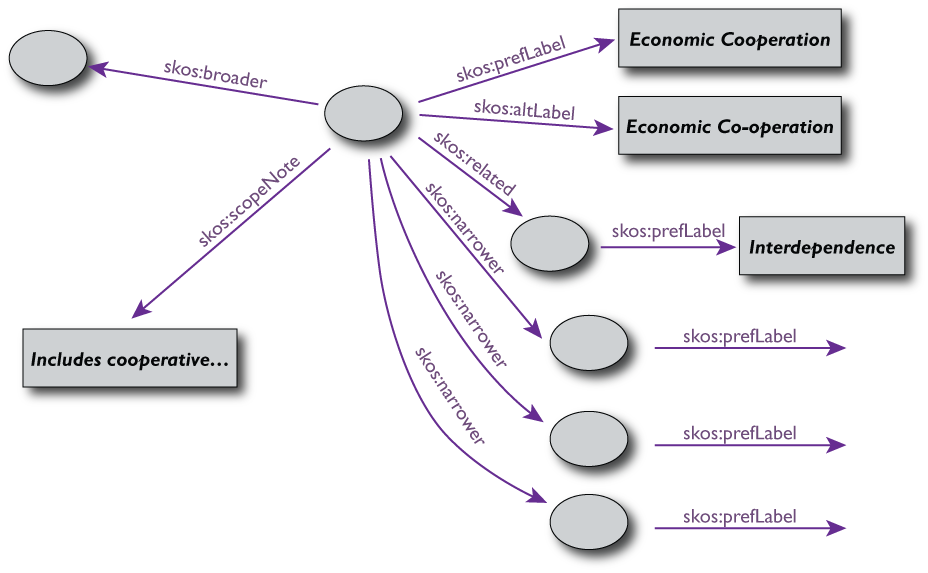
\includegraphics[width=13cm]{images/SKOS_simpleThesaurus.png}
	\caption[Modélisation simplifiée de \ac{skos}]{Modélisation simplifiée de \ac{skos} [Source: \href{https://www.w3.org/Consortium/Offices/Presentations/RDFTutorial/figures/SKOS_simpleThesaurus.png}{www.w3.org}]}
	\label{skos_modelisation}
\end{figure}
\medskip

Enfin, des propriétés de \ac{skos} permettent de créer du lien entre des concepts provenant de différentes sources: ce sont les propriétés d'équivalence ou de similitude <skos:broader>, <skos:exactMatch> ou <skos:closeMatch>. Ces propriétés permettent le rapprochement de plusieurs concepts: le \ac{lcsh}\footnote{Voir \reference{lcsh_liens}.} peut ainsi utiliser \ac{skos} pour créer des fiches de liens. De même, la Bibliothèque nationale de France (BnF) contient des références à l'ontologie Dewey qui lui permet ainsi d'obtenir des relations d'équivalence avec ses données. Alors, l'emploi de \ac{skos} nécessite des URIs de manière à créer des triplets \ac{rdf}.\\

Avec \ac{skos}, l'interopérabilité sémantique est désormais possible entre les institutions sur le Web de données. Cette ontologie \ac{rdf} permet de rapprocher des jeux de données et des référentiels jusqu'alors séparés et pourtant similaires. Le vocabulaire offert pour décrire les \textit{thesauri} et ensuite les partager dans le Web sémantique permet de nombreuses applications en institutions, et facilite ainsi les opérations d'indexation ou de recherche.

%conclu
\bigskip
\bigskip
Cependant, les vocabulaires des institutions n'étant pas nativement liés entre eux, il reste difficile de les aligner, et par conséquent de passer d'un \ac{kos} à une modélisation \ac{skos}, notamment pour les relations partie--tout. \nP{Sylvie}{Dalbin} prend en exemple\footcite{dalbin_approches_2011} ce type de relation qui peut être exprimé dans le Web sémantique par trois types de relations: hiérarchique, instance--classe, ou bien sous-classe--classe. Ces incertitudes rendent le processus d'ontologisation complexe, qui l'est d'autant plus quand les termes sont dans des langues différentes.\\

Les ontologies apparaissent comme un référentiel essentiel dans le Web de données, plus encore que les autorités qui sont devenues des données; elles ont permis l'apparition d'un Web sémantique. Seulement, la problématique de l'alignement de référentiels entre eux sur le Web de données est toujours présente et ne sera jamais totalement résolue.
\section{\label{II-B-3}Les ontologies dans le Web sémantique}
\titreEntete{Les ontologies dans le Web sémantique}

%intro
La finalité principale des ontologies est leur exposition sur le Web de données. L'utilisation qui s'ensuit permet la création d'un Web sémantique, structuré et aux données partagées. Le référentiel compris dans le sens de \ac{kos} n'intervient plus autant dans ce Web sémantique; le modèle de description de ces référentiels s'impose sous la forme des ontologies et améliore dans le même temps la description des concepts qu'il contient par des relations typées.\\

Cette avancée permet une description plus fine et partagée des documents des institutions patrimoniales: le référentiel est à la fois leur propres données et celles du Web de données, liées par les ontologies publiques.

\subsection{\label{II-B-3-a}Décrire des ontologies en \ac{rdf}: \ac{rdfs} et \ac{owl}}
\titreEntete{Décrire des ontologies en RDF}

De même que \ac{skos} est une ontologie permettant la description de \ac{kos}, \ac{rdfs} et \ac{owl} sont les représentations des ontologies \ac{rdf}. Les documents décrits par les institutions le sont par des formats et des logiques différentes. Utiliser une seule ontologie peut s'avérer difficile; en effet, elle peut être trop large ou trop spécifique pour le domaine décrit. C'est pourquoi l'utilisation des URIs, des liens hypertexte du Web, permet d'utiliser autant d'ontologies que nécessaire, et de créer une interopérabilité par parcours de liens, par rebonds sur les URIs.\\

La constitution de ce réseau de liens utilisé pour la description de documents n'est possible qu'avec l'utilisation du Web sémantique et de \ac{rdf}. C'est pourquoi il a été nécessaire de construire des modèles de représentation des ontologies en \ac{rdf}.\\

\ac{rdfs} est un langage de description simple, destiné à apporter les bases d'une description en \ac{rdf} avec la déclaration de classes --- et de sous-classes --- et de propriétés. Les classes sont des concepts, des types de ressources, identifiés par des URIs. Les propriétés sont les relations qui existent entre les classes. Ainsi, chaque ressource est instanciée à une classe par la propriété --- le prédicat \ac{rdf} --- <http://www.w3.org/1999/02/22-rdf-syntax-ns\#type> (rdf:type). La présence de sous-classes permet de créer des groupes au sein de classes: en déclarant une instance d'une sous-classe, un second triplet est alors implicitement créé entre la sous-classe et la classe avec le prédicat rdfs:subClassOf. Tout ce qui s'applique à une classe est appliqué à une sous-classe.\\

\ac{rdfs} admet aussi la déclaration de domaines et de codomaines pour les propriétés. Ces propriétés peuvent être de type ressource quand elles relient deux ressources désignées par des URIs, ou bien de type donnée quand l'objet est un littéral. Ce comportement des propriétés est déclaré avec le domaine et le codomaine: le domaine de la propriété définit la type de la classe sujet, tandis que le codomaine définit la classe de la ressource objet --- ou du type de donnée si c'est un littéral.\\

Malgré les classes et sous-classes, et les domaines et codomaines, \ac{rdfs} reste simple et ne permet pas de description complexe de relations. C'est pourquoi \ac{owl} est une extension de \ac{rdfs}. Des contraintes sur les relations comme la symétrie, l'équivalence, la différence ou la contradiction peuvent être exprimées; de même, la déclaration d'une liste d'instances contrôlées peut être faite. Comme avec \ac{skos}, il est possible, et souvent indispensable, de déclarer des relations d'équivalences entre les classes, les propriétés ou les instances. Ainsi, une instance peut hériter des propriétés de la classe à laquelle sa classe est équivalente. Pour cela, trois propriétés \ac{owl} existent: <http://www.w3.org/2002/07/owl\#equivalentClass> (owl:equivalentClass), <http://www.w3.org/2002/07/owl\#equivalentProperty> (owl:equivalentProperty) et <http://www.w3.org/2002/07/owl\#sameAs> (owl:sameAs).

\subsection{\label{II-B-3-b}Utilisation des ontologies en institutions}
\titreEntete{Utilisation des ontologies en institutions}

Chaque ontologie traitant d'un domaine particulier de la connaissance ou du monde, elles sont très nombreuses. Dans sa constante réflexion sur la description, l'indexation et le partage de ses données, le milieu bibliothéconomique s'est emparé du Web de données pour faciliter ses missions et la recherche. Ainsi, plusieurs ontologies sont essentielles dans ce milieu. La première, DC Terms\footcite{noauthor_dublin_nodate}, et la plus ancienne car créée en 1995, permet la description bibliographique d'un document sur le Web avec quinze propriétés, accompagnées de propriétés affinées --- \textit{abstract} l'est de \textit{description}. L'ontologie Dublin Core est constamment utilisée en bibliothèques\footnote{La \reference{onto_dcterms} montre la quantité d'ontologies l'utilisant.}, et plus généralement dans le Web de données, car elle offre les outils de base servant à la description d'un document.
\begin{figure}[!h]
	\centering
	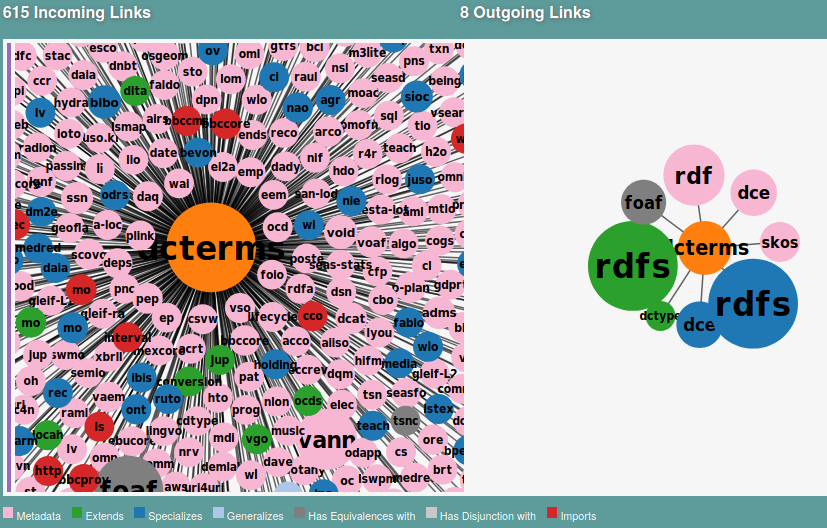
\includegraphics[width=13cm]{images/onto_dcterms.png}
	\caption[L'ontologie DC Terms]{DC Terms: représentation des ontologies l'utilisant (à gauche) et de celles qu'elle utilise(à droite) [Source: \url{https://lov.linkeddata.es/dataset/lov/vocabs/dcterms}]}
	\label{onto_dcterms}
\end{figure}
\medskip

Pour la description des autorités, l'ontologie \ac{foaf}\footcite{noauthor_foaf_nodate} est disponible et est également fortement utilisée. Créée au milieu des années 2000, elle permet la description des agents, de groupes et d'organisations, de personnes, mais aussi de réseaux sociaux.\\

Les ontologies propres aux institutions patrimoniales utilisent ces ontologies de haut niveau. Ainsi, \ac{bibo} utilise à la fois les DC Terms et \ac{foaf}. \ac{cidoccrm}\footnote{Voir \reference{annexe_onto} (\reference{onto_c4o})}, contrairement aux autres ontologies institutionnelles, n'est pas de bas niveau, mais de haut niveau. En effet, elle souhaite pouvoir décrire n'importe quel type d'objet: elle dispose de quatre-vingt-cinq classes et de plus de deux cent cinquante propriétés.

%conclu
\bigskip
\bigskip
\bigskip
Les \index[ref]{modelisation@Modélisation!frbr@FRBR}\index[ref]{relier@Relier!frbr@FRBR}\ac{frbr} et le modèle de données de la BnF permettent de conclure sur l'importance, pour les institutions, des ontologies dans le Web de données. En effet, son modèle de données étant basé sur les \ac{frbr}, tous les types de relations sont nécessaires pour relier l'œuvre aux points d'accès --- autorités, sujets, dates, \dots~ Ces relations sont exprimées par des ontologies publiques: l'exposition \index[ref]{echanges@Échanges!formats@Formats!rdf@RDF}\ac{rdf} des données permet alors l'utilisation des URIs des ontologies ainsi que la description fine du document décrit et de son contexte. Treize ontologies sont ainsi utilisées\footnote{Voir \reference{mdd_bnf}.}, uniquement partiellement pour les propriétés nécessaires à la BnF:
\begin{itemize}
	\item \index[ref]{relier@Relier!foaf@FOAF}\ac{foaf} pour les autorités;
	\item \index[ref]{echanges@Échanges!formats@Formats!rdf@RDF}\ac{rdf} pour exprimer les instances --- avec rdf:type ---;
	\item \index[ref]{relier@Relier!rdfs@RDFS}\ac{rdfs}
	\item \index[ref]{relier@Relier!skos@SKOS}\ac{skos} pour créer le concept préférentiel et définir les sujets proches 
	\item \index[ref]{relier@Relier!dcterms@DC Terms}DC Terms pour les descriptions bibliographiques simples
	\item Geo pour les descriptions géographiques
	\item \index[ref]{echanges@Échanges!formats@Formats!rda@RDA}\index[ref]{relier@Relier!rda@RDA}FRBR-RDA, RDAgroup2elements et RDArelationships pour exprimer les entités du modèle \ac{frbr}
	\item des ontologies internes, BNF-onto et BNFroles
	\item l'extension \ac{rdf} \index[ref]{relier@Relier!owl@OWL}\ac{owl}-time
	\item enfin une ontologie du langage de catalogage \ac{marc} MARCrel
\end{itemize}

L'exemple de la BnF montre qu'il n'y a plus de référentiel unique propre à une institution, mais seulement un ensemble de données dispersées dans le Web de données --- utilisation de \ac{rameau} notamment --- avec des ontologies qui permettent la production de sens sur les liens entre les ressources.\\

\begin{figure}[!h]
	\centering
	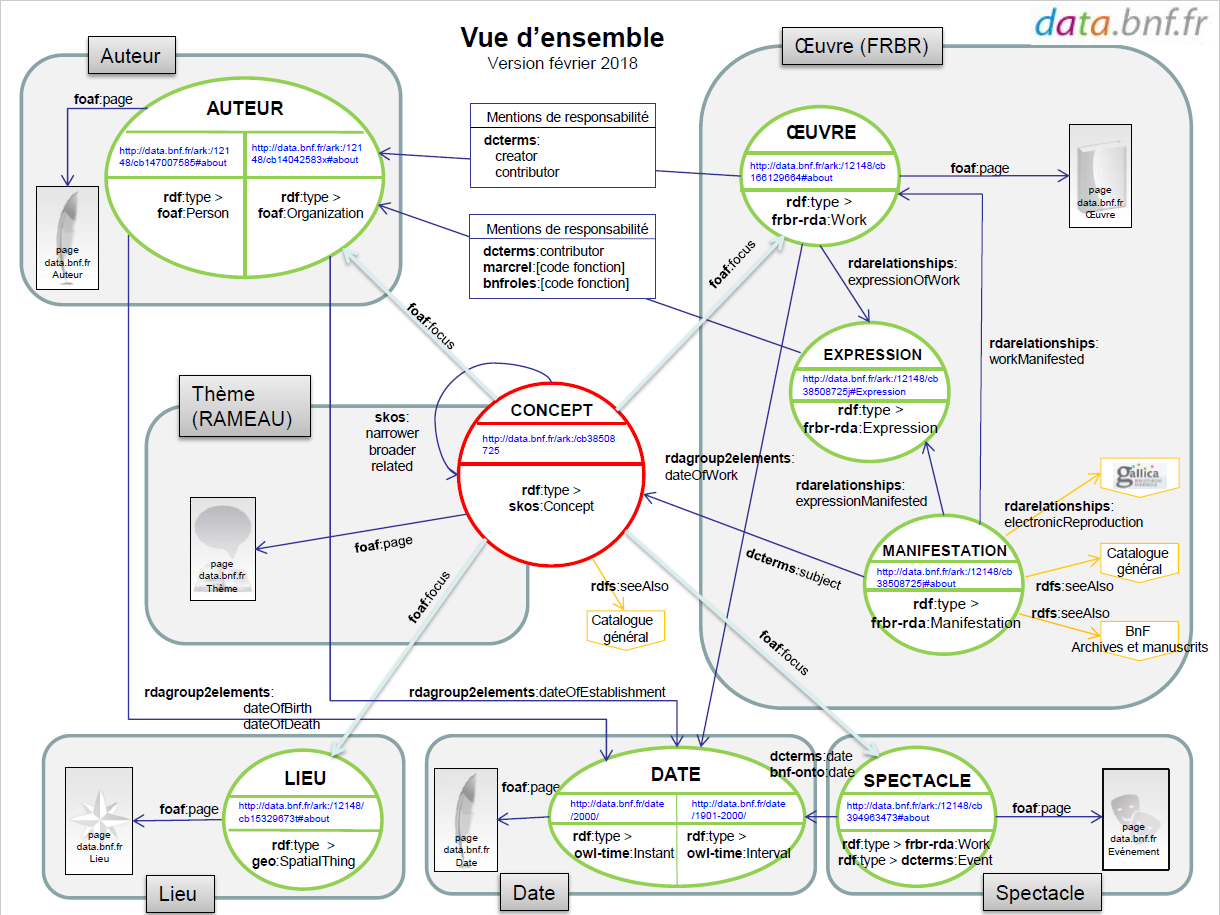
\includegraphics[width=15cm]{images/mdd_bnf.PNG}
	\caption[Le modèle de données de la BnF]{Le modèle de données de la BnF [Source: \url{https://data.bnf.fr/images/modele_donnees_2018_02.PNG}]}
	\label{mdd_bnf}
\end{figure}
	\chapter{\label{II-C}Relier ses données à Wikidata: l'exemple de l'alignement des personnes physiques de l'\ac{ina}}
\titreEntete{Relier ses données à Wikidata}

%intro
Si certaines institutions patrimoniales ont fait le choix d'exposer l'ensemble de leur données sur le Web avec le Web de données, certaines ne font pas ce choix. C'est le cas de l'\ac{ina}. En effet, l'Institut se concentre sur la mise en cohérence et la centralisation de ses données, tout en les enrichissant le plus possible. Dans ce but d'enrichissement des données, l'\ac{ina}, nous l'avons évoqué au \reference{I-B}, récupère des données complémentaires auprès de sociétés et créé ainsi du lien avec ces dernières par la conservation dans les bases de données des identifiants propres à chaque document et à chaque société. Cependant, les données fournies sont spécifiques à un domaine d'activité et restreintes. Par conséquent, l'utilisation du Web de données, avec des données ouvertes et accessibles à tous, permet la liaison avec plusieurs jeux de données et la récupération des informations manquantes.\\

\href{https://www.wikidata.org/}{Wikidata} est une base de connaissances collaborative \ac{rdf} concentrant le plus de données et de connaissances sur le monde. L'\ac{ina} utilise ainsi les identifiants de cette base comme liens vers les données qui y sont stockées\footnote{Le \reference{III-A} évoque en détail les possibilités offertes par Wikidata dans le parcours des liens et du graphe.}. Ces identifiants peuvent être ajoutés dès l'opération de catalogage des documents audiovisuels; ou bien ajoutés \textit{a posteriori} par un alignement.\\

Pour réaliser cet alignement entre des données institutionnelles et un jeu de données externes du Web sémantique, plusieurs outils existent:
\begin{itemize}
	\item Des logiciels comme \href{https://openrefine.org/}{Open Refine}\footnote{Ce logiciel est notamment utilisé par les archives Nationales pour aligner les personnes de la \href{http://www2.culture.gouv.fr/documentation/leonore/}{base Léonore de la Légion d'Honneur} avec Wikidata.} permettent d'aligner des données avec Wikidata en un clic sur l'interface; seulement, ce type de logiciel est peu personnalisable dans la constitution des requêtes effectuées.
	\item Des logiciels ETL permettant de créer des chaînes de récupération et de traitement des données, peu importe le lieu et le type de leur stockage. \href{https://www.talend.com/fr/}{Talend} est ainsi utilisé par l'\ac{ina}.
\end{itemize}
\medskip

De même que l'alignement entre les personnes physiques et le thésaurus de noms communs de l'\ac{ina}\footnote{Voir \reference{I-B}.}, celui-ci présente de nombreuses difficultés liées au langage naturel de chaque jeu de données. Plusieurs points de comparaison doivent alors être utilisés, ce qui multiplie les alignements avec Wikidata. De plus, ce type d'alignement révèle de multiples limites, tant techniques que linguistiques.

%input

%conclu
	
	%conclu
	%schéma global de la place du référentiel
	\newpage
	Cette seconde partie a mis en évidence une importante évolution dans la place des référentiels et les usages qui en sont faits. Ils ne se trouvent plus en marge des systèmes documentaires: les efforts donnés à les partager pour les réutiliser montre un glissement vers le centre de ces systèmes, sans toutefois l'atteindre. Le lien, plus que la donnée elle-même, est devenu un enjeu pour toutes les institutions: un enrichissement de ses propres données est possible. Ces partages constants ont montré l'importance des formats et des protocoles d'échanges communs et utilisés par tous.\\
	
	Deux cas de figure généraux de la place des référentiels dans les institutions et des liens qu'ils entretiennent entre eux sont apparus: d'une part il peut y avoir une simple réutilisation des données d'une institution dans une autre (\reference{schema_general_relier1}); d'autre part, le Web sémantique a permis la création de nouveaux référentiels avec lesquels il est possible de créer du lien (\reference{schema_general_relier2}).\\
	\begin{figure}[!h]
	\centering
	
	\begin{pspicture}(0,0)(14,7)
		\uput[0](0.8,6.4){Entrepôt de documents A}
		\uput[0](7.8,6.4){Entrepôt de documents B}
		%cercles globaux
		\pscircle(3,3){3}
		\pscircle(10,3){3}
		%cercles du A
		\pscircle(4.8,3.4){0.6}
		\pscircle(3,4.2){0.6}
		\pscircle(1.5,3.2){0.6}
		\pscircle(2.2,1.6){0.6}
		\pscircle(3.8,1.4){0.6}
		%cercles du B
		\pscircle(11.4,3.8){0.6}
		\pscircle(9.2,1.6){0.6}
		%labels du A
		\uput[0](2.6,4.2){D1}
		\uput[0](3.4,1.4){D2}
		\uput[0](1,3.2){D3}
		\uput[0](4.4,3.4){R1}
		\uput[0](1.7,1.6){R2}
		%labels du B
		\uput[0](8.8,1.6){D1}
		\uput[0](10.9,3.8){D2}
		%lignes du A
		\psline(4,2)(4.6,2.8)
		\psline(4.2,3.8)(3.6,4)
		\psline(3,3.6)(2.4,2.1)
		\psline(1.6,2.6)(1.85,2.25)
		%lignes du B
		\psline(8.8,2.1)(5.2,3)
		\psline(10.8,3.8)(5.4,3.4)
	\end{pspicture}
	
	\caption[Réutilisation d'un référentiel entre deux institutions]{Réutilisation d'un référentiel entre deux institutions (R: Référentiel; D: Document)}
	\label{schema_general_relier1}
\end{figure}
	%schémas
	
	Cependant, l'unique utilisation d'un seul référentiel ne permet pas à une institution de combler l'ensemble de ses besoins et de ses usages: plusieurs liens doivent alors être établis avec divers jeux de données, ce qui peut être réalisé par les ontologies et le passage de lien en lien. Bien que le lien soit devenu un élément structurant du Web sémantique, il devient d'autant plus précieux quand il se trouve lui-même objet d'une grande entité\footnote{Comme il a été montré sans autre précision avec \ac{viaf} dans le \reference{II-A}, et ce qui fera la suite de notre propos en \reference{centraliser}.}.
	\begin{figure}[h!]
	\centering
	
	\begin{pspicture}(0,0)(15.2,7)
		\uput[0](0.8,6.4){Entrepôt de documents A}
		\uput[0](9.8,6.4){Entrepôt de documents B}
		%cercles globaux
		\pscircle(3,3){3}
		\pscircle(12,3){3}
		%cercles du A
		\pscircle(3,4.6){0.6}
		\pscircle(1.5,3.6){0.6}
		\pscircle(2.2,1.6){0.6}
		\pscircle(4.2,3.1){0.6}
		%cercles du B
		\pscircle(13.4,3.8){0.6}
		\pscircle(11.2,1.6){0.6}
		%labels du A
		\uput[0](2.6,4.6){D1}
		\uput[0](3.8,3){D2}
		\uput[0](1,3.6){R2}
		\uput[0](1.7,1.6){D3}
		%labels du B
		\uput[0](10.8,1.6){D1}
		\uput[0](12.9,3.9){D2}
		
		%lignes du A
		\psline(1.9,4.1)(2.4,4.4)
		\psline(1.5,3)(1.95,2.1)
		\psline(2.8,1.6)(6.95,2.75)
		\psline(6.9,3)(4.8,3.1)
		\psline(3.6,4.7)(6.95,3.3)
		%lignes du B
		\psline(10.7,2)(8.05,2.7)
		\psline(12.8,3.8)(8.05,3.2)
		
		%ref web sem
		\pscircle(7.5,3){0.6}
		\uput[0](7.1,3){R}
	\end{pspicture}
	
	\caption[Utilisation commune d'un jeu de données du Web de données]{Utilisation commune d'un jeu de données du Web de données (R: Référentiel; D: Document)}
	\label{schema_general_relier2}
\end{figure}
	
	\part{\label{centraliser}CENTRALISER. Le référentiel, clé de voûte et pivot (depuis le milieu des années 2010)}	
	
	%intro
	
	\chapter{\label{III-A}Les labyrinthes comme réseaux de données et de liens}
\titreEntete{Les labyrinthes comme réseaux de données et de liens}

%intro
\lettrine{L}a multiplication des liens et de ceux possibles dans le Web de données entraîne, pour un humain, une désorganisation des informations et des référentiels dans ce Web de données. Les chemins à emprunter deviennent multiples et provoquent une ivresse de rebonds et d'informations chez l'utilisateur. Les interfaces de visualisation structurent l'ensemble des informations et des liens du Web de données, qui est devenu un Web où seule une machine peut se repérer rapidement et naviguer aisément. À partir du modèle du graphe d'un jeu de données, le Web de données a permis de créer un graphe à l'échelle du Web, accessible à tous et en tous points, depuis n'importe lequel des jeux de données, des référentiels ou des institutions.\\

La notion de graphe, de réseau de données, découle des nombreuses théories d'arbres de classifications et de descriptions des précédents millénaires. La constatation des limites et de l'échec de ces arbres a conduit à la théorisation, puis l'adoption dans le Web de données et par le milieu bibliothéconomique d'abord, du labyrinthe et du modèle-réseau de données. Le lien devenant l'essence-même de ces réseaux de données, de nouveaux types de référentiels ont vu le jour, notamment les \textit{hubs} de liens qui centralisent les liens et quelques données d'autorités autour d'un même identifiant. Wikidata, d'abord réceptacle structuré des données et des informations des Wikipédias, devient rapidement le hub de liens et d'identifiants le plus utilisé.

\section{\label{III-A-1}Du modèle encyclopédique aux graphes de données}
\titreEntete{Du modèle encyclopédique aux graphes de données}

%intro
Au Moyen-Âge, la dogmatique de l'arbre porphyrien domine. Ce n'est qu'à la Renaissance que le savoir est conçu comme ouvert. L'arbre était pensé selon le monde, pensé lui-même comme un cosmos clos et ordonné; ce même arbre était par ailleurs pensé comme une finitude inaltérable de sphères. Cependant, la pensée de Copernic influe la façon de concevoir le savoir: ce dernier s'efforce de mimer le système planétaire avec ses perspectives variables, des orbites qui deviennent des ellipses, \dots~\\

L'encyclopédie n'est alors plus qu'un amas de connaissances réelles et légendaires; elle devient un index devant décrire le monde et les connaissances, le classifier. La tension pesant sur ce modèle encyclopédique et la quantité infinie de connaissances conduisent à son éclatement au profit d'une forêt où tout est ou peut être relié selon les choix du lecteur.

\subsection{\label{III-A-1-a}Vers les labyrinthes (Renaissance)}
\titreEntete{Vers les labyrinthes}

L'évolution majeure de la Renaissance, faisant suite aux arbres porphyriens puis lulliens, est la nouvelle conception de la structure des éléments du monde: avec Porphyre et ses successeurs, seuls les accidents et les substances sont classifiés; avec la Renaissance, de multiples \index[ref]{typologie@Typologie!index@Index}index d'encyclopédies naissent, accompagnés de réflexions sur les manières d'ordonner le savoir\footnote{\og Nous n'avons plus affaire à une classification de substances et d'accidents, mais à l'index d'une encyclopédie possible et à la tentative de proposer un ordonnancement du savoir\fg{} in \cite{eco_arbre_2010}}. Toute la Renaissance va se concentrer sur cette classification du savoir.\\

La première grande encyclopédie tentant cette classification du savoir est l'\textit{Encyclopaedia septem tomis distincta} de \nP{Johann}{Alsted} en 1620\footcite{alsted_encyclopaedia_1630}: l'index devient la substance-même de cette œuvre. Cette encyclopédie s'inscrit dans la période pansophique de la Renaissance, dans laquelle la réflexion sur une sapience universelle, qui aurait toute l'étendue du savoir, est vive. Si l'arbre de Porphyre voulait simplement être un dictionnaire, un moyen de définir la science, l'index pansophique inspire quant à lui à classifier cette science, et s'éloigne donc du dictionnaire. Cette période pansophique marque bien l'arrêt de la conception hiérarchique du savoir, conçue comme moyen de définir: un autre moyen de décrire ce savoir est possible, en étant plus efficace.\\

Ce nouveau moyen part de la constatation que de multiples chemins peuvent mener à un même savoir. \nP{Francis}{Bacon} le constate, dès 1620, dans l'\textit{Instauratio Magna}\footcite{bacon_instauratio_1620} puis en 1626 dans le \textit{Sylva sylvarum}. Il n'est alors plus question d'arbre unique, mais d'arbres multiples, de labyrinthes avec des chemins ambigus, des ressemblances trompeuses, des spirales et des noeuds complexes\footnote{\og \textit{obliquae et implexae naturarum spirae et nodi}\fg{} in \cite{bacon_instauratio_1620}}. La forêt est un amas de sujets, on n'y trouve plus mais on découvre de nouvelles relations, ce que l'on ne connaissait pas encore et ce que l'on ne cherchait pas. Cependant, la \og tension entre l'arbre et le labyrinthe\fg{}\footcite{eco_arbre_2010} ne faiblit pas: \nP{John}{Wilkins}, à la fin des années 1660, est mis en échec devant ses classifications du savoir qui ne parviennent pas à classer les sujets; une table immense d'index est alors créée pour résoudre cette difficulté.\\

La masse des connaissances à classer étant immense, l'encyclopédie devient un inventaire général des connaissances, incapable de toutes les saisir: \nP{Gottfried Wilhelm}{Leibniz} comprend bien que l'entreprise encyclopédique peut être infinie en raison du nombre de renvois à créer pour s'adapter aux perspectives infinies d'accès à une connaissance. Le labyrinthe prend alors tout son sens: une connaissance est accessible par de multiples points d'accès et ne fait pas partie d'une hiérarchie stricte. Dans le \og Discours préliminaire\fg{} de l'Encyclopédie\footcite{diderot_encyclope_1751}, l'arbre porphyrien et la pensée artistotélicienne sont totalement remis en question. 
\begin{citationLongue}
	Le système général des sciences et des arts est une espèce de labyrinthe, de chemin tortueux, où l'esprit s'engage sans trop connaître la route qu'il doit tenir.\footcite[Discours préliminaire]{diderot_encyclope_1751}
\end{citationLongue}
L'encyclopédie totale et universelle ne pourra jamais voir le jour en raison de son ampleur; elle n'est qu'utopie de la connaissance. Cette utopie, toujours visible aujourd'hui --- les projets \index[ref]{lod@Linked Open Data (LOD)!wikidata@Wikidata}Wikidata ou Wikipédia se veulent le reflet de notre monde ---, ne cessera pas en raison du caractère culturel qu'elle contient: plus que le reflet de notre monde, elle est le reflet de notre culture et de nos cultures spécifiques. L'encyclopédie sert cependant à créer des portions d'encyclopédie, en vue de réaliser des classifications spécifiques à un domaine.

\subsection{\label{III-A-1-b}Des labyrinthes aux graphes}
\titreEntete{Des labyrinthes aux graphes}

L'arrivée de la pensée classificatoire au niveau du labyrinthe a eu lieu à plusieurs reprises, à chaque échec du modèle de l'arbre, notamment avec Porphyre où chaque pas dans l'arbre régénérait sans cesse l'arbre des différences: il n'y a, par conséquent, pas un, mais un nombre infini d'arbres selon leurs contextes. Il existe plusieurs types de labyrinthes dont les trois principaux sont présentés par \nP{Umberto}{Eco}:
\begin{itemize}
	\item Le plus ancien est un labyrinthe classique unicursal, dit de Knossos (\reference{annexe_laby} (\reference{laby_knossos})): la seule possibilité est d'atteindre son centre; en raison de cette caractéristique, il ne peut pas se rapporter à un modèle encyclopédique, ni à un modèle de description des connaissances. En effet, le savoir n'est pas un long couloir dans lequel on accède toujours à la même connaissance.
	\item Le labyrinthe maniériste d'Irrweg permet des choix alternatifs (\reference{annexe_laby} (\reference{laby_irrweg})): toutes les routes mènent à des points morts, sauf un qui est la sortie. Ce labyrinthe est un arbre de décisions, dans lequel les branches sont la représentation des décisions possibles.
	\item Enfin, le labyrinthe qui donne naissance aux réseaux et aux \index[ref]{typologie@Typologie!graphe@Graphe de nœuds et de liens}graphes est le \og labyrinthe réseau\fg{} de \nP{Umberto}{Eco} (\reference{annexe_laby} (\reference{laby_reseau})). Chaque point du labyrinthe peut être connecté à n'importe quel autre point. Cette structure a l'avantage d'être extensible à l'infini, il permet des connexions infinies et des corrections locales qui ne modifient pas le reste du labyrinthe. Évolutif, ce labyrinthe nécessite de l'utilisateur qu'il modifie en permanence l'image qu'il s'en fait: \og Un réseau est un arbre auquel il faut ajouter des couloirs infinis connectant ses noeuds\fg{}\footcite{eco_arbre_2010}.
\end{itemize}
\medskip
Modèle dans lequel les connexions, les liens, sont essentiels, le labyrinthe réseau permet une représentation multidimensionnelle des connaissances et un accès à un point précis par de multiples liens. En 1968, \nP{Ross}{Quillian}\footcite[p.227-270]{minsky_semantic_1968} fait apparaître le réseau sémantique structuré, conçu comme un réseau de nœuds interconnectés\footnote{\og \textit{The memory model consists basically of a mass of nodes interconnected by different kinds of associative links}\fg{} in \cite[p.234]{minsky_semantic_1968}}. Le modèle qu'il décrit part d'un terme souche qui est défini par une série de nœuds, des tokens: ce n'est pour l'instant qu'un arbre. Seulement, les tokens peuvent à leur tour devenir des souches et porter des relations d'association: le réseau est ainsi constamment remodelé et modifié\footnote{\og \textit{Token nodes make it possible for a word's meaning to be built up from other word meanings as ingredients and at the same time to modify and recombine these ingredients into a new configuration}\fg{} in \cite[p.234]{minsky_semantic_1968}}. Ce modèle en réseau permet alors la définition de chaque terme, par ses connexions, avec tous les autres termes; il devient infini et multidimensionnel, non représentable en entier sur un plan bidimensionnel: la complexité du modèle-réseau peut être uniquement traité et compris par une machine. 

%conclu
\bigskip
\bigskip
L'apparition du modèle-réseau, du labyrinthe-réseau, a montré l'importance du lien dès la seconde moitié du \textsc{XX}\textsuperscript{ème}siècle. L'informatique a permis de mettre fin aux structures de connaissances qui étaient concevables par un esprit humain, afin de laisser la machine représenter les données dans toute leur complexité. Ce modèle, beaucoup plus efficace et riche que les arbres, consacre la valeur du lien, qui devient lui-même plus important que la donnée: il définit et légitime la donnée.
\section{\label{III-A-2}Des labyrinthes d'identifiants: les hubs de liens}
\titreEntete{Les hubs de liens}

%intro
La modélisation des données sous la forme de labyrinthes --- ou de graphes --- a un impact  considérable dans le Web de données: certains jeux de données sont eux-mêmes stockés dans une base de données graphe --- comme Wikidata qui fonctionne sur la base de données Blazegraph---; ou alors les jeux de données peuvent entre eux former un gigantesque graphe, infini. Cette seconde conception du modèle-réseau de \nP{Umberto}{Eco} est au centre du Web de données. Avec la décentralisation des référentiels sur le Web et leur éclatement en de multiples données, il est apparu comme nécessaire de les recentraliser au travers de nouveaux référentiels fournisseurs d'un unique identifiant.\\

Cependant, la recentralisation passe également par l'ajout de données, parallèlement à l'ajout des liens. En effet, nous l'avons montré au \reference{II-C}: les données peuvent varier dans leur graphie et leur forme selon le référentiel duquel elles sont issues. Afin d'offrir des données utilisables par tous, certaines plateformes ajoutent, pour chacun de leurs identifiants, des données préférentielles aux côtés des liens pointant vers d'autres référentiels ou jeux de données.

\subsection{\label{III-A-2-a}De la décentralisation des référentiels à leur recentralisation dans le Web de données}
\titreEntete{De la décentralisation des référentiels à leur recentralisation}

La multiplication du nombre de référentiels dans le Web de données conduit à une profusion de données et à leur répétition, sans que soient repérées les données se rapportant à un même concept\footnote{La constellation du Linked Open Data montre cette augmentation croissante du nombre de référentiels dans le Web de données, et l'absence, pour certains, de liens vers d'autres référentiels. Voir \reference{annexe_lod} (\reference{lod_cloud}).}. L'importance prise par ces référentiels partagés, mis en commun, et réutilisés par tous, a provoqué une recentralisation autour de nouveaux référentiels, nés de l'agrégation d'autres de ces référentiels.\\

Étonnante au premier abord puisqu'elle reconstruit des jeux de données alors que le mouvement inverse a été initié avec le Web de données pour plus d'efficacité, cette réaction s'explique par la nécessité de créer davantage de liens entre les données et les référentiels\footnote{\og Ironie de l’histoire, alors que le Linked Open Data souhaitait mettre en relation des données hétérogènes et décentralisées chez différents fournisseurs, il aura suffi de 5 ans pour que les utilisateurs commencent à recentraliser leurs données au sein d’un espace unique\fg{} in \cite{poupeau_au-a_2018}}. Ces nouveaux référentiels constituent alors des \og hubs\fg{} centralisant et exposant les données et les liens selon les règles et les principes du Web de données. \index[ref]{lod@Linked Open Data (LOD)!wikidata@Wikidata}Wikidata a ici un rôle majeur et prouve qu'une base de connaissances unique et centralisée est essentielle.\\

Si Wikidata est une base ouverte, des enjeux commerciaux peuvent également s'emparer de cette problématique de la structure des données sur le Web et de la description des documents nativement numériques: Google créé ainsi une base de connaissances parallèle --- le Knowledge Graph ---, elle aussi sous la forme d'un graphe mais n'utilisant pas \ac{rdf}, utilisant Wikidata comme une source de données. De même qu'un langage universel était nécessaire pour décrire les documents sur le Web, un langage est nécessaire pour décrire les sites Web et leur offrir en échange un meilleur référencement: la puissance de Google, associé à Yahoo et Microsoft, lui permet ainsi d'imposer l'ontologie \index[ref]{relier@Relier!schema@schema.org}\href{https://www.schema.org}{schema.org} comme standard du Web pour la description des sites\footcite{poupeau_au-a_2018}, rejetant \index[ref]{echanges@Échanges!formats@Formats!rdf@RDF}\ac{rdf}a au profit de \ac{json}-LD\footnote{Une sérialisation en \ac{json} adaptée aux données liées. Voir \url{https://www.w3.org/TR/json-ld/}.}.\\

Le Knowledge Graph et l'ontologie schema.org sont les meilleurs exemples de l'utilisation idéale du Web de données et du Web sémantique. Ils ont été créés spécialement pour centraliser les données et y accéder par le seul langage machine. \index[ref]{lod@Linked Open Data (LOD)!wikidata@Wikidata}Wikidata, qui apparaît comme le référentiel le plus élevé dans le milieu bibliothéconomique\footnote{Voir \reference{III-A-2-c}.}, n'est plus qu'une source de données structurées pour les robots des moteurs de recherche utilisant \index[ref]{relier@Relier!schema@schema.org}schema.org. Le référentiel a désormais acquis la place principale, centrale, dans l'administration de données et leur recherche.

\subsection{\label{III-A-2-b}Apparition des hubs de liens et d'identifiants}
\titreEntete{Apparition des hubs de liens et d'identifiants}

De même que les ontologies apportent une couche supplémentaire aux données, en les liant entre elles malgré leurs différences, des hubs se forment pour centraliser les identifiants de différents référentiels afin d'avoir un unique lieu où y seront puisés d'autres identifiants: c'est le principe de l'interopérabilité par suivi de liens. Ces nouveaux hubs se trouvant dans le Web de données, il est normal et indispensable qu'ils se créent sur les principes et les formats qui le composent. Ainsi, ces hubs forment des concepts, ou des entités, qui rassemblent les liens de vedettes et de concepts identiques. Ces nouveaux concepts sont également désignés par des URIs servant d'identifiant pour chacun d'eux.\\

Ces hubs prennent une place centrale dans le Web de données et deviennent indispensables. Seulement, il peut être risqué de ne conserver, dans un système documentaire, qu'un seul identifiant, celui de ce hub. En effet, aucun de ces identifiants ou de ces liens --- y compris les identifiants ark: de la Bibliothèque nationale de France (BnF) --- ne peuvent être considérés comme pérennes et sûrs. Au-delà des identifiants qui disparaissent sur le Web, les données qui leur sont associées sont supprimées\footnote{\og De très nombreuses initiatives d’exposition des données ont aujourd’hui disparu, emmenant avec elles non seulement les identifiants mais aussi les données elles-mêmes\fg{} in \cite{poupeau_au-a_2018}}. Certes, l'ampleur de Wikidata peut laisser penser que les entités et leurs identifiants seront disponibles à long terme, mais des aléas techniques, financiers ou politiques peuvent très bien conduire à la fermeture de ce service et donc à la disparition de l'ensemble des données. Nous verrons par la suite (\reference{III-A-3}) que la récupération de quelques identifiants majeurs est nécessaire en plus de l'identifiant de Wikidata, afin d'avoir à la fois un accès direct à ces identifiants --- sans suivre les liens --- et une relative sécurité quant à la conservation d'un lien avec un référentiel externe.\\

\begin{figure}[h!]
	\centering
	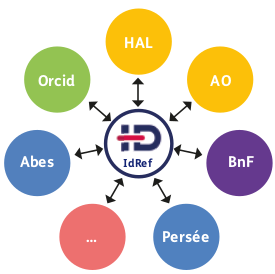
\includegraphics[width=7cm]{images/idref.png}
	\caption[La fédération entreprise par \ac{idref}]{La fédération entreprise par \ac{idref} [Source: \cite[p.9]{aymonin_arabesques_2017}]}
	\label{idref_schema}
\end{figure}

\index[ref]{lod@Linked Open Data (LOD)!viaf@VIAF}\index[ref]{autorites@Autorités!viaf@VIAF}\ac{viaf}, \index[ref]{lod@Linked Open Data (LOD)!idref@IDREF}\index[ref]{autorites@Autorités!idref@IDREF}\ac{idref} ou \index[ref]{lod@Linked Open Data (LOD)!lcsh@LCSH}\index[ref]{autorites@Autorités!lcsh@LCSH}\ac{lcsh} sont quelques uns de ces hubs de liens qui fournissent en une seule page plusieurs identifiants. \ac{idref} est basé sur les autorités du Sudoc, mais a été créé pour effectuer l'interopérabilité entre les différents catalogues du milieu de la recherche à travers un référentiel commun\footnote{\og Il s’agissait de montrer la fonction de pivot des identifiants et les bénéfices d’un adossement des catalogues à un référentiel commun.\fg{} in \cite[p.9]{aymonin_arabesques_2017}}. Ainsi, de multiples référentiels sont liés avec \ac{idref} par leur identifiant~(\reference{idref_schema}): \index[ref]{lod@Linked Open Data (LOD)!rameau@RAMEAU}\index[ref]{autorites@Autorités!rameau@RAMEAU}\ac{rameau} est utilisé, de même que HAL pour les publications scientifiques ouvertes ou Persée; les identifiants \ac{viaf} et \ac{isni} sont également renseignés, \dots


\subsection{\label{III-A-2-c}Les hubs de liens et d'identifiants réceptacles de données}
\titreEntete{Les hubs de liens et d'identifiants réceptacles de données}

\begin{citationLongue}
	D’un hub de références, Wikidata tend à devenir un réceptacle des données elles-mêmes\footcite{poupeau_au-a_2018}.
\end{citationLongue}
\medskip

Le projet \index[ref]{lod@Linked Open Data (LOD)!wikidata@Wikidata}Wikidata est né en 2012 de la volonté de centraliser les informations des Wikipédias sous la forme de données structurées en déclarations. Ce modèle de données ressemble à \index[ref]{echanges@Échanges!formats@Formats!rdf@RDF}\ac{rdf}, mais reste différent en raison des informations supplémentaires apportées par le modèle Wikidata: l'ajout de références et de qualificatifs enrichit les données. Wikidata s'impose dans le Web de données par ses atouts: ses données, augmentées par une communauté imposante, sont disponibles immédiatement et ne dépendent pas des mises à jour --- comme cela était le cas avec \index[ref]{lod@Linked Open Data (LOD)!dbpedia@DBpédia}DBpédia ---; les données de Wikidata se requêtent avec \index[ref]{echanges@Échanges!protocoles@Protocoles!sparql@SPARQL}\ac{sparql}.\\

Premièrement, Wikidata est un hub d'identifiants, de liens. Ces identifiants font l'objet, sur les pages d'entités de Wikidata, d'une partie à part, à la fin de cette page. Ils sont néanmoins de simples déclarations propriété--valeur avec une possibilité d'ajouter des qualificatifs et des références\footnote{Un compte Twitter, qui a un identifiant et qui peut par conséquent faire l'objet d'une déclaration dans une entité de Wikidata, a, par exemple, comme qualificatif le nombre d'abonnés à une date donnée.}.
L'ensemble --- plusieurs centaines --- des propriétés d'identifiants est répertorié sur la page de liste de ces propriétés \href{https://www.wikidata.org/wiki/Wikidata:List_of_properties/Wikidata_property_for_an_identifier}{Wikidata:List of properties/Wikidata property for an identifier}: les jeux de données et les référentiels étant de plus en plus nombreux sur le Web, ces propriétés permettent de typer et de décrire chaque relation avec un identifiant.\\

Deuxièmement, \index[ref]{lod@Linked Open Data (LOD)!wikidata@Wikidata}Wikidata est un réceptacle de données. En effet, en plus des identifiants, Wikidata propose des déclarations structurées biographiques ou générales sur l'entité. En cela, si \index[ref]{lod@Linked Open Data (LOD)!idref@IDREF}\index[ref]{autorites@Autorités!idref@IDREF}\ac{idref} et Wikidata semblaient être similaires avec l'offre de liens, ils diffèrent par cette structuration permanente des informations. Ainsi,  le concept \nP{Vincent}{Dedienne} de \ac{idref}\footnote{\nP{Vincent}{Dedienne} dans \ac{idref}: \url{https://www.idref.fr/196914183}\\\nP{Vincent}{Dedienne} dans Wikidata: \url{https://www.wikidata.org/wiki/Q18413745}} structure l'état civil et les dates, mais met le reste des informations en note: \og Comédien,auteur , acteur et humoriste français\fg{}. Wikidata apporte du sens grâce à la propriété P106 qui permet d'indiquer que la déclaration concerne l'\textit{occupation} de la personne, et d'offrir un lien vers l'entité de cette occupation.\\

Par la structuration de ses données et l'apport de multiples identifiants et liens vers d'autres jeux de données et référentiels, \index[ref]{lod@Linked Open Data (LOD)!wikidata@Wikidata}Wikidata devient un \textit{super} hub, se plaçant plus haut encore que ceux évoqués précédemment.

%conclu
\bigskip
\bigskip
L'agrégation de liens et d'identifiants est un enjeu essentiel de manière à n'effectuer des opérations d'alignement qu'une seule fois, et ainsi diminuer le coût de ces opérations. Ces agrégations nécessitant elles-mêmes des identifiants pour pouvoir exister sur le Web de données, des données structurées sont venues s'ajouter à la simple exposition de liens vers d'autres référentiels. Ainsi, Wikidata a montré son efficacité et se place aujourd'hui comme acteur principal d'agrégation de connaissances et de liens vers d'autres sources de données souvent plus spécialisées.
\section{\label{III-A-3}Wikidata comme hub de liens: aligner les fictions et les séries de l'INA avec Wikidata}
\titreEntete{Wikidata comme hub de liens}

%intro
Le principal intérêt de Wikidata, nous l'avons évoqué précédemment, est l'agrégation de liens et d'identifiants d'autres référentiels et jeux de données. Cela permet d'accéder à un même endroit à divers identifiants de référentiels, sans avoir à effectuer un alignement avec chacun de ces référentiels. L'opération d'alignement de fictions et de séries avec Wikidata ne peut s'effectuer qu'à partir des titres: alors qu'un alignement de personnes se réalise sur un voire deux mots de l'état civil, celui de titres et de séries doit se réaliser sur l'ensemble des mots de ces titres, ce qui augmente considérablement les échecs d'alignement.\\

Cependant, malgré les difficultés, imposées une nouvelle fois par le langage naturel, l'alignement reste une opération importante pour l'enrichissement des données d'une institution: le parcours de liens devient alors possible, et l'accès au Web de données apporte de nouvelles informations sur les instances alignées.

\subsection{\label{III-A-3-a}Enrichir ses données avec des identifiants plutôt qu'avec des textes}
\titreEntete{Enrichir ses données avec des identifiants}

L'établissement de liens avec des référentiels externes est essentiel à l'\ac{ina}. En effet, les données issues du \ac{dl} sont parfois sommaires et tournées vers l'événement de diffusion au détriment de la description documentaire. Si les données achetées à l'extérieur --- auprès de Plurimédia, Médiamétrie, \dots --- apportent les informations les plus importantes, l'ensemble des acteurs d'une série ou d'une fiction ne sont par exemple pas présents dans les bases de données de l'\ac{ina}.\\

Une première possibilité serait alors d'aligner les fictions et les séries avec Wikidata afin de récupérer les libellés des valeurs de la propriété P161 qui permet la déclaration de membres du casting. Cette possibilité nécessiterait néanmoins une mise à jour régulière avec un nouveau lancement de l'alignement, de manière à avoir les données et les informations actualisées de Wikidata. De plus, l'introduction de ces textes coupe les liens qui étaient présents sur Wikidata, et empêche ainsi de naviguer de lien en lien depuis un membre de casting, par exemple, pour arriver sur une autre de ses fictions.\\

Le stockage du seul identifiant de l'entité Wikidata de la fiction ou de la série suffit alors. À partir de cet identifiant, il devient possible d'accéder à toutes les déclarations de l'entité, qu'elles soient biographiques ou générales, ou bien qu'elles soient des liens, ainsi qu'aux déclarations des valeurs de ces déclarations, \dots~ L'alignement des fictions et des séries de l\ac{ina} vise apr conséquent à récupérer les identifiants Wikidata des fictions, des séries, et des épisodes de séries.\\

Parallèlement à cette récupération d'identifiants Wikidata, il est également nécessaire d'obtenir l'\ac{isan}, l'identifiant international de tout document audiovisuel. Cet \ac{isan} permet alors d'obtenir par rebond des informations plus précises sur la fiction ou la série grâce à une base de données spécifique, IMDb\footcite{noauthor_imdb_nodate}. Le stockage à l'\ac{ina} de simples identifiants --- Plurimédia, Médiamétrie, IMédia, Wikidata et \ac{isan} --- est alors suffisant pour avoir accès au Web de données et à l'ensemble des informations et des données disponibles sur ces instances.

\subsection{\label{III-A-3-b}Aligner des fictions et des séries avec Wikidata}
\titreEntete{Aligner des fictions et des séries avec Wikidata}

De même que l'alignement des personnes physiques avec Wikidata\footnote{Voir \reference{II-C}.}, le \ac{sparql}-EndPoint et l'\ac{api} Wikibase sont conjointement utilisés. Une première étape nécessite la récupération de l'ensemble des sous-classes des entités \textit{Film} (Q11424)\footnote{Film (Q11424): \url{https://www.wikidata.org/wiki/Q11424}} et \textit{Série Télévisée} (Q5398426)\footnote{Série Télévisée (Q5398426): \url{https://www.wikidata.org/wiki/Q5398426}} par une requête \ac{sparql} (\reference{sparql_1}).
\begin{figure}[!h]
	\centering
	\begin{minted}{sparql}
select ?serie ?serieLabel
where{
?serie wdt:P279* wd:Q5398426.
service wikibase:label{bd:serviceParam wikibase:language "fr,en"}
}
	\end{minted}
	\caption{Requête \ac{sparql} pour récupérer les sous-classes de l'entité \textit{Série Télévisée}}
	\label{sparql_1}
\end{figure}
Dans le cas des séries télévisées, d'autres entités, non présentes dans la requête de la \reference{sparql_1}, sont nécessaires pour avoir accès à l'ensemble des séries télévisées de Wikidata. Il est ainsi nécessaire de faire une seconde requête avec la propriété P361 qui indique qu'une entité est \og une partie d'\fg{}une autre entité: l'entité de la \textit{saison} (Q3464665)\footnote{Saison (Q3464665): \url{http://www.wikidata.org/entity/Q3464665}}, essentiel dans l'alignement, est récupéré par ce moyen.\\

La récupération des instances de chacune des sous-classes est ensuite possible par une requête \ac{sparql}\footnote{Le \ac{sparql}-EndPoint est ici utilisé en raison du faible nombre de requêtes qui seront effectuées, et du nombre de résultats par requête relativement faible (inférieur à 200000) n'induisant pas de \textit{timeout}.} (\reference{sparql_2}). L'objectif de cette étape n'est pas de récupérer l'ensemble des valeurs des propriétés qui permettent l'alignement --- ce qui ne serait pas possible en raison des limites du \ac{sparql}-EndPoint évoquées au \reference{II-C} ---, mais d'obtenir les identifiants de toutes les entités instances des sous-classes.
\begin{figure}[!h]
	\centering
	\begin{minted}{sparql}
select ?saison ?saisonLabel
where{
?saison wdt:P31 wd:Q3464665.
service wikibase:label{bd:serviceParam wikibase:language "fr,en"}
}
	\end{minted}
	\caption{Requête \ac{sparql} pour récupérer les identifiants des instances de la classe \textit{Saison}}
	\label{sparql_2}
\end{figure}

L'\ac{api} Wikibase, avec le module \textit{wbgetentities} permet ensuite d'obtenir les points de comparaison avec les données de l'\ac{ina}:
\begin{itemize}
	\item pour les fictions, les valeurs suivantes sont ainsi récupérées:
	\begin{itemize}
		\item P577 pour la date de publication de la fiction
		\item P57 pour le réalisateur
		\item P162 pour le producteur
		\item les libellés préférentiels et alternatifs du titre et des noms de personnes sont également ajoutés
	\end{itemize}
	\item pour les séries, plus précisément les épisodes, les suivantes:
	\begin{itemize}
		\item P577 pour la date de publication de l'épisode
		\item P179 pour la série d'appartenance de l'épisode
		\item le qualificatif P1545 de P179 pour le numéro de l'épisode
		\item P4908 pour le nom de la saison
		\item le qualificatif P1545 de P4908 pour le numéro de la saison
		\item les libellés préférentiels et alternatifs des titres sont récupérés en français et en anglais --- en effet, un grand nombre de séries conservées à l'\ac{ina} n'ont pas de titres traduits
		\item les libellés préférentiels et alternatifs des valeurs des propriétés sont récupérés uniquement en français
	\end{itemize}
\end{itemize}

Cette récupération de différentes données permet un alignement avec les données de l'\ac{ina}. La fiction long métrage \og Doux dur et dingue\fg{} de \nP{James}{Fargo} en 1978 trouve ainsi son entité équivalente (\href{https://www.wikidata.org/wiki/Q1195524}{Q1195524}) dans Wikidata grâce à une stricte égalité --- après passage des majuscules en minuscules et suppression de la ponctuation --- des titres: l'\ac{isan} (déclaré avec la propriété P3212) \og 0000-0000-3B9A-0000-D-0000-0000-Z\fg{} peut alors être ajouté aux données de l'\ac{ina} en plus de l'identifiant Wikidata.
Pour les séries, ce sont les épisodes qui subissent l'alignement car chacun d'entre eux est identifié individuellement et lié ensuite avec sa série d'appartenance: le troisième épisode de la comédie de situation \og 3ème planète après le Soleil\fg{}, \og The Fifth Solomon\fg{}, est alors aligné doublement. Il l'est une première fois avec sa série (\href{https://www.wikidata.org/wiki/Q870490}{Q870490}), et une seconde fois avec son entité équivalente dans Wikidata, \href{https://www.wikidata.org/wiki/Q18040623}{Q18040623}. Enfin, l'\ac{isan}, quand il est disponible, est également ajouté, ce qui est le cas pour cet épisode identifié internationalement par l'identifiant \og 0000-0001-637C-0065-4-0000-0000-P\fg{}.

\subsection{\label{III-A-3-c}Les difficultés posées par les langages naturels}
\titreEntete{Les difficultés posées par les langages naturels}

Les résultats obtenus après un alignement de fictions ou de séries avec Wikidata peuvent paraître faibles: si les fictions sont alignées presque à 50\%, ce n'est pas le cas des séries pour lesquelles à peine 10\% des épisodes ont pu être alignés avec leur équivalent Wikidata. Bien que de nombreux épisodes et séries n'existent pas sur Wikidata, comme \og Mon père dort au grenier\fg{} dont il existe 26 saisons, cette absence d'entités Wikidata n'est pas suffisante pour expliquer les faibles alignements des séries.\\

La raison principale est le langage naturel utilisé de chaque côté de l'alignement, et les nombreuses divergences de graphie qui peuvent exister sur les mots des titres. En effet, les titres des séries sont pour certains traduits en français, d'autres restent en anglais, à la fois dans les données de l'\ac{ina} et sur Wikidata. L'alignement n'utilisant pas de traducteur ou d'intelligence artificielle, la similarité entre, par exemple, l'instance de l'\ac{ina} \og Monk va à la noce\fg{} de la saison 7 de Monk, avec l'entité \href{https://www.wikidata.org/wiki/Q50846176}{Q50846176} \og Mr. Monk Goes to a Wedding\fg{} qui lui correspond. L'alignement n'aura alors réussi à aligner que la série d'appartenance (Q189068) de cet épisode, et non l'épisode lui-même. L'utilisation des libellés préférentiels et alternatifs en français et en anglais aura, ici, été inutile. Cependant, la prise en compte de l'anglais a permis de nombreux alignements d'épisodes qui, tant du côté de l'\ac{ina} que de Wikidata, n'ont pas été traduits.\\

De plus, des séries très longues, comme \og Amour, gloire et beauté\fg{}, qui compte plus de 5000 épisodes, peuvent ne pas être décrites dans Wikidata au niveau de l'épisode. Quand une entité d'épisode est disponible dans Wikidata et que ce titre ne correspond pas à celui de l'\ac{ina}, il est possible d'utiliser le numéro de saison et d'épisode pour effectuer l'alignement. Seulement, le comptage des épisodes est différent selon Wikidata et l'\ac{ina}: Wikidata ne réinitialise pas le numéro d'épisode au début de chaque saison, alors que l'\ac{ina} le fait le plus souvent.\\

Les difficultés à l'alignement des fictions et des séries sont multiples, ce qui entraîne un faible rendement, notamment quand il s'agit d'aligner à la fois un libellé et un autre libellé d'une valeur de déclaration. Les graphies et les langues varient énormément. Les limites d'un alignement par stricte égalité sur des textes sont certainement ici atteintes. Des méthodes alternatives seraient nécessaires comme l'utilisation d'un traducteur puis de réseaux de neurones permettant d'aligner sur des similarités de textes et des égalités de numéro de saison ou de producteur.

%conclu
\bigskip
\bigskip
Bien que nécessaire, la récupération d'identifiants et de liens sur le Web de données, principalement sur Wikidata, peut se révéler difficile selon le type de données permettant l'alignement, et le genre des entités et des instances. L'alignement de personnes, effectué sur peu de mots et des données structurées comme les dates, est ainsi plus facile à réaliser que l'alignement de séries qui ne peut se faire qu'à partir d'une longue chaîne de caractères, le titre.

%conclu
\bigskip
\bigskip
\bigskip
Le succès des modèles de données en graphe est incontestable et est repris dans tous les projets d'envergure internationale: nous avons déjà évoqué Wikidata, le projet European Holocaust Research Infrastructure (EHRI)\footnote{Site du projet: \cite{noauthor_european_nodate}\\Utilisation du graphe de données: \cite{blanke_developing_2015}} peut également être cité comme acteur institutionnel se dégageant des bases de données relationnelles et des traditionnels référentiels hiérarchiques et contrôlés. Cependant, ce modèle de graphe nécessite un langage de requête efficace et des rendements élevés. Or, il a été constaté, avec Wikidata et le \ac{sparql}-EndPoint, des lenteurs de retours de résultats, obligeant à utiliser d'autres moyens pour obtenir les entités de Wikidata avec leurs déclarations.\\

La recentralisation des données autour de quelques acteurs du Web de données est une conséquence inattendue de la décentralisation de ces mêmes données qui avait eu lieu quelques années auparavant, avec la publication de jeux de données et de référentiels sur le Web sémantique. Cette recentralisation est née d'un besoin d'obtenir en un même endroit une multiplicité de liens, d'identifiants et d'informations, sans avoir à connaître les institutions ou les jeux de données dans lesquels aller chercher les données nécessaires. Si cette recentralisation concerne ici le Web de données, elle peut également concerner les institutions directement, ainsi que les entreprises: on ne parle alors plus de Linked Open Data, mais de Linked Enterprise Data (LED).
	\chapter{\label{III-B}Le \ldd de l’\ac{ina} : le référentiel au centre du modèle}
\titreEntete{Le référentiel au centre du modèle}

%intro
L'impact du \ac{lod} sur la structure des données et l'éclatement des référentiels a été l'un des aspects de la refonte des systèmes d'information en institutions ou en entreprises, sous la forme de \ac{led}. Ces \ac{led} sont des modèles de données à la structure similaire au \ac{lod}, ce qui les rend très efficaces et utiles dans l'utilisation des données qui en découle.\\

Le \ldd de l'\ac{ina} est l'un de ces \ac{led}: il a vocation à regrouper l'ensemble des métadonnées de l'Institut, en provenance de plusieurs départements sous diverses formes.  L'opération de traitement qui est nécessaire pour la création de ce \textit{Lac} permet de les enrichir par de multiples liens avec le \ac{lod} ou des référentiels internes: le lien devient une notion prioritaire et essentielle entre des données d'un même document qui sont éclatées en plusieurs instances ou concepts.

\section{\label{III-B-1}Application des principes du Web de données aux systèmes documentaires: le Linked Enterprise Data}
\titreEntete{Le Linked Enterprise Data}

%intro
L'apport du Web de données à la structure des données et à la place des référentiels est important. Lier un système documentaire au Web de données est possible; repenser ce système documentaire selon les principes du Web de données pour s'adapter aux nouveaux besoins et aux nouveaux usages est une pratique de plus en plus courante dans les institutions patrimoniales. L'\ac{ina} a ainsi entrepris une réflexion sur cette transformation dès 2012, et sa mise en œuvre en 2015. Face à l'accumulation de bases de données, un modèle de données inspiré du Web de données doit pouvoir recentraliser les métadonnées et assurer l'interopérabilité de l'ensemble du système documentaire.\\

L'interopérabilité du système --- uniquement celui de l'\ac{ina}, il n'est pas nécessaire ni envisageable de le rendre interopérable avec les autres institutions et le Web de données --- est seulement possible par le repositionnement du référentiel en son sein.

\subsection{\label{III-B-1-a}Permettre l'interopérabilité au sein des institutions}
\titreEntete{Permettre l'interopérabilité au sein des institutions}

L'interopérabilité du système documentaire est le principal enjeu du \ldd. Nous l'avons évoque au \reference{I-B}, l'\ac{ina} possède plusieurs bases de données distinctes, propres à chaque métier et à chaque besoin. Les référentiels ne sont communs qu'entre les métiers aux mêmes besoins: la \ac{dj} et la \ac{ddcol} ne partagent pas le même référentiel de personnes physiques et morales; il existe par conséquent deux de ces référentiels au sein d'une même institution.\\

La création d'un LED permet de centraliser ces référentiels et de les partager entre les différents corps de métier, qu'ils soient juridiques, patrimoniaux ou commerciaux. Elle permet également de casser le monolithisme\footnote{Terme employé par \nP{Emmanuelle}{Bermès}, \nP{Gautier}{Poupeau} et \nP{Antoine}{Isaac} dans \cite{bermes_cas_2013}} du système documentaire, pensé comme un tout répondant à un besoin à un instant précis. Seulement, l'évolution des usages, l'évolution des usages, et l'évolution des documents à décrire, entraînent une modification de la description qui est réalisée, et par conséquent une sédimentation de rajouts aux bases de données sources. En effet, étant conçues pour un unique besoin, ces bases supportent mal les modifications de modèle de données, ce qui créé de nouveaux attributs dans les tables, ou bien de nouvelles tables dans les bases de données.\\

Les difficultés posées par ces multiples bases de données concernent également l'utilisation qui est faite des métadonnées. De même que des portails sont des moyens d'assurer une interopérabilité --- par plus petit dénominateur commun --- entre deux jeux de données du Web de données, l'application Hyperbase de l'\ac{ina} permet de consulter les données des bases \ac{da} et \ac{dl}\footnote{Voir \reference{annexe_bdd_ina} (\reference{bdd_ddcol_ina}).}. Mais cette application comble seulement partiellement des différences de modélisation des données dans chacune des bases de données. La création de cette application répondait au besoin de pouvoir consulter sur une même page des données provenant de diverses bases. De nombreuses autres applications ont été créées pour répondre rapidement, chacune, à un besoin: Totem pour le \ac{da} ou MediaIndex pour le \ac{dl} sont deux exemples de ces applications aux usages similaires propres à chaque métier.\\

L'utilisation d'un LED permet de retourner l'utilisation qui est faite d'un système documentaire: plutôt que de partir des besoins et des usages qui seront faits des données, la réflexion se porte d'abord sur les données afin de bâtir un modèle de données qui puisse s'adapter à l'évolution des besoins, sans avoir besoin de les prévoir.  Le LED rend leur cohérence aux données et aux informations, permet une meilleure gestion de ces données et informations, et une amélioration des services rendus à l'utilisateur final.

\subsection{\label{III-B-1-b}Repenser le système documentaire}
\titreEntete{Repenser le système documentaire}

L'objectif du LED est l'interopérabilité, la connexion entre les jeux de données de l'institution, ou de l'entreprise, qui ont des structures différentes mais partagent des points communs comme les référentiels. Pour cela, les processus ETL (Extract-Transform-Load) sont essentiels. De multiples bases de données, l'objectif est d'en obtenir une seule en conservant la totalité des données migrées. Au cours de ce traitement pour restructurer chaque donnée, il est possible d'apporter un enrichissement au travers d'alignements avec d'autres jeux de données ou référentiels. Ces alignements, nous l'avons montré, peuvent être de deux types:
\begin{itemize}
	\item internes, entre deux jeux de données de l'institution\footnote{Voir \reference{I-C-3}.} pour assurer l'interopérabilité du système
	\item externes, entre un jeu de données de l'institution et un jeu de données d'une autre institution grâce au Web de données\footnote{Voir \reference{II-C} et \reference{III-A-3}.}
\end{itemize}
\medskip

En repensant le système documentaire depuis les données au lieu des besoins et des usages qui en seront faits, de multiples usages peuvent naître et sont facilités dans leur développement par la centralisation des données: à l'\ac{ina}, le \ldd permet d'alimenter plusieurs applications et sites Web, comme \href{https://www.ina.fr//}{ina.fr}, \href{https://madelen.ina.fr/}{madelelen.ina.fr} ou \href{https://www.inamediapro.com}{inamediapro.fr}. De même que dans le Web de données, chaque document, chaque instance de l'\ac{ina} et du LED se voit attribuer un identifiant unique, facilitant ainsi l'établissement de liens entre les instances, ou avec les référentiels. Ces identifiants permettent une interopérabilité par les liens, similaire au Web de données: ainsi, l'interopérabilité du LED ne passe pas, comme cela pouvait être le cas en bibliothèque avec le format \ac{marc}, par une interopérabilité par un format unique.

\subsection{\label{III-B-1-c}Le positionnement du référentiel}
\titreEntete{Le positionnement du référentiel}

La création des liens entre les instances du LED nécessite, lors du processus d'ETL, d'utiliser des référentiels ou de trouver les points de contacts entre les jeux de données. Ces référentiels deviennent des pivots dans le système documentaire: le \ac{da} et le \ac{dl} partagent des structures de données différentes; pourtant, des liens entre ces deux jeux de données peuvent être établis grâce aux référentiels --- celui des personnes physiques et morales, celui des types de matériels, le thésaurus des noms communs, \dots~ Utiliser des référentiels pour établir du lien ne nécessite pas d'alignement entre les données puisque les tables des bases de données sont déjà liées aux référentiels. En revanche, l'utilisation des points de contact nécessite la réalisation d'alignements, de manière à recoller deux mêmes concepts ou instances de deux jeux de données ou de deux référentiels.\\

La création d'un référentiel commun dans le LED apparaît par conséquent nécessaire et indispensable. Cependant, ce référentiel peut ne pas être créé spécifiquement pour le LED, mais être une réutilisation d'un référentiel existant dont on aurait décidé de manière commune que sa valeur est supérieure à un autre: dans le cas des référentiels des personnes physiques de l'\ac{ina}, un choix doit être fait pour décider lequel des référentiels de personnes de la \ac{ddcol} ou de la \ac{dj} imposera ses normes de graphie. De même, des choix doivent être effectués quant aux référentiels externes utilisés: Wikidata est une base de connaissances globale comprenant plusieurs dizaines de millions d'entités, mais cette base n'est pas assez complète pour pouvoir être utilisée à l'\ac{ina} comme référentiel commun sur lequel l'ensemble des données repose. En effet, nous l'avons montré lors de l'alignement des personnes physiques avec Wikidata, de nombreuses personnes, peu ou pas connues, ne font pas l'objet d'une entité Wikidata: l'\ac{ina} ne peut alors qu'enrichir ses données avec l'identifiant de Wikidata, ou avec d'autres identifiants extraits de Wikidata grâce au hub de liens et d'identifiants que représente cette base de connaissances. Le repositionnement des référentiels au centre du système documentaire permet ainsi d'éviter les redondances de données entre les bases.\\

Cependant, nous le verrons ensuite (\reference{III-B-2}), la présence d'un référentiel défini comme référentiel n'est pas indispensable. En effet, comme dans le Web de données, le référentiel s'est progressivement disloqué en données avec les modèles en graphe, faisant alors de chaque référentiel un jeu de données comme les autres. Plus encore, un jeu de données qui n'est pas défini comme référentiel peut à son tour devenir référentiel s'il est utilisé et lié avec une autre donnée.

%conclu
\bigskip
\bigskip

L'impact du Linked Enterprise Data est multiple, mais contribue notamment à posséder une base de données cohérente et structurée, laquelle ne dépend pas des utilisations qui en sont faites. Ainsi, une application utilise la base de données et sa structure, sans avoir d'incidence sur le stockage et la gestion des données. Le LED permet alors une grande évolutivité du système dans ses modifications.
\section{\label{III-B-2}Le \ldd de l'\ac{ina}: un repositionnement du référentiel au centre du modèle de données}
\titreEntete{Le \ldd de l'INA}

%intro
La fusion du \ac{dl} et du \ac{da} dans la \ac{ddcol} en 2012 n'ont pas permis de centraliser les deux silos de données existants. Ainsi, en 2015, le projet du \ldd~ est lancé afin de centraliser les données et les métadonnées de tout l'Institut, afin de les mettre en cohérence, de supprimer les redondances et les barrières techniques ou structurelles de ces données, de répondre enfin aux nouveaux enjeux de la fin des années 2010.\\

Un nouveau modèle de données, construit sur le contenu intellectuel et non les usages, et accompagné d'une nouvelle infrastructure centralisée pour l'accueil des données et des métadonnées, voit le jour. Le référentiel, déconstruit, devient une donnée identique aux données résultant de la décomposition de la notice documentaire. Au-delà de ce modèle de données, c'est l'ensemble du système d'information qui subit cette refonte, avec un stockage des données, leur traitement et des accès repensés.

\subsection{\label{III-B-2-a}Le \ldd, un modèle basé sur des classes d'entités}
\titreEntete{Un modèle basé sur des classes d'entités}

Le Web de données avait permis la déconstruction des informations en données, l'effacement du référentiel au profit de données déstructurées mais liées. La réflexion sur le nouveau modèle de données de l'\aca{ina} a conduit au même phénomène: les données bibliographiques --- de description des documents audiovisuels --- se retrouvent au même niveau que les données d'autorités issues des référentiels. Les données d'autorités ne se trouvent plus à la marge du système documentaire, mais bien intégrées dedans, au centre, puisqu'elles deviennent indispensables dans la description des documents.\\

Le modèle de données du \ldd~ propose une structure globale, et adaptable à chaque besoins non pensés lors de la modélisation, pour accueillir les données. Pour cela, le modèle du \ldd~ est basé sur les relations entre cinq principales classes d'entités (\footnote{Voir \reference{annexe_nvx_modeles} (\reference{modele_ldd}).}). En cela, ce modèle peut ressembler aux \ac{frbr}\footnote{Présentés précédémment dans la \reference{II-A-1}.} avec ses quatre grandes classes item, manifestation, expression et œuvre; le modèle du \ac{cidoccrm} ou d'autres modèles à entités peuvent également être comparés. Le \ldd~ n'adopte aucun des modèles de données existant dans le domaine bibliothéconomique ou patrimonial en raison de la spécificité des fonds conservés et des données documentaires produites, ainsi que de la singularité de l'historique de la \ac{ddcol} qui conserve à la fois des données orientées événement ou archivistiques.


\noindent L'\textbf{instance} est la première des cinq entités principales du \ldd. Elle correspond à l'entité intellectuelle du contenu --- un programme, qu'il soit par exemple une émission, ou bien un reportage; une photographie; une documentation d'accompagnement, un épisode de série ou une fiction, \dots): sans l'être exactement, l'instance peut être rapprochée de l'œuvre des \ac{frbr}.


\noindent L'\textbf{événement} permet la description d'un événement attaché à une instance: cet événement peut être lié à la création du contenu (la captation, l'enregistrement, la prise de vue pour une photographie, \dots), à l'exploitation qui en a été faite (diffusion télévisuelle, projection des \textit{Actualités françaises} au cinéma, mise en ligne sur l'une des plateformes de l'\ac{ina}, \dots), ou bien à l'archivage et à l'usage de ce contenu (numérisation, restauration, description des droits et des informations juridiques pesant sur le contenu, \dots).

\noindent L'\textbf{item} correspond au matériel --- physique ou numérique --- sur lequel se trouvent les contenus (bandes LTO du dépôt légal, photographie, \dots).

\noindent Les \textbf{textes} permettent une description du contenu par le langage naturel: il peut s'agir de titres extraits de génériques ou saisis par le technicien de gestion des collections multimédia lors du catalogage; les identifiants sont également des textes; \dots ~ Ces textes ne sont pas soumis aux référentiels et ne les constitue pas.

\noindent Le \textbf{concept} est le pivot du modèle de données puisqu'il représente les référentiels. Il permet la description de toutes les instances.\\

L'identification de chacune de ces entités est nécessaire puisque le modèle de données du \ldd~ est conçu à partir de relations entre ces entités: le Web de données dispose d'URIs HTTP, ce modèle de données d'une entreprise utilise des identifiants non significatifs (il s'agit d'une suite de douze chiffres et lettres) pour créer du lien au sein de son système documentaire (\reference{schema_ldd_1}).

\begin{figure}[!h]
	\centering
	\begin{pspicture}(0,0)(15.2,6)
		\psframe[fillstyle=solid,fillcolor=lightgray](12,0)(15,1)
		\psframe[fillstyle=solid,fillcolor=lightgray](12,3)(15,4)
		\psframe[fillstyle=solid,fillcolor=lightgray](6,3)(9,4)
		\psframe[fillstyle=solid,fillcolor=lightgray](0,1.5)(3,2.5)
		\psframe[fillstyle=solid,fillcolor=lightgray](0,4.5)(3,5.5)
		
		\psline(9,3.5)(12,3.5)
		\psline(13.5,3)(13.5,1)
		\psline(3,2)(4.5,2)
		\psline(4.5,2)(4.5,3.4)
		\psline(4.5,3.4)(6,3.4)
		\psline(3,5)(4.5,5)
		\psline(4.5,5)(4.5,3.6)
		\psline(4.5,3.6)(6,3.6)
		\psline(1.5,4.5)(1.5,2.5)
		\psline(9,3.2)(10.5,3.2)
		\psline(10.5,3.2)(10.5,0.5)
		\psline(10.5,0.5)(12,0.5)
		
		\uput[0](0.8, 4.9){\textit{Texte}}
		\uput[0](0.55,1.9){\textit{Concept}}
		\uput[0](6.55,3.4){\textit{Instance}}
		\uput[0](12.3,3.4){\textit{Événement}}
		\uput[0](12.8,0.4){\textit{Item}}
	\end{pspicture}
	\caption{Modélisation des cinq entités du \ldd}
	\label{schema_ldd_1}
\end{figure}

\subsection{\label{III-B-2-b}La place des concepts}
\titreEntete{La place des concepts}

Le modèle de données établi dans le \ldd permet de ne créer qu'un seul \og référentiel\fg{} grâce aux concepts. Ces derniers permettent la description de l'ensemble des instances: dans ce modèle, un grand nombre de données sont comprises comme des concepts. C'est pourquoi ils regroupent une grande variété de noms communs et de noms propres dont:
\begin{itemize}
	\item les personnes physiques et morales, tirées du référentiel des personnes physiques et morales de la \ac{ddcol}
	\item les noms communs issus du thésaurus des noms communs de cette même \ac{ddcol}: ils offrent les autorités matière nécessaires à la description (l'instance concerne-t-elle le sport? la télévision? la cuisine? \dots)
	\item  le genre de l'instance (émission, reportage, film, épisode de série, fiction, \dots)
	\item la provenance de l'instance, ce qui concerne notamment les codes des chaînes de télévision et des stations de radio employés dans les bases sources et repris dans le \ldd, mais concerne également la base source de provenance des données du \ldd. En effet, la migration de données depuis une base vers une source nécessite de conserver la trace de son parcours afin de repérer d'éventuelles erreurs de mapping: ainsi, les codes des bases sources sont ainsi des concepts.
	\item etc.\footnote{Plusieurs millions de données sont devenus des concepts dans le nouveau système documentaire de l'\ac{ina}.}
\end{itemize}
\medskip

Les entités du \ldd sont similaires aux entités de Wikidata par la nécessité de la création de liens entre elles afin qu'elles puissent exister dans le modèle de données. Afin de relier ces cinq entités et de mettre en cohérence les données, des relations typées sont créés entre les entités, notamment entre les concepts, de manière à identifier le rôle, le type, ou la fonction du concept par rapport à l'instance ou au texte. Ainsi, des tables permettent, comme pour les annotations ou les crédits, de lier des concepts aux instances afin d'apporter du sens. De plus, il est possible avec ce modèle de données d'établir une relation entre deux concepts, afin d'exprimer par exemple la provenance d'un concept d'une personne (\reference{schema_concept_1}). 
\begin{figure}
    \centering
    \begin{pspicture}(0,0)(15,5)
        \psframe[fillstyle=solid,fillcolor=lightgray](0,0)(3,1)
        \psframe[fillstyle=solid,fillcolor=lightgray](6,2.5)(9,3.5)
        \psframe[fillstyle=solid,fillcolor=lightgray](12,0)(15,1)
        
        \psline(9,3.1)(10,3.1)
        \psline(10,3.1)(10,4.6)
        \psline(10,4.6)(8,4.6)
        \psline{->}(8,4.6)(8,3.5)
        \uput[0](6.7, 3){\textit{Concept}}
        
        \uput[0](0.7,0.5){\textit{Instance}}
        
        \uput[0](12.9,0.5){\textit{Texte}}
        
        \uput[0](5.3,1){Crédit}
        \psline(3,1)(5.2,1)
        \psline(6,1.4)(6,2.5)
        \uput[0](3.3,1.7){Annotation}
        \psline(3,1)(4,1.4)
        \psline(5,2)(6,2.5)
        \uput[0](2.2,3){Relation}
        \psline(3,1)(3,2.6)
        \psline(3.6,3)(6,3)
    
        \uput[0](10,1.8){Label}
        \psline(12,1)(11.1,1.5)
        \psline(10,2)(9,2.5)
    \end{pspicture}
    \caption{Modélisation globale des relations entretenues par les concepts}
    \label{schema_concept_1}
\end{figure}

L'établissement de relations entre les entités n'est possible qu'avec les identifiants attribués à chacune des entités. Un concept n'est par conséquent pas défini dans un seul endroit, à une seule table: un graphe de relations se met en place tout autour de lui afin de le définir le plus précisément et de lui apporter du contexte et du sens. Ces relations internes sont essentielles au fonctionnement du système documentaire et de la cohérence(\reference{schema_concept_2}).
\begin{figure}
    \centering
    \begin{pspicture}(0,0)(17,9.6)
        \psframe[fillstyle=solid,fillcolor=green!60](7,5)(10,6)
        \uput[0](7.8,5.5){abcd1}
        \psframe[fillstyle=solid,fillcolor=green!60](10.5,7.5)(13.5,8.5)
        \uput[0](11.4,8){h5ds6}
        \psline(8.5,6)(12,7.5)
        \uput[0](9.5,6.7){\textit{provenance}}
        \psframe[fillstyle=solid,fillcolor=green!60](0,8.5)(3,9.5)
        \uput[0](0.9,9){sg62fg}
        \psframe[fillstyle=solid,fillcolor=green!60](14,2.5)(17,3.5)
        \uput[0](14.9,3){aefd2}
        
        \psframe[fillstyle=solid,fillcolor=yellow!60](14,6.25)(17,7.25)
        \uput[0](15.1,6.75){PP}
        \psline(13.5,8)(15.5,7.25)
        \uput[0](14,7.7){\textit{label}}
        \psframe[fillstyle=solid,fillcolor=yellow!60](13,4.6)(16,5.6)
        \uput[0](13.1,5.1){Farmer, Mylène}
        \psline(10,5.4)(13,5.1)
        \psline(14.5,4.6)(15.5,3.5)
        \uput[0](10.8,5.3){\textit{label}}
        \uput[0](14,4){\textit{provenance}}
        \psframe[fillstyle=solid,fillcolor=yellow!60](9,2.7)(12,3.7)
        \uput[0](9.6,3.2){10132989}
        \psline(12,3.2)(14,3)
        \psline(8.5,5)(10.5,3.7)
        \uput[0](8.8,4.2){\textit{identifiant}}
        \uput[0](12,2.9){\textit{provenance}}
        \psframe[fillstyle=solid,fillcolor=yellow!60](14,0)(17,1)
        \uput[0](15,0.5){DA}
        \psline(15.5,2.5)(15.5,1)
        \uput[0](15,1.65){\textit{label}}
        \psframe[fillstyle=solid,fillcolor=yellow!60](5,7.5)(8,8.5)
        \uput[0](4.9,8){\footnotesize{GAUTIER MYLENE}}
        \psline(8.5,6)(6.5,7.5)
        \psline(5,8)(3,9)
        \uput[0](7,6.8){\textit{label}}
        \uput[0](3,8.4){\textit{provenance}}
        \psframe[fillstyle=solid,fillcolor=yellow!60](0,6.25)(3,7.25)
        \uput[0](1.1,6.7){DJ}
        \psline(1.5,8.5)(1.5,7.25)
        \uput[0](1,7.7){\textit{label}}
        
        \psframe[fillstyle=solid,fillcolor=blue!30](1,3)(4,4)
        \uput[0](1.9,3.5){ss6fdb}
        \psline(5.5,2)(8.5,5)
        \uput[0](5.9,3){\textit{crédit}}
        \psframe[fillstyle=solid,fillcolor=blue!30](4,1)(7,2)
        \uput[0](4.9,1.5){18f6yu}
        \psline(4,3.5)(7,5.5)
        \uput[0](4.9,4.6){\textit{crédit}}
    \end{pspicture}
    \caption[Modélisation du concept \nP{Mylène}{Farmer} dans le \ldd]{Modélisation du concept \nP{Mylène}{Farmer} dans le \ldd [Données partielles d'exemple. Vert: concept. Jaune: texte. Bleu: instance.]}
    \label{schema_concept_2}
\end{figure}

Le modèle de données du \ldd lui permet également d'obtenir une ouverture à l'extérieur, vers le Web de données, afin d'obtenir des informations et des données supplémentaires. Ainsi, la simple conservation de quelques identifiants comme ceux de Wikidata ou de la BnF, et des identifiants internationaux comme l'\ac{isan} suffisent à créer des ponts avec le Web de données(\reference{schema_concept_3}).
\begin{figure}
    \centering
    \begin{pspicture}(7,0)(24.2,17)
        \psframe[fillstyle=solid,fillcolor=green!60](7,7.5)(10,8.5)
        \uput[0](7.8,8){abcd1}
        \psframe[fillstyle=solid,fillcolor=green!60](14,2.5)(17,3.5)
        \uput[0](14.9,3){aefd2}
        \psframe[fillstyle=solid,fillcolor=yellow!60](14,5)(17,6)
        \uput[0](14.1,5.5){Farmer, Mylène}
        \psline(10,8)(14.4,6)
        \psline(15.5,5)(15.5,3.5)
        \uput[0](11.8,6.7){\textit{label}}
        \uput[0](14.4,4.3){\textit{provenance}}
        \psframe[fillstyle=solid,fillcolor=yellow!60](10,3.75)(13,4.75)
        \uput[0](10.6,4.25){10132989}
        \psline(11.5,3.75)(14,3)
        \uput[0](11.6,3.3){\textit{provenance}}
        \psline(11.5,4.75)(8.5,7.5)
        \uput[0](8.6,6.2){\textit{identifiant métier}}
        \psframe[fillstyle=solid,fillcolor=yellow!60](14,0)(17,1)
        \uput[0](15,0.5){DA}
        \psline(15.5,2.5)(15.5,1)
        \uput[0](15,1.65){\textit{label}}
        \psframe[fillstyle=solid,fillcolor=blue!30](7,1)(10,2)
        \uput[0](7.9,1.5){ss6fdb}
        \psline(8.5,2)(8.5,7.5)
        \uput[0](7.9,4.2){\textit{crédit}}
        \psframe[fillstyle=solid,fillcolor=yellow!60](7,10)(10,11)
        \uput[0](7.65,10.5){Q185002}
        \psline(8.5,8.5)(8.5,10)
        \uput[0](6.7,9.2){\textit{identifiant Wikidata}}
        \psframe[fillstyle=solid,fillcolor=yellow!60](14,7.5)(17,8.5)
        \uput[0](14.2,8){cb13893800r}
        \psline(10,8)(14,8)
        \uput[0](11,8.1){\textit{identifiant BnF}}
        \pscurve[linewidth=0.06](7,11.5)(11,11.5)(17.5,9)(17.5,0)
        \uput[0](11.2,1.5){\huge{\textbf{LED}}}
        
        \uput[0](20.2,1.5){\huge{\textbf{LOD}}}
        \psframe(14,13)(17,14)
        \uput[0](14.7,13.5){Q185002}
        \psline[linestyle=dashed](10,11)(14,13)
        \psframe(10,15.5)(13,16.5)
        \uput[0](10.5,16){1961-09-12}
        \psline(14,14)(11.5,15.5)
        \uput[0](12,14.9){\textit{P569}}
        \psframe(17.5,15.5)(20.5,16.5)
        \uput[0](18.3,16){Q2360927}
        \psline(17,14)(19,15.5)
        \uput[0](17.8,14.8){\textit{P19}}
        \psframe(21,13)(24,14)
        \uput[0](21.5,13.5){Pierrefonds}
        \psline(20,15.5)(22.5,14)
        \uput[0](20.5,14.6){\textit{skos:label}}
        \psframe(17.5,11)(20.5,12)
        \uput[0](18.2,11.5){85395788}
        \psline(17,13)(19,12)
        \uput[0](17.4,12.5){\textit{P214}}
        \uput[0](10.5,13.5){\Large{\textbf{Wikidata}}}
        \psframe(21,9)(24,10)
        \uput[0](21.7,9.5){85395788}
        \psline[linestyle=dashed](19,11)(22.5,10)
        \uput[0](19,9.5){\Large{\textbf{VIAF}}}
        
        
        \psframe(19,7)(22,8)
        \uput[0](19.4,7.5){cb13893800r}
        \psline[linestyle=dashed](17,8)(19,7.5)
        \psline[linestyle=dashed](22.5,9)(20.5,8)
        \uput[0](19.4,6.2){\Large{\textbf{BnF}}}
        
        \psframe(21,4)(24,5)
        \uput[0](21.4,4.5){073924784}
        \psline[linestyle=dashed](23,9)(23,5)
        \uput[0](20.2,3.2){\Large{\textbf{Sudoc}}}
        
    \end{pspicture}
    \caption[Modélisation du concept \nP{Mylène}{Farmer} dans le \ldd et le LOD]{Modélisation du concept \nP{Mylène}{Farmer} dans le \ldd et le LOD [Données partielles d'exemple. Vert: concept. Jaune: texte. Bleu: instance.]}
    \label{schema_concept_3}
\end{figure}

\subsection{\label{III-B-2-c}Le \ldd comme un LED: une infrastructure unique}
\titreEntete{Une infrastructure unique}

\begin{citationLongue}
	À l’heure où nous cherchons à faire fructifier la donnée, comme actif de l’entreprise, il est essentiel pour réussir justement à faire émerger de nouveaux usages de décloisonner nos silos de données et de libérer la donnée de l’usage pour lequel elle a initialement été créée.\footcite{poupeau_reflexions_2018}
\end{citationLongue}

Le \ldd n'est pas seulement la refonte d'un modèle de données. Afin de disposer des capacités de stockage, de traitement, et d'accès nécessaires, le \ldd est également la création d'une infrastructure centralisée, depuis laquelle les applications futures pourront être créées: en cela, il est un LED, pensé depuis le bas, depuis les donneés, afin de permettre une multiplicité d'applications\footnote{Voir \reference{annexe_lac} (\reference{lac_infra}).}.\\

La couche la plus basse de ce LED est la base de données. Le choix de celle-ci est essentiel afin de lier performance et modèle de données. Ainsi, chaque type de base de données ayant ses propres caractéristiques, ses propres avantages et ses limites, l'\ac{ina} utilise les quatre types de bases de données en y dupliquant le modèle de données. Alors, le modèle de données est respecté et les applications nécessitant de la part des bases de données de grandes performances pourront en utiliser une plutôt qu'une autre:
\begin{itemize}
	\item les bases de données relationnelles offrent une forte structuration de la donnée, et de bonnes performances d'écriture et de lecture --- ce qui avait conduit à leur adoption par le \ac{da}, le \ac{dl} ou la \ac{dj}. Cependant, la création de relations entre les entités nécessite la création de nombreuses tables et l'éparpillement de la donnée dans la base; les calculs nécessaires pour rassembler les données d'une entité deviennent complexes et longs, ce qui rend la base de données relationnelle peut performante pour le \ldd
	\item la base de données document permet quant à elle une montée en charge rapide et importante avec la possibilité de conserver de grandes masses de documents, mais ne permet pas le respect de la structuration des données
	\item le moteur de recherche permet également cette montée en charge, ainsi qu'une recherche plein texte efficace et rapide obtenue par l'indexation des données dans le moteur
	\item enfin, la base de données graphe permet une structuration très fine des données obtenue par les liens établis entre ces données; cependant, de même que les bases de données relationnelles, la performance lors des requêtes est très vite limitée dès que les requêtes se complexifient et ont pour but de restituer l'intégralité des informations concernant un document, un concept, \dots
\end{itemize}
\medskip

Pour tirer les avantages de chacun de ces types de bases de données, le choix a été fait de les utiliser tous les quatre en y dupliquant les données. Ce choix, dans un LED, ne pose pas de difficultés pour la couche supérieure qui est le traitement des données. En effet, les processus ETL --- et notamment le logiciel Talend qui permet de les développer --- sont créés pour effectuer des extractions de plusieurs bases de données différentes afin de retourner des données transformées, structurées et adaptées aux besoins de la couche supérieure, l'accès aux données pour l'utilisateur. La phase d'accès à ces données n'a alors pas directement accès aux bases sources, mais les obtient par la couche d'abstraction qui est la phase de traitement.

%conclu
Par le \ldd, l'\ac{ina} trouve une cohérence dans ses données, les différences existantes entre les diverses bases de données de la \ac{ddcol} et de la \ac{dj} notamment, ainsi qu'au sein même de la \ac{ddcol} avec le \ac{da} et la \ac{dl}, sont effacées au profit d'une individualité de la donnée obtenue par la déconstruction des documents et de l'information. L'effacement de ces différences permet également de normaliser les données autour de mêmes concepts, et ainsi de créer un graphe dans lequel il est possible de circuler entre instances partageant un même concept.\\

Ces avancées ont été obtenues par le renversement de la pensée du système documentaire et de la place du référentiel. En effet, au lieu de penser la structure des données selon les besoins et les usages finaux --- ce qui créé nécessairement autant de structures que de besoins et d'usages ---, la réflexion a été retournée pour penser un modèle de données global et unique au sein de l'institution depuis les données elle-mêmes et le contenu intellectuel, depuis les documents conservés à l'\ac{ina}, eux qui sont l'essence de l'Institut.
\section{\label{III-B-3}Perspectives d'utilisation}
\titreEntete{Perspectives d'utilisation}

%intro
\begin{citationLongue}
	[L]e rôle central du référentiel va se poursuivre au-delà de [la] réflexion sur l’interopérabilité. En effet, ils sont la pierre angulaire des nouveaux bouleversements autour du \textit{machine learning} et du \textit{deep learning}.\footcite{poupeau_reflexions_2018}
\end{citationLongue}

L'interopérabilité des données --- comprises au sens large, avec les métadonnées et les référentiels --- est une avancée majeure dans la conception des modèles de données. En effet, en plus de résoudre les nombreuses difficultés qui résultaient de la multiplicité des bases de données à l'\ac{ina} et de leur conception par les besoins et les usages qui en étaient faits, la centralisation de ces données et leur interopérabilité ouvre des possibilités quant aux nouveaux usages qu'il est possible d'envisager ou de satisfaire.\\

L'intégration de l'\ac{ina} dans le \textit{big data} est l'une de ces possibilités: l'utilisation de l'intelligence artificielle permet à la fois une amélioration des descriptions déjà réalisées au catalogage, et ainsi que la création de nouvelles descriptions. Plus encore que ces actions sur les métadonnées et la création de descriptions de contenus, l'amélioration de la valorisation des documents de l'\ac{ina} est possible avec le \ldd et l'uniformisation du modèle de données.

\subsection{\label{III-B-3-a}Permettre l’intégration des données issues de la description et de la segmentation de vidéos dans le \ldd : réutilisation des concepts et enrichissement des métadonnées}
\titreEntete{La description automatique de vidéos}
	
La reconnaissance d'entités nommées est un enjeu essentiel dans la description de documents. Cette dernière est facilitée, depuis quelques années, par des outils nés de programme de recherche sur l'extraction d'entités nommées dans les textes. La classification d'images est également une pratique facilitée par des algorithmes développés par des entreprises comme Google ou Amazon. Cependant, l'extraction d'entités nommées dans des vidéos reste peu pratiquée. \index[ref]{led@Linked Enterprise Data (LED)!ldd@Lac de données (INA)}\index[ref]{modelisation@Modélisation!ldd@Lac de données (INA)}L'\ac{ina} ne dispose alors pas d'outils suffisants et existants pour effectuer une recherche de personne, de logo ou de tableau dans une vidéo. Cette recherche et cette extraction d'entités visuelles dans des vidéos représentent l'un des projets de l'\ac{ina}, DigInPix\footcite{institut_national_de_laudiovisuel_diginpix_nodate-1}.\\

Dans DigInPix, le rôle du référentiel est essentiel, il est indispensable au fonctionnement de l'algorithme: le dictionnaire d'entités nommées sur lequel repose l'algorithme permet de reconnaître des logos, des peintures, des personnes physiques ou morales\footnote{Bien que différent par la nature des données stockées, des images, ce dictionnaire est similaire à tout autre dictionnaire, comme montré plus tôt dans notre propos, afin de décrire la diversité d'une entité: \og Nous appelons “dictionnaire” une liste d'entités nommées, regroupées pour leur appartenance à certains concepts de niveau hiérarchique supérieur (par exemple, personnes morales, personnes physiques, peintures, bâtiments, etc.).\fg{} in \cite{institut_national_de_laudiovisuel_diginpix_nodate}}. Les bases de données initiales de l'\ac{ina} n'étant pas suffisamment complètes, les entités ont été enrichies de représentations visuelles trouvées sur le Web, afin d'établir un imposant corpus de comparaison face aux vidéos qui seront à traiter. Une image est tirée de chaque vidéo, à intervalle régulier, afin de la comparer à l'ensemble du dictionnaire: plusieurs entités nommées peuvent ainsi être reconnues dans une même image. De plus, un taux de fiabilité est attribué à chaque rapprochement (\reference{diginpix_result}).
\begin{figure}[!h]
	\centering
	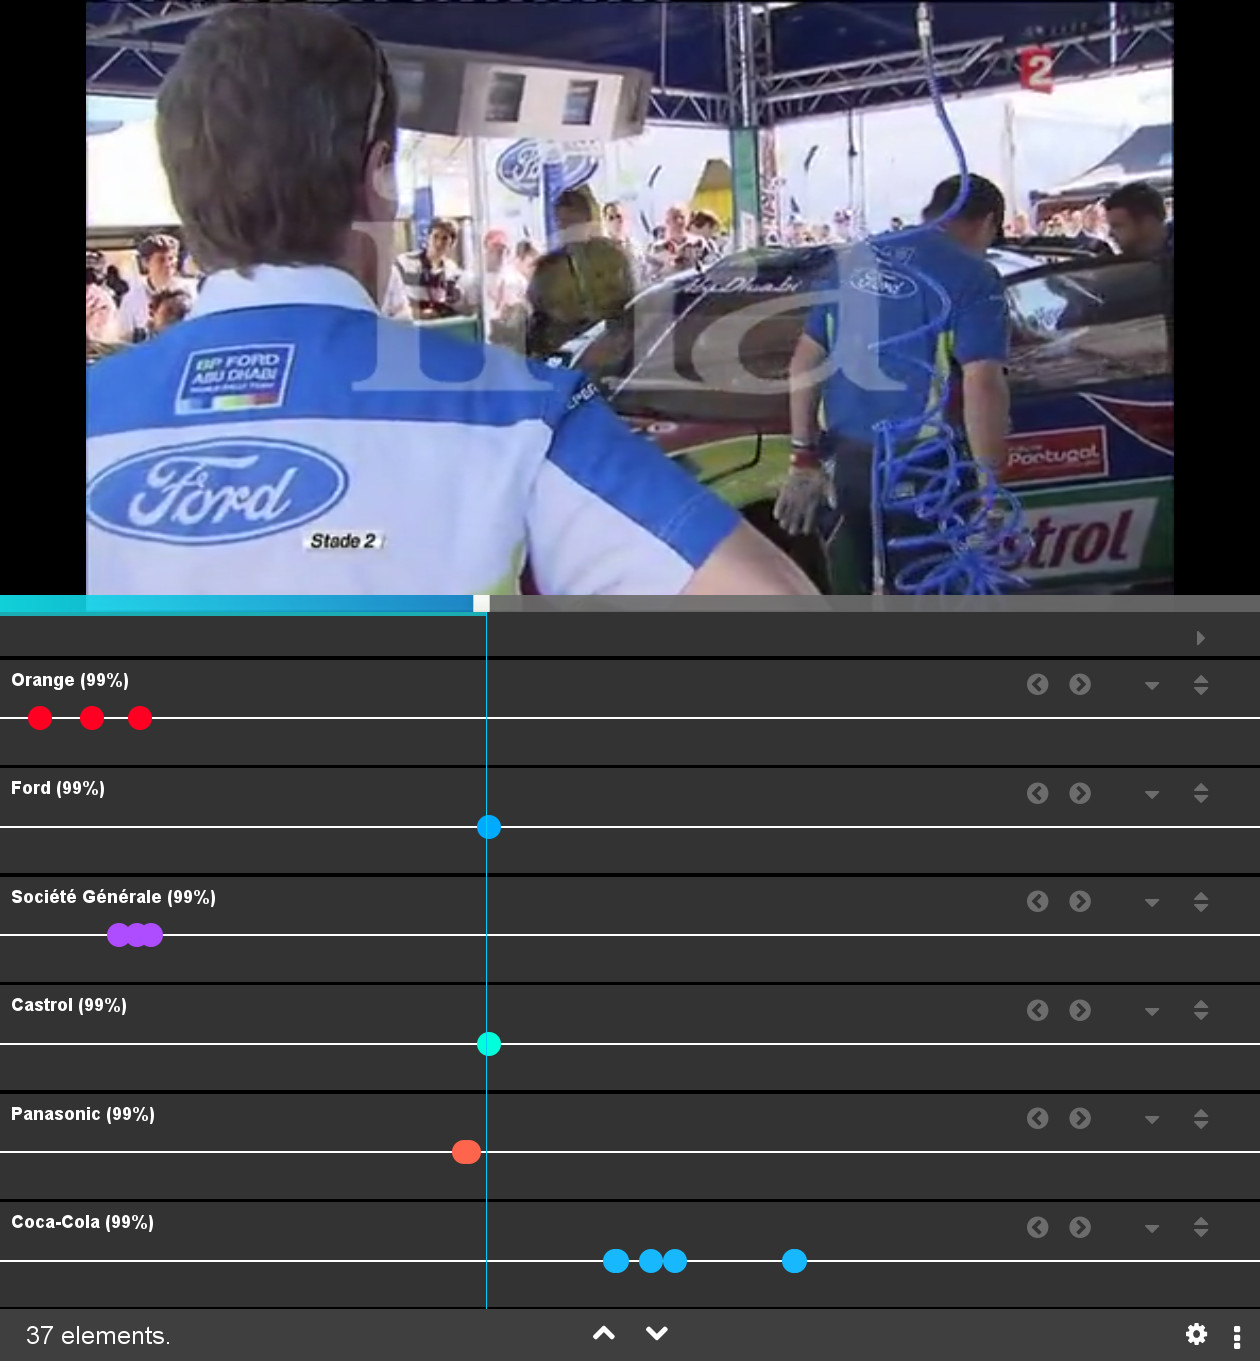
\includegraphics[width=10cm]{images/diginpix_resultat.jpg}
	\caption[Extraction des entités nommées d'un programme de France 2 avec DigInPix]{Extraction des entités nommées d'un programme de France 2 avec DigInPix [Source: \cite{institut_national_de_laudiovisuel_diginpix_nodate}]}
	\label{diginpix_result}
\end{figure}

Avec le projet du \index[ref]{led@Linked Enterprise Data (LED)!ldd@Lac de données (INA)}\index[ref]{modelisation@Modélisation!ldd@Lac de données (INA)}\ldd, la création de descriptions de contenus peut aller encore plus loin. En effet, le modèle de données unifié, comprenant l'ensemble des anciens référentiels de la \ac{ddcol}, permet de mettre en relation les données issues automatiquement d'un processus de traitement des vidéos par l'intelligence artificielle avec les concepts du \ldd. La segmentation automatique de vidéos\footnote{Le projet est SAAJ, Segmentation et Analyse Automatique des Journaux télévisés.} montre la diversité des utilisations possibles d'un référentiel quand celui-ci est uniforme et centralisé. Ce nouveau projet, au sein de celui du \ldd, débute en 2018 et conduit à la création de multiples outils, permettant tous une description automatique du contenu d'une vidéo --- les journaux télévisés et les chaînes d'information. Ainsi, la segmentation automatique par l'intelligence artificielle permet:
\begin{itemize}
	\item l'établissement d'une grille de programmation à partir des métadonnées fournies par les diffuseurs, les producteurs, \dots afin de déterminer les horaires prévus et habituels de chaque programme pour les chaînes d'information
	\item la classification automatique du programme ou des segments de programme selon une typologie précise --- plateau, présentateur, reportage, \dots
	\item la transcription des voix et de la parole, produisant ainsi un texte non formaté à partir duquel une description du contenu est effectuée avec des entités nommées qui en sont extraites et un alignement avec les entités de Wikidata
	\item l'océrisation des textes présents dans l'image, créant également un texte qui permet une description intellectuelle du contenu et un alignement des entités nommées avec Wikidata; cette océrisation concerne notamment les bandeaux des journaux télévisés dans lesquels le nom et la fonction de chaque personne sont indiqués
	\item la description automatique d'une image par un tagging d'entités nommées
	\item la reconnaissance de visages afin d'identifier le présentateur du journal télévisé, ou les protagonistes des vidéos
	\item la reconnaissance d'images et de logos, afin d'enrichir la description déjà précise de la vidéo ou du segment
\end{itemize} 

Chacun de ces outils fonctionne avec, ou en relation avec, un ou plusieurs référentiels: ils peuvent être internes, c'est à dire propres à l'\ac{ina}, ou bien externes comme Wikidata qui permet un enrichissement et une ouverture des métadonnées vers l'extérieur. Ces données générées automatiquement sont créées sous le modèle du \index[ref]{led@Linked Enterprise Data (LED)!ldd@Lac de données (INA)}\index[ref]{modelisation@Modélisation!ldd@Lac de données (INA)}\ldd et sont, par conséquent, en relation avec ses concepts. 

\subsection{\label{III-B-3-b}Faciliter et améliorer le catalogage des documents de l’\ac{ina} par l’extraction automatique de données}
\titreEntete{Faciliter et améliorer le catalogage des documents}

L'apport du projet SAAJ est une description fine et précise de l'ensemble d'une vidéo. Au-delà de la génération automatique de métadonnées dans le \index[ref]{led@Linked Enterprise Data (LED)!ldd@Lac de données (INA)}\index[ref]{modelisation@Modélisation!ldd@Lac de données (INA)}\ldd, il devient une aide pour le technicien de gestion des contenus multimédia de l'\ac{ina}. En effet, il n'a plus à créer les métadonnées associées au document, mais à superviser leur qualité et leur véracité: \og Le documentaliste « humain » est-il destiné à
passer du statut de producteur de données à celui de contrôleur de la qualité des fruits de l’automatisation ?\fg{}\footcite[p.134]{alquier_production_2017}. Cet aspect de contrôle qualité est un usage indirect des données générées automatiquement: il est positif pour la création précise, fine et complète de métadonnées sur un programme; mais il contraint à un changement de pratiques de catalogage, où l'humain n'a plus le rôle principal, qui est intellectuel, dans lequel il décrit le document et son contenu. \\

Cette amélioration et cette facilitation du travail de catalogage a lieu depuis des données nouvelles, générées par l'intelligence artificielle. Cependant, le contrôle de la qualité des métadonnées, et leur enrichissement, peuvent également passer par un traitement \textit{a posteriori}. En effet, l'apparition du Web sémantique et son adoption par un grand nombre d'institutions a poussé l'\ac{ina}, associé à d'autres institutions, à mener le projet Qualinca entre 2012 et 2015 afin \og d'améliorer la richesse, la cohérence et l’interopérabilité des métadonnées du système documentaire de l’Ina à travers la mise en œuvre d’une activité de recherche dans le domaine des techniques de liage de données\fg{}\footcite[p.129]{alquier_production_2017}. Qualinca repose sur de nombreux enjeux, comme la possibilité de partager des identifiants communs entre les différents métiers, l'amélioration des descriptions de contenus grâce aux données extérieures du \index[ref]{lod@Linked Open Data (LOD)}\ac{lod}, mais également d'effacer les ambiguïtés des termes des lexiques de l'\ac{ina}.\\

Se basant sur deux algorithmes, ProbFr et Agreg, Qualinca s'est surtout tourné vers les alignements de corpus de musique, et d'homonymes de personnes physiques et d'émissions. Dans cet alignement des homonymes avec le \index[ref]{lod@Linked Open Data (LOD)}\ac{lod}, la base \index[ref]{lod@Linked Open Data (LOD)!dbpedia@DBpédia}DBpedia --- Wikidata n'est né qu'en 2014 ---, les résultats sont peu exploitables et se heurtent, comme nous avons pu le constater lors de l'alignement des personnes physiques avec Wikidata, au langage naturel des fonctions que les algorithmes sont incapables de dépasser: sur 5000 \nP{Jacques}{Martin}, 667 différents ont été identifiés par les algorithmes\footcite[p.133]{alquier_production_2017}.\\

L'extraction automatique d'entités nommées a permis la création de nouvelles métadonnées, associées non pas au matériel ou aux données de diffusion mais au contenu intellectuel des vidéos, ainsi que l'apport d'une aide au \index[ref]{led@Linked Enterprise Data (LED)!ldd@Lac de données (INA)}\index[ref]{modelisation@Modélisation!ldd@Lac de données (INA)}catalogage par la qualité des entités fournies et leur précision.

\subsection{\label{III-B-3-c}Améliorer la valorisation des documents et offrir une meilleure expérience utilisateur}
\titreEntete{Améliorer la valorisation des documents}

La centralisation des données de l'\ac{ina} au sein du \index[ref]{led@Linked Enterprise Data (LED)!ldd@Lac de données (INA)}\index[ref]{modelisation@Modélisation!ldd@Lac de données (INA)}\ldd ouvre des possibilités pour la valorisation des documents auprès de tous les publics\footnote{Pour l'ensemble de l'offre disponible, voir la \reference{I-B}.}. D'abord, cette centralisation permet la création de multiples applications pour l'utilisateur, sans que cela ne modifie la structure des données\footnote{Voir \reference{annexe_lac} (\reference{lac_infra}).}; ainsi, la présence de l'\ac{ina} en est modifiée par l'apparition d'un \textit{hub} regroupant l'ensemble de l'offre numérique de l'Institut\footnote{\og L’autre grand défi posé à l’Institut, c’est celui de l’accessibilité de ses propositions. Les rassembler au sein d’un grand portail numérique, un hub qui offrira en quelques clics un accès renouvelé, simplifié et cohérent à l’ensemble des activités, contenus et services de l’Ina, est ainsi l’objectif qui mobilise aujourd’hui toute l’entreprise à l’horizon de 2019.\fg{} in \cite{vallet_ina_nodate}}.\\

Cette centralisation de l'offre est aussi présente pour les usages internes avec la création d'une nouvelle interface de consultation des métadonnées et des documents en eux-mêmes, Notilus, afin d'éviter la consultation croisée de multiples interfaces selon la provenance du document comme cela était le cas avant le \index[ref]{led@Linked Enterprise Data (LED)!ldd@Lac de données (INA)}\index[ref]{modelisation@Modélisation!ldd@Lac de données (INA)}\ldd. Par cette interface, le \ac{dl}, le \ac{da}, puis la \ac{dj} et l'ensemble des professionnels de l'\ac{ina}, ont accès aux mêmes données et aux mêmes documents, en un point unique, une interface de consultation qui reconstitue les instances du \ldd.\\

L'amélioration de l'expérience utilisateur est également une priorité dans une période où la modification des pratiques est radicale: ces pratiques sont quasiment toutes numériques et contraignent l'\ac{ina} à s'adapter. Si le site \url{https://www.ina.fr} est né dès 2009, le \index[ref]{led@Linked Enterprise Data (LED)!ldd@Lac de données (INA)}\index[ref]{modelisation@Modélisation!ldd@Lac de données (INA)}\ldd va pouvoir lui apporter d'importantes améliorations. En effet, la présence des référentiels y est limitée et restreint les possibilités de rebonds de la part de l'utilisateur\footnote{Voir \reference{inafr_result}.}. Ainsi, les liens des personnes au générique ne renvoient pas à une vedette personne de l'\ac{ina}, mais à des résultats de recherche sur le nom de cette personne. 
\begin{figure}[!h]
	\centering
	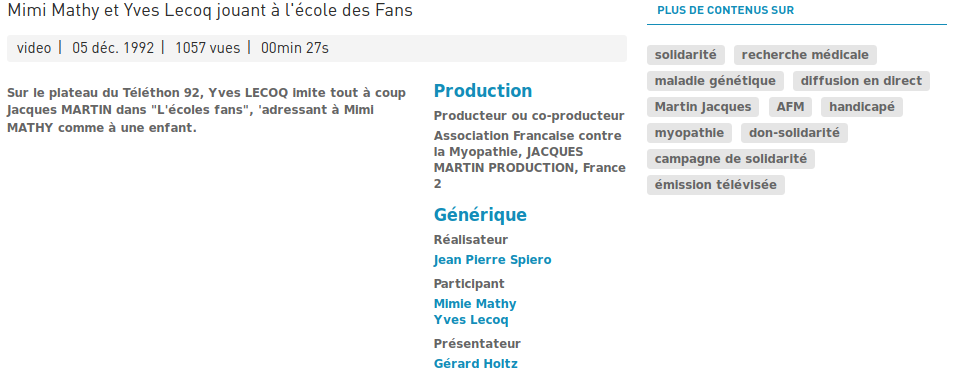
\includegraphics[width=13cm]{images/inafr_ecole_fans.png}
	\caption[Métadonnées associées à un document sur ina.fr]{Métadonnées associées à un document sur ina.fr [Source: \url{https://www.ina.fr/video/I11297765/mimi-mathy-et-yves-lecoq-jouant-a-l-ecole-des-fans-video.html}]}
	\label{inafr_result}
\end{figure}\\
Les possibilités offertes par le \ldd sont multiples et nous pouvons en imaginer certaines, basées sur le seul usage des concepts et de leurs relations, qui faciliteraient la recherche de l'utilisateur. Ainsi, comme pour la BnF, la création de vedettes de personnes est envisageable afin de regrouper en une même page les informations biographiques, ainsi que les documents liés (les instances) ou bien les thématiques principales (les concepts liés). Les termes d'indexation et de description des vidéos peuvent également être concernés par ce regroupement d'informations et de liens. Cependant, plus encore que ces regroupements de métadonnées, d'instances et de concepts relatifs à un concept, il est désormais possible, par les liens établis avec le \index[ref]{lod@Linked Open Data (LOD)}\ac{lod}, d'obtenir des informations manquantes et d'enrichir les données proposées à l'utilisateur: un lien peut être inséré, comme c'est le cas dans \index[ref]{lod@Linked Open Data (LOD)!viaf@VIAF}\index[ref]{autorites@Autorités!viaf@VIAF}\ac{viaf}, ou bien les champs peuvent être directement remplis sur la page HTML.\\

Ces possibilités ne sont envisageables que par la déconstruction de l'information dans le \ldd, permettant alors une grande modularité des données dans les usages qui en sont faits. Ces usages ne sont pas tous nés et le \index[ref]{led@Linked Enterprise Data (LED)!ldd@Lac de données (INA)}\index[ref]{modelisation@Modélisation!ldd@Lac de données (INA)}\ldd doit pouvoir permettre à l'\ac{ina} de les remplir sans avoir recours à un modification du modèle de données ou à la création d'une nouvelle de données. Ainsi, s'il est nécessaire de publier les données\footnote{Cet aspect semble difficile pour l'\ac{ina} en raison des données personnelles qui y sont conservées. Cependant, la loi de 2016 pour une République numérique (\cite{noauthor_loi_2016}) encourage à la publication des données de référence qui peuvent être réutilisées par d'autres services ou d'autres institutions.} sur le Web et plus particulièrement sur le Web de données, une représentation \index[ref]{echanges@Échanges!formats@Formats!rdf@RDF}\ac{rdf} est possible; avec la forte présence de l'\ac{ina} sur les réseaux sociaux, il peut être envisager de créer des publications automatiquement à partir de tags issus de concepts; \dots

%conclu
\bigskip
\bigskip
Le référentiel a atteint une place centrale dans le \ldd: l'ensemble des applications et des sites de l'Institut fonctionnent, ou vont fonctionner, depuis ce silo de métadonnées qui a été pensé selon la donnée et non plus selon les besoins. Ces derniers, évolutifs et dépendants de la période, ne peuvent pas tous être prédits, ce qui a conduit à la constitution d'un modèle de données souple et d'un processus intermédiaire de traitement de ces données, de manière à offrir à chaque application les données qui lui sont nécessaires.

	\chapter{\label{III-C}Centraliser les référentiels de l’INA dans le \ldd: l'exemple de l'alignement de deux référentiels de personnes physiques}
\titreEntete{Aligner deux référentiels de personnes physiques}

%intro
La \ac{ddcol} possède un unique référentiel de personnes physiques comme nous avons pu le constater plus tôt\footnote{Voir \reference{I-C-3} et \reference{II-C--3}.}. Le \ldd étant un \ac{led}, il tire son intérêt de la mise en commun de différentes bases de données et jeux de données. Ainsi, c'est l'ensemble des données et des métadonnées de l'\ac{ina} qui entrent dans ce \textit{Lac}: la base de données de la \ac{dj} fait alors l'objet de ce processus de migration vers le \ldd. Cependant, bien que la \ac{dj} représente un silo de données distinct de celui de la \ac{ddcol}, ils partagent tout de même certaines caractéristiques comme l'utilisation massive de personnes physiques, qui sont réunies dans un référentiel dans chaque service.\\

La migration des données de la \ac{ddcol} s'achève en fin d'année 2020 et laisse la place à celle de la \ac{dj}: afin d'éviter toute redondance de concepts dans le \ldd, il convient de rechercher pour une personne physique de la \ac{dj} son équivalent dans le \ldd --- par conséquent dans l'ancien référentiel des personnes physiques et morales de la \ac{ddcol} qui a été déconstruit sous forme de concepts\footnote{Voir \reference{III-B}.}. L'exécution de cet alignement montre à lui seul les problématiques liées au langage naturel, ainsi que la nécessaire présence humaine qui doit superviser les résultats issus d'une automatisation de tâches.

\section{\label{III-C-1}Des jeux de données différents en de multiples points}
\titreEntete{Des jeux de données différents}

%intro
L'alignement des personnes physiques de la \ac{ddcol} avec Wikidata avait déjà démontré l'importance de la donnée structurée afin de créer des points de contacts entre les deux jeux de données et de procéder à leur alignement. Les problématiques liées à la graphie et aux différences de structure ont aussi compliqué cet alignement. Dans le cadre de la mise en relation entre le référentiel des personnes physiques de la \ac{dj} avec celui de la \ac{ddcol}, ces points de contact sont réduits au minimum et peuvent interroger quant à la possibilité de réaliser des alignements sûrs, ou les plus sûrs possibles.

\subsection{\label{III-C-1-a}Enjeux}
\titreEntete{Enjeux}

Le \ldd n'étant pas conçu à partir des\index[ref]{led@Linked Enterprise Data (LED)!ldd@Lac de données (INA)}\index[ref]{modelisation@Modélisation!ldd@Lac de données (INA)} besoins métier mais des données, le référentiel des personnes physiques de la \ac{dj}, se présentant sous la forme d'une table \textit{PERSONNE} de la base de données, ne peut pas être conservé dans sa structure actuelle. En effet, il est uniquement adapté aux besoins de la \ac{dj} et ne correspond pas aux usages que pourrait en faire la \ac{ddcol} ou l'utilisateur final des applications de l'\ac{ina}. Afin d'intégrer ce référentiel dans le \textit{Lac}, il est nécessaire de l'aligner avec les concepts existants, issus du référentiel des personnes physiques de la \ac{ddcol}. Ainsi, un double enrichissement a lieu, celui des concepts par les données de la \ac{dj}, et celui de la \ac{dj} par les données des concepts. Cependant, cet enrichissement devient invisible dans le \ldd puisqu'il n'y a plus de notion de référentiel, et que les distinctions entre \ac{dj} et \ac{ddcol} sont volontairement effacées au profit d'une structure de données plus souple.\\

Cet alignement a pour finalité l'ajout d'un lien \textit{provenance--\ac{dj}} à un concept quand le matricule de la \ac{dj} et le concept sont identiques, ou bien la détection des nombreuses personnes de la \ac{dj} qui ne sont pas des concepts. En effet, la \ac{dj} ayant pour fonction de repérer les ayants-droits et ouvrants-droits de personnes liées à un extrait audiovisuel, ceux-ci ne sont, par conséquent, pas spécifiquement dans la description des documents audiovisuels réalisée par la \ac{ddcol} car ils n'interviennent à aucun moment dans ces documents. Ainsi, nombreuses sont les personnes de la \ac{dj} qui n'ont pas d'équivalent dans la \ac{ddcol} et qu'il est nécessaire de repérer afin de leur créer \textit{in fine} un concept dans le \index[ref]{led@Linked Enterprise Data (LED)!ldd@Lac de données (INA)}\index[ref]{modelisation@Modélisation!ldd@Lac de données (INA)}\ldd.\\

Cette différence entre les jeux de données montre une nouvelle fois comment se sont formées les bases de données --- selon les usages et les besoins --- qui sont à migrer dans le \index[ref]{led@Linked Enterprise Data (LED)!ldd@Lac de données (INA)}\index[ref]{modelisation@Modélisation!ldd@Lac de données (INA)}\ldd: à cause de cette différence, il devient difficile d'estimer l'efficacité et le rendement du processus d'alignement qui va être réalisé. En effet, connaître la raison de l'absence d'alignement de certains matricules des personnes de la \ac{dj} sera uniquement possible par une action humaine. Face à ces enjeux et aux problématiques soulevées par le seul historique des bases de données, l'alignement des deux référentiels comporte plusieurs difficultés supplémentaires déjà évoquées dans les chapitres précédents.

\subsection{\label{III-C-1-b}Points de contact}
\titreEntete{Points de contact}

Trouver des points de contact entre deux jeux de données, plus encore entre deux référentiels, est essentiel lors d'un alignement: plus ces points de contact sont nombreux, plus les comparaisons sont nombreuses et les alignements sûrs. Cependant, les référentiels de la \ac{ddcol} et la \ac{dj} n'en partagent que peu --- sept. De plus, ces points de contact nécessitent la présence de l'information de chaque côté, ce qui est peu la cas entre la \ac{dj} et la \ac{ddcol}.\\

Dans le \index[ref]{led@Linked Enterprise Data (LED)!ldd@Lac de données (INA)}\index[ref]{modelisation@Modélisation!ldd@Lac de données (INA)}\ldd, les concepts disposent notamment d'attributs indiquant le nom, le sexe, les dates de naissance et de décès, ainsi que la note qualité. Cette note qualité n'étant pas scindée dans le \ldd, il est nécessaire, dans cet alignement, d'en extraire la fonction, ou les fonctions, de la personne, en supprimant la mention des pays d'exercice.\\

Si la \ac{dj} dispose de nombreuses données personnelles pour mener à bien ses missions, les données permettant un alignement documentaire sont plus restreintes: hormis le nom et le sexe, seule une date de décès est disponible, ainsi qu'une contribution. En effet, seule la date de décès intéresse le service juridique pour ses applications dans le droit et le reversement des droits aux ayants-droits ou ouvrants-droits: conserver une date de naissance n'a par conséquent aucun usage dans la \ac{dj}.

\noindent Le référentiel des personnes de la \ac{dj} présente une petite normalisation avec les contributions: celles-ci ne sont pas du texte libre, mais du texte contrôlé et choisi parmi une liste d'une vingtaine d'entrées. Ce contrôle du vocabulaire permet, dans l'alignement, des rendements meilleurs après, nous le verrons, un traitement préalable des données des notes qualité de la \ac{ddcol}.\\

Cependant, les points de contact identifiés pour la \ac{dj} et la \ac{ddcol} sont peu nombreux, ce qui complique la détection des homonymes et diminue la fiabilité des alignements futurs.

\subsection{\label{III-C-1-c}Divergences}
\titreEntete{Divergences}

En plus de ces difficultés sur la quantité des points de contact, les deux référentiels diffèrent par leurs structures et leurs graphies. Tout d'abord, les niveaux de description des mêmes attributs sont différents. En effet, alors que le nom du concept du \index[ref]{led@Linked Enterprise Data (LED)!ldd@Lac de données (INA)}\index[ref]{modelisation@Modélisation!ldd@Lac de données (INA)}\ldd est composé de la forme \og \textit{Nom, Prénom}\fg{}, l'état-civil stocké à la \ac{dj} est divisé en deux attributs: un nom et un prénom. Ainsi, avant d'effectuer l'alignement, il est nécessaire de scinder le nom du concept afin de récupérer le nom et le prénom séparément.

\noindent Le jeu de données de la \ac{dj} offre également deux autres attributs, les pseudos de nom et de prénom de chaque personne. Afin d'utiliser ces deux attributs supplémentaires, il est nécessaire de leur trouver un point de contact dans les concepts issus de la \ac{ddcol}: ainsi, il a été considéré qu'un nom de concept ne possédant pas de virgule est un pseudo. Par conséquent, ce pseudo, issu des concepts, peut être comparé avec le pseudo du nom de la \ac{dj}\footnote{Dans les données de la \ac{dj}, c'est le pseudo-nom qui comporte le pseudonyme courant d'une personne; l'attribut pseudo prénom n'est utilisé que pour indiquer une variante du prénom de cette personne.}.\\

En plus de ces différences de niveaux de description, les graphies ne sont pas les mêmes. D'abord, les données de la \ac{dj} sont en majuscules, alors que celles de la \ac{ddcol} sont en minuscules. Si cette difficulté n'est pas majeure, elle nécessite tout de même un traitement dans l'ETL avant de pouvoir procéder à un alignement. De même, afin d'éviter toute variation dans des chaînes de caractères renvoyant à une même personne mais aux graphies différentes, les accents et la ponctuation sont retirés. Les dates, commee lors des alignements décrits dans les chapitres précédents, sont réduites à la seule année.

\noindent La difficulté majeure, posée dans l'alignement de deux référentiels de personnes, est la graphie et l'utilisation des particules des noms. En effet, l'utilisation des particules n'est pas normalisée dans l'Institut, ce qui conduit à la présence de \nP{Louis de }{Funès} dans la \ac{ddcol}, alors que la \ac{dj} conserve la forme \nP{Louis}{de Funès}. Les pratiques d'écriture des noms à particules étant constantes à la \ac{ddcol}, il est possible de transférer cette particule\footnote{Cette particule n'est pas exclusivement \textit{de}, elle peut être de l'une des formes suivantes: \textit{de, des, du, de la}} dans le nom afin d'obtenir  \nP{Louis}{de Funès} dans chaque jeu de données.\\

Enfin, afin de donner aux alignements une plus grande fiabilité, il est essentiel de prendre en compte le texte des notes qualité pour le comparer avec les contributions de la \ac{dj}. Les notes qualité de la \ac{ddcol} comportant plus de vingt mille fonctions différentes, il n'est pas possible de les faire correspondre chacune avec l'une des contributions de la \ac{dj}. Pour cela, seules les contributions et les fonctions des notes qualité les plus courantes ont fait l'objet d'un alignement manuel pour faciliter l'alignement automatique qui va suivre; cinq de ces contributions ont ainsi été pu être traitées:
\begin{itemize}
	\item le terme \textit{Journalisme} de la \ac{dj} est remplacé par \og journaliste\fg{};
	\item \textit{Artiste interprètre} est remplacé par \og chanteu\fg{}\footnote{Les terminaisons sont enlevées dans ces termes de remplacement afin de prendre en compte les variantes de graphie liées au pluriel et au féminin que l'on peut trouver dans les fonctions de la \ac{ddcol}.}
	\item \og realisat\fg remplace \textit{Réalisation}
	\item \og composit\fg remplace \textit{Composition musicale}
	\item enfin, \textit{Réalisation associée} est remplacé par \og realisat\fg{}
\end{itemize}
\medskip
Les chanteurs, les compositeurs, les réalisateurs et les journalistes étant les fonctions les plus courantes dans les deux jeux de données, elles ont été repérées puis traitées. Cependant, une majorité de fonctions ne pourra pas être alignée avec les contributions de la \ac{dj}, et par conséquent limitera la confiance accordée aux alignements.


%conlu
\bigskip
\bigskip
La centralisation de référentiels et de données est nécessaire pour les systèmes documentaires, mais la reprise de ces référentiels et de ces données peut être compliquée par les structures et les normes divergentes selon les jeux de données. Cette absence d'uniformisation annonce déjà des résultats faibles et limités dans la confiance qui peut être accordée. Dans le cas de l'alignement des référentiels de personnes physiques de la \ac{dj} et de la \ac{ddcol} à l'\ac{ina}, les points de contacts sont peu nombreux et peu spécifiques\footnote{Voir \reference{table_contact_dj_ddcol}.}.

\begin{table}[!h]
	\centering
	\begin{tabular}{|c|c|}
		\hline
		\textbf{\ac{dj}} & \textbf{\ac{ddcol}}\\ \hline
		Nom&Nom\\ \hline
		Prénom&Prénom\\ \hline
		Pseudo nom&Pseudo\\ \hline
		Pseudo prénom&\\ \hline
		Sexe&Sexe\\ \hline
		Date de naissance&Date de naissance\\ \hline
		Contribution&Fonction\\ \hline
	\end{tabular}
	\caption[Points de contact entre les référentiels de la \ac{dj} et de la \ac{ddcol}]{Points de contact entre les référentiels de la \ac{dj} et de la \ac{ddcol}}
	\label{table_contact_dj_ddcol}
\end{table}

\section{\label{III-C-2}Établir une méthodologie particulière d'alignement}
\titreEntete{Une méthodologie particulière}

%intro
En raison des difficultés identifiées dans la \reference{III-C-1}, un alignement simple, n'apportant aucune indication de fiabilité, n'est pas possible. De même, les alignements réalisés dans les chapitres précédents utilisent chacun les jeux de données initiaux jusqu'à la fin du traitement, sans en retirer au fur et à mesure les concepts qui viennent d'être alignés. L'alignement des référentiels de la \ac{ddcol} et de la \ac{dj} se distingue des précédents par la nécessité d'une méthodologie particulière, basée sur un indice de confiance attribué à chaque alignement, et sur une succession d'étapes, représentant les niveaux de confiance apportés au type de jointure utilisé.

\subsection{\label{III-C-2-a}Créer un indice de confiance pour chaque alignement}
\titreEntete{Créer un indice de confiance}

Les points de contact entre les jeux de données n'ont pas tous la même valeur dans un alignement. En effet, l'état civil d'une personne, bien qu'essentiel dans un alignement, peut conduire à aligner deux homonymes: c'est pourquoi les points de contact comme les noms, les prénoms ou les pseudos peuvent être considérés comme ayant une faible valeur dans le processus d'alignement. De plus, leur octroyer une valeur forte conduirait à surévaluer les alignements réalisés sur la simple comparaison des noms et prénoms sans autre point de comparaison par rapport aux alignements qui n'auront pas été possibles.\\

En revanche, la valeur des points de comparaison significatifs est considérée comme forte: il s'agit de la date de décès ou de la contribution. En effet, la probabilité que les états civils et les dates de décès de deux homonymes soient identiques est très faible, ce qui peut permettre de donner à cet alignement une valeur plus forte. De même, la correspondance entre une contribution et une fonction est considérée comme très fiable quand les états civils ont déjà été rapprochés: pour cette raison, le point de comparaison sur la contribution est celui qui possède l'indice de confiance le plus élevé, puisqu'il est le point le plus spécifique, et le plus difficile à faire correspondre.\\

Enfin, la comparaison du sexe permet également d'augmenter la fiabilité d'un alignement. Dans la majorité des alignements qui sont réalisés, la comparaison peut sembler évidente à l'humain, mais dans certains cas, comme pour les prénoms \textit{Dominique}, elle est nécessaire et permet la conservation ou non de l'alignement.\\

L'indice de confiance permet une priorisation des points de comparaison, une hiérarchisation de ces derniers. Il se forme à partir de la somme des scores de chaque point de comparaison. Ainsi, dans le cas de l'alignement des référentiels de personnes de la \ac{dj} et de la \ac{ddcol}, l'indice de confiance varie entre 0 --- quand l'alignement n'a pas pu être réalisé --- et 9 --- quand tous les points de comparaison ont été réalisés avec succès --- selon les scores de la \reference{table_scores}.
\begin{table}[!h]
	\centering
	\begin{tabular}{|c|c|}
		\hline
		\textbf{Point de comparaison}&\textbf{Score}\\ \hline
		Nom&1\\ \hline
		Prénom&1\\ \hline
		Pseudo nom&1\\ \hline
		Pseudo prénom&1\\ \hline
		Sexe&1\\ \hline
		Date de décès&2\\ \hline
		Contribution&2\\ \hline
	\end{tabular}
	\caption{Scores attribués à chaque point de comparaison}
	\label{table_scores}
\end{table}

\subsection{\label{III-C-2-b}Des étapes exclusives}
\titreEntete{Des étapes exclusives}

L'attribution d'un indice de confiance ne permet de résoudre que la problématique de l'évaluation finale des alignements. Il subsiste néanmoins une seconde problématique, celle de la présence dans les alignements réalisés de doublons, c'est à dire de personnes de la \ac{dj} alignés avec plusieurs concepts. Une solution pourrait être de supprimer les alignements présents dans ce cas. Or, ce cas survient fréquemment: supprimer les alignements concernés réduirait la quantité de résultats finaux.\\

Ainsi, après une première priorisation des points de comparaison, il est nécessaire d'effectuer ensuite une priorisation des combinaisons de ces points de comparaison. Quatre étapes principales ont été identifiées et constituent cette priorisation.

\noindent D'abord, les alignements réalisés avec le nom, le prénom, les pseudos et la correspondance des fonctions sont considérés comme ceux étant les plus sûrs pour effectuer les rapprochements entre les concepts de la \ac{ddcol} et les matricules de la \ac{dj}. Ces alignements, comme ceux des étapes suivantes, sont des jointures\footnote{Afin de ne récupérer que les alignements qui ont été réalisés, ces jointures sont de type \textit{inner join}.} entre les deux jeux de données réalisées dans l'ETL Talend avec le composant associé, un tMap (\reference{tmap_jointures}).
\begin{figure}[!h]
	\centering
	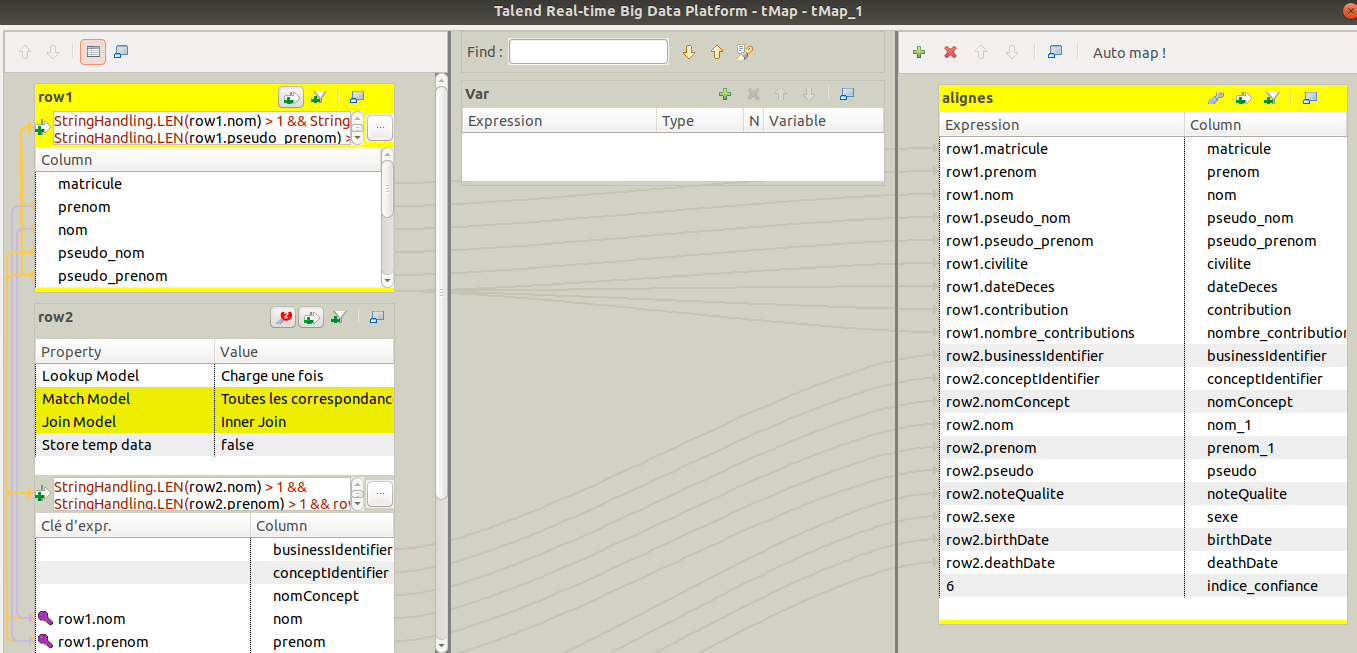
\includegraphics[width=16cm]{images/tmpa_jointure1_dj.png}
	\caption{L'alignement des personnes de la \ac{dj} et de la \ac{ddcol} pour une jointure dans un tMap de Talend.}
	\label{tmap_jointures}
\end{figure}

\noindent Ensuite, les alignements effectués avec le nom, le prénom et les pseudos, sans avoir pu faire correspondre les fonctions, sont la seconde étape.

\noindent La troisième étape, comme la quatrième, tente de rapprocher deux personnes en prenant en compte les différences de graphie qui peuvent exister. Ainsi, les alignements sont réalisés sur les pseudos, et sur le prénom de la \ac{dj} commençant par le prénom de la \ac{ddcol}\footnote{Une exception a été créé dans cette étape pour les prénoms \textit{Jean} et \textit{Anne}.}. Cette étape permet l'alignement d'une même personne ayant à la \ac{ddcol} le prénom \textit{Louis} et à la \ac{dj} le prénom \textit{Louis Marie}.

\noindent Enfin, l'ensemble des combinaisons possibles étant couvert, il est nécessaire d'effectuer une dernière étape pour effectuer non pas des alignements fiables --- ce qui est le but des trois premières étapes --- mais des alignements permettant d'apporter une aide à un opérateur humain en proposant plusieurs concepts qu'il est possible d'aligner avec un matricule. Ce rapprochement particulier, réalisé sur les seuls nom et prénom, autorise par conséquent la présence de plusieurs concepts alignés avec un même matricule, notamment dans le cas d'homonymes.\\

Distinguer ces quatre étapes permet, à l'issue de chacune d'elles, de récupérer ce qui n'a pas été aligné, tant du côté de la \ac{dj} et de la \ac{ddcol}, afin d'effectuer l'étape suivante avec uniquement ces données non alignées (\reference{orchestration}). Cette récupération évite de créer des alignements doubles avec des concepts différents entre les étapes. C'est également à l'issue de cette récupération que les résultats des jointures précédentes sont comparés afin de supprimer les matricules alignés plusieurs fois, et d'attribuer les scores pour le sexe et la date.\\
\begin{figure}[!h]
	\centering
	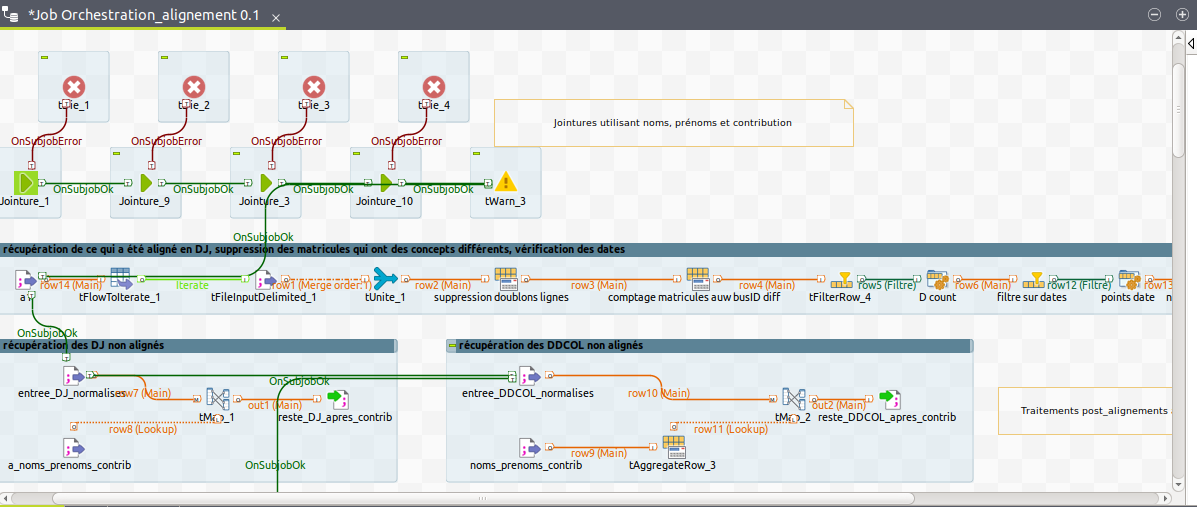
\includegraphics[width=16cm]{images/orchestration_partie1_dj.png}
	\caption{L'orchestration de la première étape dans l'ETL Talend.}
	\label{orchestration}
\end{figure}

Cependant, la limite de la récupération des matricules des personnes non alignées de la \ac{dj} et de la \ac{ddcol} est dans la priorisation qui a été faite des étapes. En effet, elle se base uniquement sur des critères définis en amont par un humain selon l'observation des cas généraux d'alignements: bien que ce soit une méthode apportant de la fiabilité aux alignements, cette fiabilité n'est pas nécessairement celle qui est la plus optimale. De même, cette récupération pourrait avoir lieu après chaque alignement de matricule: cela ajouterait néanmoins une nouvelle priorisation, basée sur l'ordre de passage, qui est plus arbitraire encore, puisque cet ordre de passage des matricules de la \ac{dj} dans le processus d'alignement n'est régi par aucun ordre significatif\footnote{Une base de données relationnelle n'étant pas ordonnée.}.

%conlu
\bigskip
\bigskip
Face aux nombreuses difficultés, l'indice de confiance et la priorisation des étapes permettent de réduire les mauvais alignements, et d'apporter une précision sur la fiabilité d'un alignement. Cependant, l'automatisation de ce processus présente des limites comme la définition de règles dirigeant le processus d'alignement. L'alignement des soixante-dix mille matricules de la \ac{dj} et des plus de trois cent mille concepts de la \ac{ddcol} ne peut pas être réalisé sur la base de quelques règles puis être considéré comme fiable.
\section{\label{III-C-3}Des résultats à la hauteur des données initiales}
\titreEntete{Des résultats à la hauteur des données initiales}

%intro
Les résultats de l'automatisation d'un processus de traitement de données dépend entièrement de la qualité des données initiales. Les difficultés propres aux différences de structures entre les jeux de données ou aux différences de graphie, additionnées à celles posées par la volonté d'avoir des alignements fiables et sans doublons, sont autant de facteurs qui réduisent l'efficacité de l'alignement automatique de deux référentiels.\\

Dans le cas de l'alignement des référentiels de personnes de la \ac{dj} et de la \ac{ddcol}, les résultats reflètent les difficultés rencontrées, tant dans les quantités de résultats que dans les indices de confiance attribués. Cette hétérogénéité des résultats conduit à la nécessité d'une supervision humaine des alignements réalisés et non réalisés.

\subsection{\label{III-C-3-a}Des résultats hétérogènes reflétant les multiples difficultés}
\titreEntete{Des résultats hétérogènes}

Environ soixante pour cent des matricules de personnes de la \ac{dj} ont trouvé leur équivalent dans la \ac{ddcol}. Ce résultat, bien que faible, reflète les difficultés rencontrées, ainsi que la spécificité des usages de chaque référentiel. En effet, la \ac{dj} utilise les personnes pour leur verser des droits, ce qui signifie alors que ces personnes ne sont pas spécialement des acteurs des documents conservés à la \ac{ddcol} pour lesquels le référentiel des personnes physiques a été créé. Il est par conséquent normal de ne pas pouvoir aligner tous les matricules de la \ac{dj} avec la \ac{ddcol}, cette dernière n'ayant pas besoin de conserver les ayants-droits de chaque personne du référentiel.

\begin{figure}[!h]
	\centering
	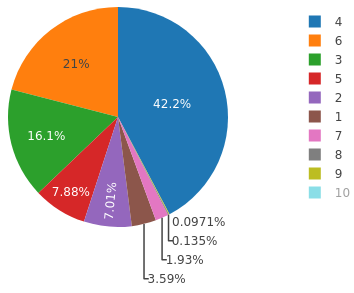
\includegraphics[width=8cm]{images/indices.png}
	\caption{Répartition des indices de confiance après les alignements entre les rééfrentiels de personnes de la \ac{dj} et de la \ac{ddcol}}
	\label{indices}
\end{figure}

La répartition des indices de confiance (\reference{indices}) reflète quant à elle à la fois la qualité des données initiales, ainsi que le processus d'alignement en lui-même. En effet, les différences de niveaux de précision dans les jeux de données initiaux conduisent à l'impossibilité d'utiliser certains points de comparaison, ce qui réduit l'indice de confiance: ces différences peuvent être une absence de données d'un côté de l'alignement, ou bien une divergence de graphie ou de structure qui n'a pas pu être corrigée lors du traitement préalable des données. Ainsi, l'indice \textit{4} est celui le plus présent en raison du faible nombre de points de comparaison qui le permettent: le nom, le prénom ainsi que la date ou une fonction suffisent à attribuer cet indice.\\

De plus, l'enchaînement des étapes entraîne également une diminution des indices de confiance: les étapes considérées comme prioritaires sont aussi celles qui utilisent les points de comparaison à la plus forte valeur. Ainsi, les indices de confiance attribués dans les alignements sont globalement inférieurs à cinq, et peu peuvent être considérés comme fiables quand l'indice est supérieur à cinq ou six.

\subsection{\label{III-C-3-b}Une supervision humaine nécessaire}
\titreEntete{Une supervision humaine nécessaire}

L'incertitude entourant la majorité des alignements conduit, comme cela est le cas pour le catalogage après la génération automatique de données, à utiliser une supervision humain. En effet, seule l'expertise et la réflexion d'un agent humain peut, ou non, confirmer les alignements produits. Seulement, cet agent humain va se heurter également à certaines problématiques posées dans l'automatisation: l'absence d'informations dans un matricule de la \ac{dj} ou dans un concept du \ldd ne permettra pas d'affirmer si les deux personnes alignées automatiquement sont réellement identiques et peuvent être associées.\\

Outre ce rejet ou cette acceptation des alignements réalisés automatiquement, la supervision humaine doit pouvoir modifier ce qui lui est proposé, ou bien pouvoir créer de nouveaux alignements. En effet, les jointures effectuées dans Talend\footnote{Elles sont au nombre de onze.} ne prennent pas en compte toutes les possibilités des deux jeux de données\footnote{Il existe quarante-deux (sept attributs sont disponibles dans la \ac{dj}, et six dans la \ac{ddcol}) jointures de stricte égalité possibles.} pour des raisons de fiabilité de ces possibilités dans le processus d'alignement. L'agent humain est seul capable de rechercher dans les données de la \ac{ddcol} un concept selon des critères que l'intelligence humaine offre: ils peuvent être l'inversion de deux lettres suite à une coquille dans la graphie, la francisation ou la traduction d'un terme étranger, l'inversion de deux prénoms, la connaissance d'un autre pseudonyme de la personne qui n'est pas spécifié dans les données de la \ac{dj}, \dots

%conlu
\bigskip
\bigskip
L'action humaine est toujours nécessaire, même avec un processus automatique d'alignement entre des données. Cette action est essentielle pour obtenir des données cohérentes et fiables dans un nouveau modèle de données. En effet, ces données étaient initialement cohérentes et sûres dans leurs bases de données respectives: elles doivent retrouver cette cohérence et cette fiabilité, même après un traitement automatique. Pour cela, la supervision humaine est nécessaire pour s'en assurer et proposer le cas échéant des solutions. 

%conclu
\bigskip
\bigskip
Dans le projet de centralisation des données de l'\ac{ina}, la centralisation des référentiels est indispensable, ces derniers étant devenus les pivots du système d'information. La conservation d'un référentiel utilisé par un seul jeu de données, celui de la \ac{dj}, ne correspond pas aux principes du \ac{led} et du \ldd. Ainsi, sa migration dans ce \textit{Lac} a nécessité un traitement important pour aboutir à l'alignement de ses matricules avec les concepts du \ldd. Face aux résultats de cet alignement, l'indice de confiance attribué permet une meilleure visibilité du travail effectué automatiquement, et permet aux superviseurs, qui sont nécessaires, d'approuver ou de refuser chaque alignement, afin d'éviter l'introduction d'erreurs dans le \ldd.
	
	\newpage
	
	%conclu
	%schéma global
	%le rféérentiel est passé au centre de tous les systèmes

	\chaptertoc{Conclusion}
\titreEntete{Conclusion}

%historique de struct ref: arbre au laby et modele reseau

%changement des usages et des besoins...

%... qui produit changement place ref
	
	\appendix
	\part*{Annexes}	
	\addcontentsline{toc}{part}{Annexes}
	\setcounter{chapter}{0}

\chapter{\label{annexe_index_schoepflin}Les index de la Renaissance, termes contrôlés et classification alphabétique (les index de l'\textit{Alsatia Illustrata} de \nP{Jean-Daniel}{Schoepflin})}
\titreEntete{Annexe \thechapter}

\begin{figure}[!h]
	\centering
	\begin{minipage}[c]{.46\linewidth}
		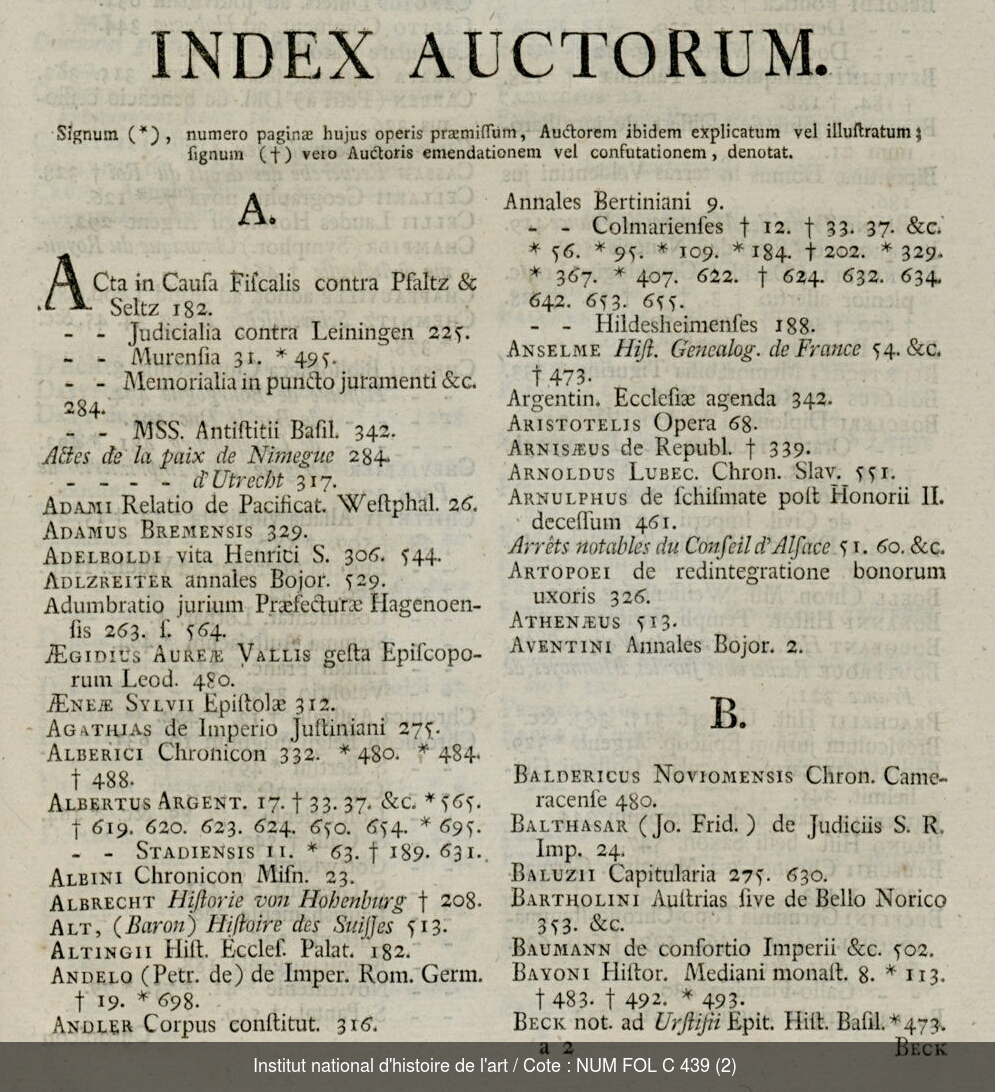
\includegraphics[width=6cm]{images/index_auctorum_alsatia.jpg}
		\caption{Index auctorum}
	\end{minipage} \hfill
	\begin{minipage}[c]{.46\linewidth}
		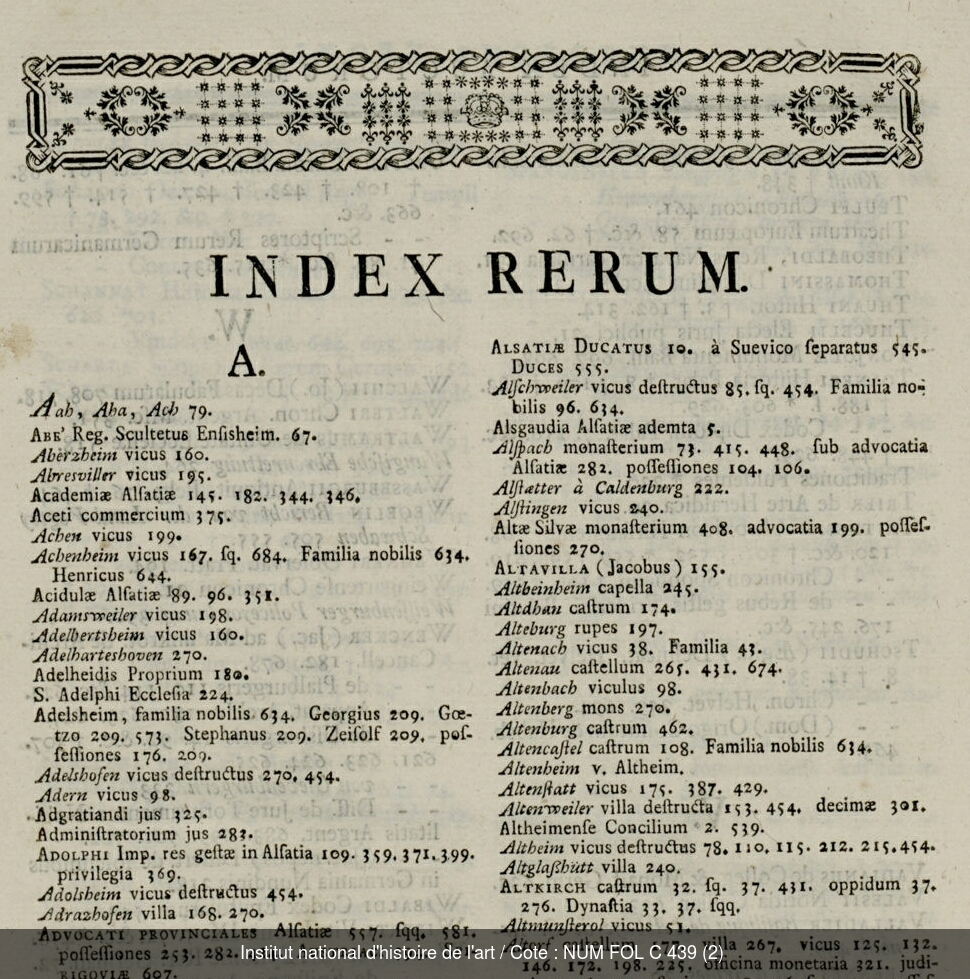
\includegraphics[width=6cm]{images/index_rerum_alsatia.jpg}
		\caption{Index rerum}
	\end{minipage} 
	\medskip
	Extraits des deux index de l'œuvre de \nP{Jean-Daniel}{Schoepflin} [Source: \url{http://bibliotheque-numerique.inha.fr/idurl/1/12532}, p.804 et 813]
\end{figure}

\chapter{\label{annexe_types_interop}Les différents types d'interopérabilité}
\titreEntete{Annexe \thechapter}

\begin{figure}[!h]
	\centering
	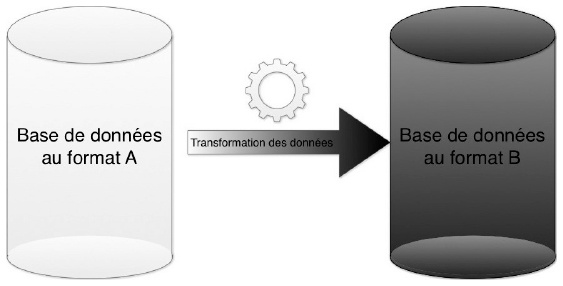
\includegraphics[width=12cm]{images/interop_conversion_copie.jpeg}
	\medskip
	\caption[L'interopérabilité par conversion et copie]{L'interopérabilité par conversion et copie [Source: \cite{bermes_2_2013}]}
\end{figure}

\begin{figure}[!h]
	\centering
	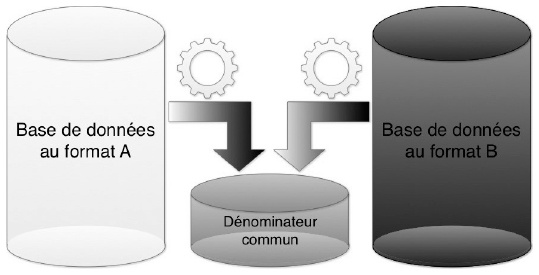
\includegraphics[width=12cm]{images/interop_denom_commun.jpeg}
	\medskip
	\caption[L'interopérabilité par le plus petit dénominateur commun]{L'interopérabilité par le plus petit dénominateur commun [Source: \cite{bermes_2_2013}]}
\end{figure}
	
	\backmatter
	
	
%bibliographie ici dans les normes de l'école
%\printbibliography[title= Bibliographie sélective, prenote=intro]%postnote est aussi possible
%\printbibliography[heading=subbibliography, keyword={semantique}, title={Sémantique}]%biblio sélective pour un mot clé donné

\printindex[referentiels]
\printindex[ina]

	\listoffigures
	
	\listoftables

	\tableofcontents
	
\end{document}